%%%%%%%%%%%%%%%%%%%%%%%%%%%%%%%%%%%%%%%%%
% The Legrand Orange Book
% LaTeX Template
% Version 2.4 (26/09/2018)
%
% This template was downloaded from:
% http://www.LaTeXTemplates.com
%
% Original author:
% Mathias Legrand (legrand.mathias@gmail.com) with modifications by:
% Vel (vel@latextemplates.com)
%
% License:
% CC BY-NC-SA 3.0 (http://creativecommons.org/licenses/by-nc-sa/3.0/)
%
% Compiling this template:
% This template uses biber for its bibliography and makeindex for its index.
% When you first open the template, compile it from the command line with the 
% commands below to make sure your LaTeX distribution is configured correctly:
%
% 1) pdflatex main
% 2) makeindex main.idx -s StyleInd.ist
% 3) biber main
% 4) pdflatex main x 2
%
% After this, when you wish to update the bibliography/index use the appropriate
% command above and make sure to compile with pdflatex several times 
% afterwards to propagate your changes to the document.
%
% This template also uses a number of packages which may need to be
% updated to the newest versions for the template to compile. It is strongly
% recommended you update your LaTeX distribution if you have any
% compilation errors.
%
% Important note:
% Chapter heading images should have a 2:1 width:height ratio,
% e.g. 920px width and 460px height.
%
%%%%%%%%%%%%%%%%%%%%%%%%%%%%%%%%%%%%%%%%%

%----------------------------------------------------------------------------------------
%	PACKAGES AND OTHER DOCUMENT CONFIGURATIONS
%----------------------------------------------------------------------------------------


\documentclass[11pt,fleqn]{book} % Default font size and left-justified equations
%%%%%%%%%%%%%%%%%%%%%%%%%%%%%%%%%%%%%%%%%
% The Legrand Orange Book
% Structural Definitions File
% Version 2.1 (26/09/2018)
%
% Original author:
% Mathias Legrand (legrand.mathias@gmail.com) with modifications by:
% Vel (vel@latextemplates.com)
% 
% This file was downloaded from:
% http://www.LaTeXTemplates.com
%
% License:
% CC BY-NC-SA 3.0 (http://creativecommons.org/licenses/by-nc-sa/3.0/)
%
%%%%%%%%%%%%%%%%%%%%%%%%%%%%%%%%%%%%%%%%%

%----------------------------------------------------------------------------------------
%	VARIOUS REQUIRED PACKAGES AND CONFIGURATIONS
%----------------------------------------------------------------------------------------
\usepackage[table]{xcolor}
\usepackage{tabularx}
\usepackage{multirow}
\usepackage{graphicx} % Required for including pictures
\graphicspath{{Pictures/}} % Specifies the directory where pictures are stored

\usepackage{lipsum} % Inserts dummy text

\usepackage{tikz} % Required for drawing custom shapes

\usepackage[spanish]{babel} % English language/hyphenation

\usepackage{enumitem} % Customize lists
\setlist{nolistsep} % Reduce spacing between bullet points and numbered lists

\usepackage{booktabs} % Required for nicer horizontal rules in tables

\usepackage{xcolor} % Required for specifying colors by name
\definecolor{ocre}{RGB}{243,102,25} % Define the orange color used for highlighting throughout the book

%----------------------------------------------------------------------------------------
%	MARGINS
%----------------------------------------------------------------------------------------

\usepackage{geometry} % Required for adjusting page dimensions and margins

\geometry{
	paper=a4paper, % Paper size, change to letterpaper for US letter size
	top=3cm, % Top margin
	bottom=3cm, % Bottom margin
	left=3cm, % Left margin
	right=3cm, % Right margin
	headheight=14pt, % Header height
	footskip=1.4cm, % Space from the bottom margin to the baseline of the footer
	headsep=10pt, % Space from the top margin to the baseline of the header
	%showframe, % Uncomment to show how the type block is set on the page
}

%----------------------------------------------------------------------------------------
%	FONTS
%----------------------------------------------------------------------------------------

\usepackage{avant} % Use the Avantgarde font for headings
%\usepackage{times} % Use the Times font for headings
\usepackage{mathptmx} % Use the Adobe Times Roman as the default text font together with math symbols from the Sym­bol, Chancery and Com­puter Modern fonts

\usepackage{microtype} % Slightly tweak font spacing for aesthetics
\usepackage[utf8]{inputenc} % Required for including letters with accents
\usepackage[T1]{fontenc} % Use 8-bit encoding that has 256 glyphs

%----------------------------------------------------------------------------------------
%	BIBLIOGRAPHY AND INDEX
%----------------------------------------------------------------------------------------

\usepackage[style=numeric,citestyle=numeric,sorting=nyt,sortcites=true,autopunct=true,babel=hyphen,hyperref=true,abbreviate=false,backref=true,backend=biber]{biblatex}
\addbibresource{bibliography.bib} % BibTeX bibliography file
\defbibheading{bibempty}{}

\usepackage{calc} % For simpler calculation - used for spacing the index letter headings correctly
\usepackage{makeidx} % Required to make an index
\makeindex % Tells LaTeX to create the files required for indexing

%----------------------------------------------------------------------------------------
%	MAIN TABLE OF CONTENTS
%----------------------------------------------------------------------------------------

\usepackage{titletoc} % Required for manipulating the table of contents

\contentsmargin{0cm} % Removes the default margin

% Part text styling (this is mostly taken care of in the PART HEADINGS section of this file)
\titlecontents{part}
	[0cm] % Left indentation
	{\addvspace{20pt}\bfseries} % Spacing and font options for parts
	{}
	{}
	{}

% Chapter text styling
\titlecontents{chapter}
	[1.25cm] % Left indentation
	{\addvspace{12pt}\large\sffamily\bfseries} % Spacing and font options for chapters
	{\color{ocre!60}\contentslabel[\Large\thecontentslabel]{1.25cm}\color{ocre}} % Formatting of numbered sections of this type
	{\color{ocre}} % Formatting of numberless sections of this type
	{\color{ocre!60}\normalsize\;\titlerule*[.5pc]{.}\;\thecontentspage} % Formatting of the filler to the right of the heading and the page number

% Section text styling
\titlecontents{section}
	[1.25cm] % Left indentation
	{\addvspace{3pt}\sffamily\bfseries} % Spacing and font options for sections
	{\contentslabel[\thecontentslabel]{1.25cm}} % Formatting of numbered sections of this type
	{} % Formatting of numberless sections of this type
	{\hfill\color{black}\thecontentspage} % Formatting of the filler to the right of the heading and the page number

% Subsection text styling
\titlecontents{subsection}
	[1.25cm] % Left indentation
	{\addvspace{1pt}\sffamily\small} % Spacing and font options for subsections
	{\contentslabel[\thecontentslabel]{1.25cm}} % Formatting of numbered sections of this type
	{} % Formatting of numberless sections of this type
	{\ \titlerule*[.5pc]{.}\;\thecontentspage} % Formatting of the filler to the right of the heading and the page number

% Figure text styling
\titlecontents{figure}
	[1.25cm] % Left indentation
	{\addvspace{1pt}\sffamily\small} % Spacing and font options for figures
	{\thecontentslabel\hspace*{1em}} % Formatting of numbered sections of this type
	{} % Formatting of numberless sections of this type
	{\ \titlerule*[.5pc]{.}\;\thecontentspage} % Formatting of the filler to the right of the heading and the page number

% Table text styling
\titlecontents{table}
	[1.25cm] % Left indentation
	{\addvspace{1pt}\sffamily\small} % Spacing and font options for tables
	{\thecontentslabel\hspace*{1em}} % Formatting of numbered sections of this type
	{} % Formatting of numberless sections of this type
	{\ \titlerule*[.5pc]{.}\;\thecontentspage} % Formatting of the filler to the right of the heading and the page number

%----------------------------------------------------------------------------------------
%	MINI TABLE OF CONTENTS IN PART HEADS
%----------------------------------------------------------------------------------------

% Chapter text styling
\titlecontents{lchapter}
	[0em] % Left indentation
	{\addvspace{15pt}\large\sffamily\bfseries} % Spacing and font options for chapters
	{\color{ocre}\contentslabel[\Large\thecontentslabel]{1.25cm}\color{ocre}} % Chapter number
	{}  
	{\color{ocre}\normalsize\sffamily\bfseries\;\titlerule*[.5pc]{.}\;\thecontentspage} % Page number

% Section text styling
\titlecontents{lsection}
	[0em] % Left indentation
	{\sffamily\small} % Spacing and font options for sections
	{\contentslabel[\thecontentslabel]{1.25cm}} % Section number
	{}
	{}

% Subsection text styling (note these aren't shown by default, display them by searchings this file for tocdepth and reading the commented text)
\titlecontents{lsubsection}
	[.5em] % Left indentation
	{\sffamily\footnotesize} % Spacing and font options for subsections
	{\contentslabel[\thecontentslabel]{1.25cm}}
	{}
	{}

%----------------------------------------------------------------------------------------
%	HEADERS AND FOOTERS
%----------------------------------------------------------------------------------------

\usepackage{fancyhdr} % Required for header and footer configuration

\pagestyle{fancy} % Enable the custom headers and footers

\renewcommand{\chaptermark}[1]{\markboth{\sffamily\normalsize\bfseries\chaptername\ \thechapter.\ #1}{}} % Styling for the current chapter in the header
\renewcommand{\sectionmark}[1]{\markright{\sffamily\normalsize\thesection\hspace{5pt}#1}{}} % Styling for the current section in the header

\fancyhf{} % Clear default headers and footers
\fancyhead[LE,RO]{\sffamily\normalsize\thepage} % Styling for the page number in the header
\fancyhead[LO]{\rightmark} % Print the nearest section name on the left side of odd pages
\fancyhead[RE]{\leftmark} % Print the current chapter name on the right side of even pages
%\fancyfoot[C]{\thepage} % Uncomment to include a footer

\renewcommand{\headrulewidth}{0.5pt} % Thickness of the rule under the header

\fancypagestyle{plain}{% Style for when a plain pagestyle is specified
	\fancyhead{}\renewcommand{\headrulewidth}{0pt}%
}

% Removes the header from odd empty pages at the end of chapters
\makeatletter
\renewcommand{\cleardoublepage}{
\clearpage\ifodd\c@page\else
\hbox{}
\vspace*{\fill}
\thispagestyle{empty}
\newpage
\fi}

%----------------------------------------------------------------------------------------
%	THEOREM STYLES
%----------------------------------------------------------------------------------------

\usepackage{amsmath,amsfonts,amssymb,amsthm} % For math equations, theorems, symbols, etc

\newcommand{\intoo}[2]{\mathopen{]}#1\,;#2\mathclose{[}}
\newcommand{\ud}{\mathop{\mathrm{{}d}}\mathopen{}}
\newcommand{\intff}[2]{\mathopen{[}#1\,;#2\mathclose{]}}
\renewcommand{\qedsymbol}{$\blacksquare$}
\newtheorem{notation}{Notation}[chapter]

% Boxed/framed environments
\newtheoremstyle{ocrenumbox}% Theorem style name
{0pt}% Space above
{0pt}% Space below
{\normalfont}% Body font
{}% Indent amount
{\small\bf\sffamily\color{ocre}}% Theorem head font
{\;}% Punctuation after theorem head
{0.25em}% Space after theorem head
{\small\sffamily\color{ocre}\thmname{#1}\nobreakspace\thmnumber{\@ifnotempty{#1}{}\@upn{#2}}% Theorem text (e.g. Theorem 2.1)
\thmnote{\nobreakspace\the\thm@notefont\sffamily\bfseries\color{black}---\nobreakspace#3.}} % Optional theorem note

\newtheoremstyle{blacknumex}% Theorem style name
{5pt}% Space above
{5pt}% Space below
{\normalfont}% Body font
{} % Indent amount
{\small\bf\sffamily}% Theorem head font
{\;}% Punctuation after theorem head
{0.25em}% Space after theorem head
{\small\sffamily{\tiny\ensuremath{\blacksquare}}\nobreakspace\thmname{#1}\nobreakspace\thmnumber{\@ifnotempty{#1}{}\@upn{#2}}% Theorem text (e.g. Theorem 2.1)
\thmnote{\nobreakspace\the\thm@notefont\sffamily\bfseries---\nobreakspace#3.}}% Optional theorem note

\newtheoremstyle{blacknumbox} % Theorem style name
{0pt}% Space above
{0pt}% Space below
{\normalfont}% Body font
{}% Indent amount
{\small\bf\sffamily}% Theorem head font
{\;}% Punctuation after theorem head
{0.25em}% Space after theorem head
{\small\sffamily\thmname{#1}\nobreakspace\thmnumber{\@ifnotempty{#1}{}\@upn{#2}}% Theorem text (e.g. Theorem 2.1)
\thmnote{\nobreakspace\the\thm@notefont\sffamily\bfseries---\nobreakspace#3.}}% Optional theorem note

% Non-boxed/non-framed environments
\newtheoremstyle{ocrenum}% Theorem style name
{5pt}% Space above
{5pt}% Space below
{\normalfont}% Body font
{}% Indent amount
{\small\bf\sffamily\color{ocre}}% Theorem head font
{\;}% Punctuation after theorem head
{0.25em}% Space after theorem head
{\small\sffamily\color{ocre}\thmname{#1}\nobreakspace\thmnumber{\@ifnotempty{#1}{}\@upn{#2}}% Theorem text (e.g. Theorem 2.1)
\thmnote{\nobreakspace\the\thm@notefont\sffamily\bfseries\color{black}---\nobreakspace#3.}} % Optional theorem note
\makeatother

% Defines the theorem text style for each type of theorem to one of the three styles above
\newcounter{dummy} 
\numberwithin{dummy}{section}
\theoremstyle{ocrenumbox}
\newtheorem{theoremeT}[dummy]{Theorem}
\newtheorem{problem}{Problem}[chapter]
\newtheorem{exerciseT}{Exercise}[chapter]
\theoremstyle{blacknumex}
\newtheorem{exampleT}{Example}[chapter]
\theoremstyle{blacknumbox}
\newtheorem{vocabulary}{Vocabulary}[chapter]
\newtheorem{definitionT}{Definition}[section]
\newtheorem{corollaryT}[dummy]{Corollary}
\theoremstyle{ocrenum}
\newtheorem{proposition}[dummy]{Proposition}

%----------------------------------------------------------------------------------------
%	DEFINITION OF COLORED BOXES
%----------------------------------------------------------------------------------------

\RequirePackage[framemethod=default]{mdframed} % Required for creating the theorem, definition, exercise and corollary boxes

% Theorem box
\newmdenv[skipabove=7pt,
skipbelow=7pt,
backgroundcolor=black!5,
linecolor=ocre,
innerleftmargin=5pt,
innerrightmargin=5pt,
innertopmargin=5pt,
leftmargin=0cm,
rightmargin=0cm,
innerbottommargin=5pt]{tBox}

% Exercise box	  
\newmdenv[skipabove=7pt,
skipbelow=7pt,
rightline=false,
leftline=true,
topline=false,
bottomline=false,
backgroundcolor=ocre!10,
linecolor=ocre,
innerleftmargin=5pt,
innerrightmargin=5pt,
innertopmargin=5pt,
innerbottommargin=5pt,
leftmargin=0cm,
rightmargin=0cm,
linewidth=4pt]{eBox}	

% Definition box
\newmdenv[skipabove=7pt,
skipbelow=7pt,
rightline=false,
leftline=true,
topline=false,
bottomline=false,
linecolor=ocre,
innerleftmargin=5pt,
innerrightmargin=5pt,
innertopmargin=0pt,
leftmargin=0cm,
rightmargin=0cm,
linewidth=4pt,
innerbottommargin=0pt]{dBox}	

% Corollary box
\newmdenv[skipabove=7pt,
skipbelow=7pt,
rightline=false,
leftline=true,
topline=false,
bottomline=false,
linecolor=gray,
backgroundcolor=black!5,
innerleftmargin=5pt,
innerrightmargin=5pt,
innertopmargin=5pt,
leftmargin=0cm,
rightmargin=0cm,
linewidth=4pt,
innerbottommargin=5pt]{cBox}

% Creates an environment for each type of theorem and assigns it a theorem text style from the "Theorem Styles" section above and a colored box from above
\newenvironment{theorem}{\begin{tBox}\begin{theoremeT}}{\end{theoremeT}\end{tBox}}
\newenvironment{exercise}{\begin{eBox}\begin{exerciseT}}{\hfill{\color{ocre}\tiny\ensuremath{\blacksquare}}\end{exerciseT}\end{eBox}}				  
\newenvironment{definition}{\begin{dBox}\begin{definitionT}}{\end{definitionT}\end{dBox}}	
\newenvironment{example}{\begin{exampleT}}{\hfill{\tiny\ensuremath{\blacksquare}}\end{exampleT}}		
\newenvironment{corollary}{\begin{cBox}\begin{corollaryT}}{\end{corollaryT}\end{cBox}}	

%----------------------------------------------------------------------------------------
%	REMARK ENVIRONMENT
%----------------------------------------------------------------------------------------

\newenvironment{remark}{\par\vspace{10pt}\small % Vertical white space above the remark and smaller font size
\begin{list}{}{
\leftmargin=35pt % Indentation on the left
\rightmargin=25pt}\item\ignorespaces % Indentation on the right
\makebox[-2.5pt]{\begin{tikzpicture}[overlay]
\node[draw=ocre!60,line width=1pt,circle,fill=ocre!25,font=\sffamily\bfseries,inner sep=2pt,outer sep=0pt] at (-15pt,0pt){\textcolor{ocre}{R}};\end{tikzpicture}} % Orange R in a circle
\advance\baselineskip -1pt}{\end{list}\vskip5pt} % Tighter line spacing and white space after remark

%----------------------------------------------------------------------------------------
%	SECTION NUMBERING IN THE MARGIN
%----------------------------------------------------------------------------------------

\makeatletter
\renewcommand{\@seccntformat}[1]{\llap{\textcolor{ocre}{\csname the#1\endcsname}\hspace{1em}}}                    
\renewcommand{\section}{\@startsection{section}{1}{\z@}
{-4ex \@plus -1ex \@minus -.4ex}
{1ex \@plus.2ex }
{\normalfont\large\sffamily\bfseries}}
\renewcommand{\subsection}{\@startsection {subsection}{2}{\z@}
{-3ex \@plus -0.1ex \@minus -.4ex}
{0.5ex \@plus.2ex }
{\normalfont\sffamily\bfseries}}
\renewcommand{\subsubsection}{\@startsection {subsubsection}{3}{\z@}
{-2ex \@plus -0.1ex \@minus -.2ex}
{.2ex \@plus.2ex }
{\normalfont\small\sffamily\bfseries}}                        
\renewcommand\paragraph{\@startsection{paragraph}{4}{\z@}
{-2ex \@plus-.2ex \@minus .2ex}
{.1ex}
{\normalfont\small\sffamily\bfseries}}

%----------------------------------------------------------------------------------------
%	PART HEADINGS
%----------------------------------------------------------------------------------------

% Numbered part in the table of contents
\newcommand{\@mypartnumtocformat}[2]{%
	\setlength\fboxsep{0pt}%
	\noindent\colorbox{ocre!20}{\strut\parbox[c][.7cm]{\ecart}{\color{ocre!70}\Large\sffamily\bfseries\centering#1}}\hskip\esp\colorbox{ocre!40}{\strut\parbox[c][.7cm]{\linewidth-\ecart-\esp}{\Large\sffamily\centering#2}}%
}

% Unnumbered part in the table of contents
\newcommand{\@myparttocformat}[1]{%
	\setlength\fboxsep{0pt}%
	\noindent\colorbox{ocre!40}{\strut\parbox[c][.7cm]{\linewidth}{\Large\sffamily\centering#1}}%
}

\newlength\esp
\setlength\esp{4pt}
\newlength\ecart
\setlength\ecart{1.2cm-\esp}
\newcommand{\thepartimage}{}%
\newcommand{\partimage}[1]{\renewcommand{\thepartimage}{#1}}%
\def\@part[#1]#2{%
\ifnum \c@secnumdepth >-2\relax%
\refstepcounter{part}%
\addcontentsline{toc}{part}{\texorpdfstring{\protect\@mypartnumtocformat{\thepart}{#1}}{\partname~\thepart\ ---\ #1}}
\else%
\addcontentsline{toc}{part}{\texorpdfstring{\protect\@myparttocformat{#1}}{#1}}%
\fi%
\startcontents%
\markboth{}{}%
{\thispagestyle{empty}%
\begin{tikzpicture}[remember picture,overlay]%
\node at (current page.north west){\begin{tikzpicture}[remember picture,overlay]%	
\fill[ocre!20](0cm,0cm) rectangle (\paperwidth,-\paperheight);
\node[anchor=north] at (4cm,-3.25cm){\color{ocre!40}\fontsize{220}{100}\sffamily\bfseries\thepart}; 
\node[anchor=south east] at (\paperwidth-1cm,-\paperheight+1cm){\parbox[t][][t]{8.5cm}{
\printcontents{l}{0}{\setcounter{tocdepth}{1}}% The depth to which the Part mini table of contents displays headings; 0 for chapters only, 1 for chapters and sections and 2 for chapters, sections and subsections
}};
\node[anchor=north east] at (\paperwidth-1.5cm,-3.25cm){\parbox[t][][t]{15cm}{\strut\raggedleft\color{white}\fontsize{30}{30}\sffamily\bfseries#2}};
\end{tikzpicture}};
\end{tikzpicture}}%
\@endpart}
\def\@spart#1{%
\startcontents%
\phantomsection
{\thispagestyle{empty}%
\begin{tikzpicture}[remember picture,overlay]%
\node at (current page.north west){\begin{tikzpicture}[remember picture,overlay]%	
\fill[ocre!20](0cm,0cm) rectangle (\paperwidth,-\paperheight);
\node[anchor=north east] at (\paperwidth-1.5cm,-3.25cm){\parbox[t][][t]{15cm}{\strut\raggedleft\color{white}\fontsize{30}{30}\sffamily\bfseries#1}};
\end{tikzpicture}};
\end{tikzpicture}}
\addcontentsline{toc}{part}{\texorpdfstring{%
\setlength\fboxsep{0pt}%
\noindent\protect\colorbox{ocre!40}{\strut\protect\parbox[c][.7cm]{\linewidth}{\Large\sffamily\protect\centering #1\quad\mbox{}}}}{#1}}%
\@endpart}
\def\@endpart{\vfil\newpage
\if@twoside
\if@openright
\null
\thispagestyle{empty}%
\newpage
\fi
\fi
\if@tempswa
\twocolumn
\fi}

%----------------------------------------------------------------------------------------
%	CHAPTER HEADINGS
%----------------------------------------------------------------------------------------

% A switch to conditionally include a picture, implemented by Christian Hupfer
\newif\ifusechapterimage
\usechapterimagetrue
\newcommand{\thechapterimage}{}%
\newcommand{\chapterimage}[1]{\ifusechapterimage\renewcommand{\thechapterimage}{#1}\fi}%
\newcommand{\autodot}{.}
\def\@makechapterhead#1{%
{\parindent \z@ \raggedright \normalfont
\ifnum \c@secnumdepth >\m@ne
\if@mainmatter
\begin{tikzpicture}[remember picture,overlay]
\node at (current page.north west)
{\begin{tikzpicture}[remember picture,overlay]
\node[anchor=north west,inner sep=0pt] at (0,0) {\ifusechapterimage\includegraphics[width=\paperwidth]{\thechapterimage}\fi};
\draw[anchor=west] (\Gm@lmargin,-9cm) node [line width=2pt,rounded corners=15pt,draw=ocre,fill=white,fill opacity=0.5,inner sep=15pt]{\strut\makebox[22cm]{}};
\draw[anchor=west] (\Gm@lmargin+.3cm,-9cm) node {\huge\sffamily\bfseries\color{black}\thechapter\autodot~#1\strut};
\end{tikzpicture}};
\end{tikzpicture}
\else
\begin{tikzpicture}[remember picture,overlay]
\node at (current page.north west)
{\begin{tikzpicture}[remember picture,overlay]
\node[anchor=north west,inner sep=0pt] at (0,0) {\ifusechapterimage\includegraphics[width=\paperwidth]{\thechapterimage}\fi};
\draw[anchor=west] (\Gm@lmargin,-9cm) node [line width=2pt,rounded corners=15pt,draw=ocre,fill=white,fill opacity=0.5,inner sep=15pt]{\strut\makebox[22cm]{}};
\draw[anchor=west] (\Gm@lmargin+.3cm,-9cm) node {\huge\sffamily\bfseries\color{black}#1\strut};
\end{tikzpicture}};
\end{tikzpicture}
\fi\fi\par\vspace*{270\p@}}}

%-------------------------------------------

\def\@makeschapterhead#1{%
\begin{tikzpicture}[remember picture,overlay]
\node at (current page.north west)
{\begin{tikzpicture}[remember picture,overlay]
\node[anchor=north west,inner sep=0pt] at (0,0) {\ifusechapterimage\includegraphics[width=\paperwidth]{\thechapterimage}\fi};
\draw[anchor=west] (\Gm@lmargin,-9cm) node [line width=2pt,rounded corners=15pt,draw=ocre,fill=white,fill opacity=0.5,inner sep=15pt]{\strut\makebox[22cm]{}};
\draw[anchor=west] (\Gm@lmargin+.3cm,-9cm) node {\huge\sffamily\bfseries\color{black}#1\strut};
\end{tikzpicture}};
\end{tikzpicture}
\par\vspace*{270\p@}}
\makeatother

%----------------------------------------------------------------------------------------
%	LINKS
%----------------------------------------------------------------------------------------

% Modificado Alejandro Campoy Nieves
\usepackage{lmodern}  % for bold teletype font
\usepackage{amsmath}  % for \hookrightarrow
\usepackage{nccmath}
\usepackage{listings}
\lstset{basicstyle=\ttfamily,
	showstringspaces=false,
	commentstyle=\color{gray},
	keywordstyle=\color{cyan},
	basicstyle=\small,
	columns=fullflexible,
	frame=single,
	breaklines=true
}
\DeclareMathOperator*{\E}{\mathbb{E}}

%______________________________________________________________________________________
%\usepackage{hyperref}
%\hypersetup{hidelinks,backref=true,pagebackref=true,hyperindex=true,colorlinks=false,breaklinks=true,urlcolor=ocre,bookmarks=true,bookmarksopen=false}
\usepackage[colorlinks = true,
linkcolor = orange,
urlcolor  = orange,
citecolor = orange,
anchorcolor = orange]{hyperref}
\usepackage{float}
%________________________________________________________________________________________

\usepackage{bookmark}
\bookmarksetup{
open,
numbered,
addtohook={%
\ifnum\bookmarkget{level}=0 % chapter
\bookmarksetup{bold}%
\fi
\ifnum\bookmarkget{level}=-1 % part
\bookmarksetup{color=ocre,bold}%
\fi
}
}
 % Insert the commands.tex file which contains the majority of the structure behind the template

%\hypersetup{pdftitle={Title},pdfauthor={Author}} % Uncomment and fill out to include PDF metadata for the author and title of the book




%\usepackage[backend=biber]{biblatex}
\addbibresource{bibliography.bib}

%----------------------------------------------------------------------------------------
\begin{document}

%----------------------------------------------------------------------------------------
%	TITLE PAGE
%----------------------------------------------------------------------------------------

\begingroup
\thispagestyle{empty} % Suppress headers and footers on the title page
\begin{tikzpicture}[remember picture,overlay]
\node[inner sep=0pt] (background) at (current page.center) {
\includegraphics[width=\paperwidth]{background.pdf}};
\draw (current page.center) node [fill=ocre!30!white,fill opacity=0.6,text opacity=1,inner sep=1cm]{\Huge\centering\bfseries\sffamily\parbox[c][][t]{\paperwidth}{\centering Aprendizaje profundo por refuerzo para la resolución de problemas.\\[15pt] % Book title
{\Large Técnicas actuales}\\[20pt] % Subtitle
{\huge Alejandro Campoy Nieves} \\ % Author name
{\Large Tutor: Juan Gómez Romero}\\[20pt] % Subtitle
}};
\end{tikzpicture}
\vfill
\endgroup

%----------------------------------------------------------------------------------------
%	COPYRIGHT PAGE
%----------------------------------------------------------------------------------------

\newpage
~\vfill
\thispagestyle{empty}

\noindent Copyright \copyright\ 2020 Alejandro Campoy\\ % Copyright notice

%\noindent \textsc{Published by Publisher}\\ % Publisher

%\noindent \textsc{book-website.com}\\ % URL

%\noindent Licensed under the Creative Commons Attribution-NonCommercial 3.0 Unported License (the ``License''). You may not use this file except in compliance with the License. You may obtain a copy of the License at \url{http://creativecommons.org/licenses/by-nc/3.0}. Unless required by applicable law or agreed to in writing, software distributed under the License is distributed on an \textsc{``as is'' basis, without warranties or conditions of any kind}, either express or implied. See the License for the specific language governing permissions and limitations under the License.\\ % License information, replace this with your own license (if any)

%\noindent \textit{First printing, March 2019} % Printing/edition date

%----------------------------------------------------------------------------------------
%	TABLE OF CONTENTS
%----------------------------------------------------------------------------------------

%\usechapterimagefalse % If you don't want to include a chapter image, use this to toggle images off - it can be enabled later with \usechapterimagetrue

\chapterimage{indice.jpg} % Table of contents heading image

\pagestyle{empty} % Disable headers and footers for the following pages

\tableofcontents % Print the table of contents itself

\usechapterimagefalse

\listoffigures % Para índice de las figuras incluidas

\cleardoublepage % Forces the first chapter to start on an odd page so it's on the right side of the book

\pagestyle{fancy} % Enable headers and footers again

%----------------------------------------------------------------------------------------
%	PART 1
%----------------------------------------------------------------------------------------

\section{Resumen}\label{sec:resumen}

El Aprendizaje por Refuerzo o, en inglés, Reinforcement Learning (RL) es un área dentro de la Inteligencia Artificial y más concretamente del Aprendizaje Automático que estudia la forma en la que un agente puede resolver una tarea mediante una experimentación repetitiva y asignación de recompensas a esas tareas que realiza. Es el concepto de ``ensayo y error'' que los humanos utilizamos para aprender en muchos de los problemas que nos plantea la vida en nuestro día a día. \\

Recientes estudios han mostrado que los avances en Aprendizaje Profundo o Deep Learning (DL) han dado lugar a redes neuronales capaces de estimar esas recompensas en función de las decisiones tomadas y optimizar las acciones del agente. A esto se le llama Aprendizaje Profundo por Refuerzo o Deep Reinforcement Learning (DRL). \\

Estas técnicas, relativamente nuevas, han demostrado ser extraordinariamente efectivas, superando incluso a la inteligencia humana en muchos ámbitos; por ejemplo, en la resolución de juegos como Go, con el agente AlphaGo, o en el StarCraft II, con el agente AlphaStar entre muchos otros. \\

En este trabajo se describirán los fundamentos del DRL, se estudiarán los aspectos prácticos de implementación para la resolución de problemas de videojuegos, se construirán e ilustrarán algunos agentes y, finalmente, se tratará de dar una visión más clara del horizonte de esta tecnología. En otras palabras, hasta donde han sido capaces de llegar las organizaciones más punteras del mundo en este sector y qué se podría esperar de ellas en el futuro.

\part{Introducción}

%----------------------------------------------------------------------------------------
%	CHAPTER 1
%----------------------------------------------------------------------------------------
\usechapterimagetrue
\chapterimage{IA.jpg} % Chapter heading image

\chapter{Contexto}\label{sec:introduccion}

La \textbf{Inteligencia Artificial} (IA) es una de las ramas o disciplinas de la informática relativamente más jóvenes que existen a día de hoy, nació en la década de 1960. Es el concepto más abstracto, genérico y amplio que podemos encontrar; se trata de una combinación de técnicas que nos permiten emular el comportamiento y capacidades de los seres humanos para resolver problemas de cualquier tipo. Incluyendo en este concepto cosas como planificación, reconocimiento de objetos, sonidos, hablar, traducir, etc.\cite{article:IA} \\

Por tanto, la Inteligencia Artificial aborda todo lo que se encuentra dentro de \textbf{``imitar''} el razonamiento y capacidades cognitivas de un ser humano. Cuando hacemos uso de algoritmos y técnicas matemáticas para poder llevar a cabo ésto, de tal manera que el programa es capaz de auto-perfeccionarse a medida que obtiene más información, estamos hablando de técnicas de \textbf{Machine Learning} dentro de la propia IA. Son, pues, técnicas matemáticas para construir algoritmos de decisión ante problemas determinados y que son capaces de mejorarse a sí mismos de forma autónoma. Estas técnicas se implementan en computadores, normalmente de potencia considerable, para que sean capaces de decidir acciones dentro de un entorno determinado con la finalidad de cumplir un objetivo preestablecido. \\

En el caso de un videojuego, este objetivo podría ser pasarse un nivel, por ejemplo. En el caso de un juego competitivo, sería ganar al rival o rivales. En el caso de que el problema sea de clasificación, clasificar todos los casos que aparezcan correctamente, etc. \\

Dentro del Machine Learning se pueden encontrar una gran cantidad de técnicas más específicas tales como Árboles de Decisión, Support Vector Machine (SVM), Clustering, regresión Logística, etc. Estas técnicas pueden estar clasificadas principalmente en tres grandes grupos o paradigmas: \cite{book:alphago} \\

\begin{itemize}
	\item \textbf{Aprendizaje supervisado}: Basado en un set de ejemplos que han sido etiquetados previamente con la respuesta o acción que debería dar el modelo para considerar que lo ha hecho correctamente. Por tanto, necesitan de la atención de los humanos para poder entrenarse, ya que los datos con los que entrena deben incluir la etiqueta que indica cuando aciertan o se equivocan conforme están aprendiendo, siendo éstas predefinidas. \\
	 
	\item \textbf{Aprendizaje no supervisado}: La idea es que estos algoritmos de aprendizaje sean capaces de mejorar solo a partir de la entrada, realizando una búsqueda de patrones o estructuras dentro de los datos con los que debe tomar decisiones, sin necesidad de etiquetas que definan como de buenas son las salidas que brinda. \\
	
	\item \textbf{Aprendizaje por refuerzo}: Es similar al aprendizaje no supervisado, en el sentido de que no necesita de la supervisión de un ser humano en las decisiones que va tomando. Sin embargo, en lugar de analizar los datos de entrada en búsqueda de un orden, se centra en mejorar las recompensas que el entorno le devuelve con las decisiones que toma. Sería, por ejemplo, la forma en la que un humano aprende a montar en bici. En caso de que se caiga, sabría detectar qué acciones han hecho que falle en su objetivo de ir de un punto a otro y acabe cayendo. En caso de que llegue al lugar esperado, se reforzaría las acciones que haya considerado buenas para poder cumplir ese objetivo de la forma que lo ha conseguido. Por tanto, esto requiere una experimentación del agente sobre qué cosas están bien hacerlas y qué cosas no en momentos determinados. \\
	
\end{itemize}

\begin{figure}[H]
	\centering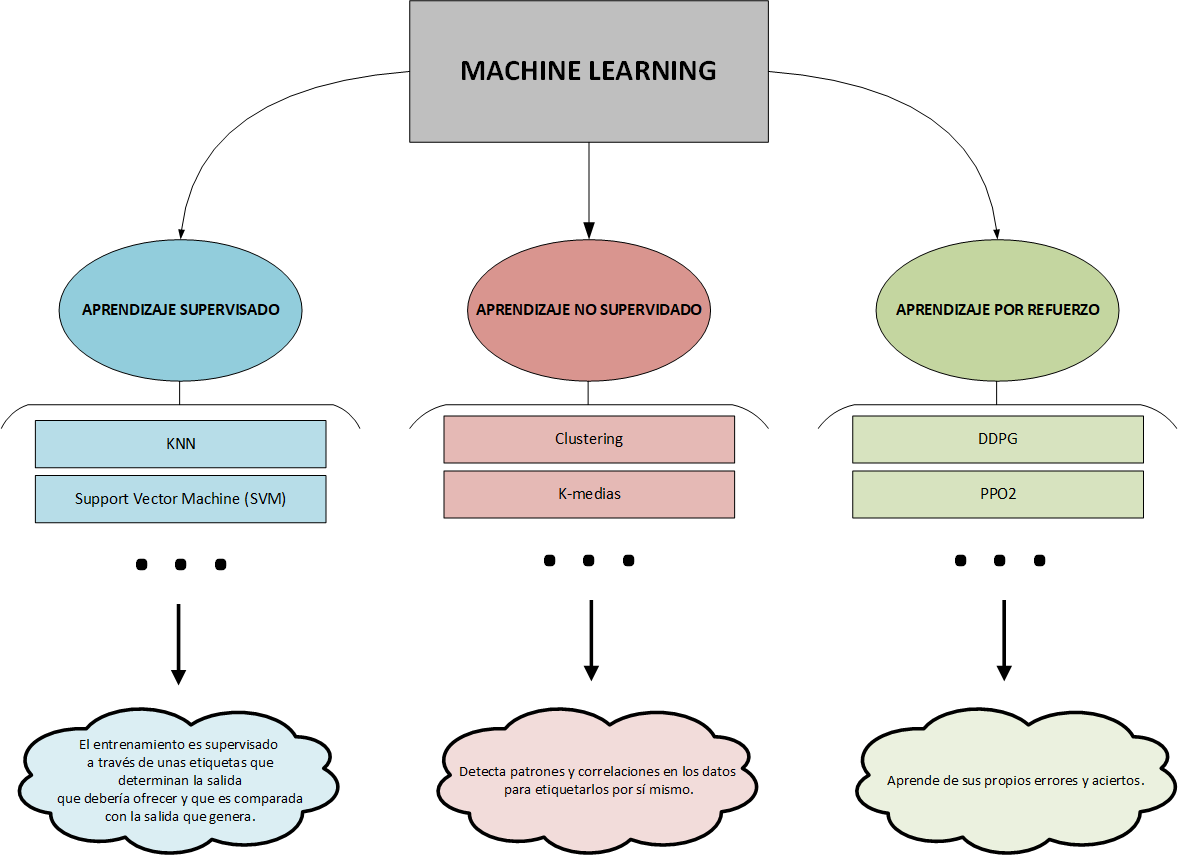
\includegraphics[scale=0.6]{captures/IA2.png}
	\caption{Categorización de tipos de aprendizajes en Machine Learning.}
	\label{fig:IA2} % Unique label used for referencing the figure in-text
	%\addcontentsline{toc}{figure}{Figure \ref{fig:GDS}} % Uncomment to add the figure to the table of contents
\end{figure}

Dentro del Machine Learning y todo lo que esto abarca, existe un conjunto de técnicas concretas que hacen uso de \textbf{redes neuronales artificiales} que se compone de un número de niveles jerárquicos, es lo que se denomina \textbf{Deep Learning}. Hay que decir que, aunque se haga uso de ese nombre, aun desconocemos la forma de trabajar exacta del cerebro humano. \\

Estas técnicas son aproximaciones o ideas generales de como se cree que funciona nuestro desarrollo del razonamiento. Para que se entienda con un ejemplo, aprendimos y nos inspiramos a volar observando los pájaros, aunque los aviones no utilicen exactamente las mismas técnicas que ellos. \\

Estas redes neuronales son adecuadas en determinados problemas en los que no necesitamos saber \textbf{cómo piensa el agente}, simplemente queremos conseguir la \textbf{mejor respuesta} posible, sin más. Son usados cuando se dispone de mucha fuerza de computación y datos no estructurados (reconocimiento de imágenes, por ejemplo). Las redes neuronales pueden funcionar tanto en \textit{aprendizaje supervisado} como en \textit{aprendizaje por refuerzo}. Podemos indicarle los ejemplos con los que se quiere que aprenda y las salidas que debería de dar, o bien permitirle que explore el mismo y evalúe sus propias decisiones una vez obtiene recompensas negativas o positivas como fruto de las mismas, esto dependerá de la naturaleza del problema a resolver y de los datos que deba manejar.\cite{article:deeplearning}\\

Cuando se usa Deep Learning dentro del paradigma de aprendizaje por refuerzo, es llamado \textbf{Aprendizaje por refuerzo profundo} y es una combinación que ha sido demostrada \textbf{muy eficaz} y potente para la resolución de algunos problemas tales como juegos de mesa, videojuegos, etc. \\

\begin{figure}[H]
	\centering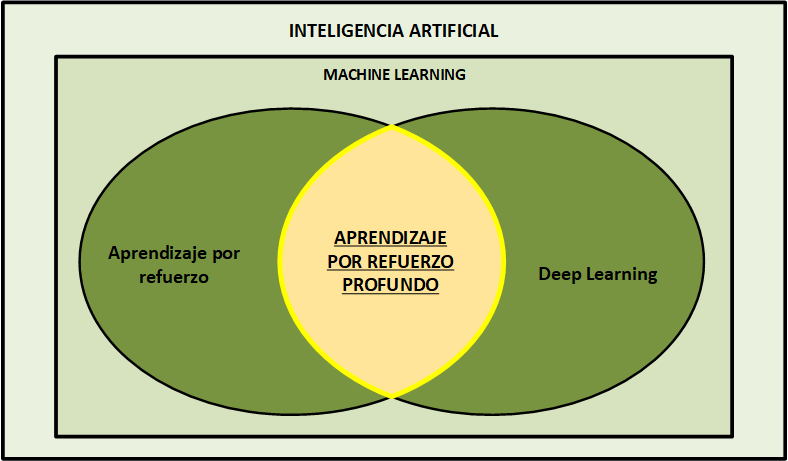
\includegraphics[scale=0.7]{captures/IA.png}
	\caption{Estructura de conceptos dentro de la Inteligencia Artificial.}
	\label{fig:IA} % Unique label used for referencing the figure in-text
	%\addcontentsline{toc}{figure}{Figure \ref{fig:IA}} % Uncomment to add the figure to the table of contents
\end{figure}

Tanto mi tutor, Juan Gómez Romero, como yo, hemos decido investigar de una forma más exhaustiva sobre todo lo que significa el \textbf{Aprendizaje por refuerzo profundo}. Tanto en el Grado de Ingeniería Informática como en el Máster, la información que se aportaba sobre este tema era simplemente un par de frases dando su definición. Nunca hemos abordado o resuelto, tanto de forma teórica como práctica, problemas en los que la mejor metodología que se puede usar dentro del Machine Learning sea esa. Como sí ha ocurrido con AlphaGo o AlphaStar, los cuales serán analizados en este trabajo. Personalmente, me resulta muy interesante a nivel académico debido al total desconocimiento desde el que parto como estudiante y sobre el cual me gustaría avanzar y ver las posibilidades que ofrece.

\section{Motivación}\label{sec:DRL2}

El aprendizaje por refuerzo profundo ha sido demostrado como la mejor tecnología actual para resolver ciertos problemas o, de forma más concreta, algunos juegos y videojuegos competitivos. Son el caso de \textbf{AlphaGo} y \textbf{AlphaStar}, elaborados por la empresa \href{https://deepmind.com/}{DeepMind} de Google.\cite{article:DeepMind} \\

En el caso de AlphaGo, fue capaz de ganar a uno de los mejores, sino el mejor, jugador de GO del mundo actualmente llamado Lee Sedol. Consiguió ganar 4 partidas frente a 1 del campeón mundial.\cite{article:leesedol} \cite{article:leesedol2} \\

En el caso de AlphaStar, supuso un paso más allá en el avance de este campo, creando un agente capaz de colarse entre el 0,2\% de los mejores jugadores del mundo. Se pasó de un problema con tiempo discretizado (por turnos) en el que se conocía en todo momento el entorno completo (conjunto de fichas en juego), a un videojuego en tiempo real (inexistencia de turnos) en el que el jugador solo tienen como entrada de información una porción del entorno (es como ver solo una parte del tablero). Eso sin contar con la complejidad de la información de entrada como conjunto de posibles acciones que se pueden realizar en cada momento.\cite{article:vinyals} \cite{article:vinyals2} \\

En este Trabajo fin de Máster se va a tratar de arrojar algo de luz a este paradigma, prácticamente desconocido a nivel académico. Como se trata de un conjunto de técnicas punteras que aún se están investigando, desarrollando y perfeccionando, este trabajo se va a centrar en explicar de una forma básica las técnicas más comunes que usan empresas como DeepMind, aplicándolas a entornos o problemas más simples para poder experimentar con las mismas.\footnote{Hay que tener en cuenta que estas empresas invierten muchos recursos y tiempo a estas investigaciones, por lo que no se puede abarcar de una forma tan ambiciosa de manera académica, por desgracia.} \\

Una vez hecho esto, vamos a enfocarlo y a tratar de explicar de una forma algo más abstracta cómo funcionan las arquitecturas basadas en aprendizaje por refuerzo profundo de estos agentes que suponen la actual cumbre de este tipo de tecnologías. \\

\section{Objetivos del proyecto}\label{sec:objetivos}

Los objetivos principales que se van a tratar de abordar en este trabajo son: \\

\begin{enumerate}
	\item Entender los \textbf{conceptos principales} de la Inteligencia Artificial, concretamente todo lo relacionado con el aprendizaje por refuerzo. \\
	
	\item Entender, de una forma genérica, el \textbf{funcionamiento y metodología} que siguen las \textbf{técnicas} más importantes de este campo. \\
	
	\item Descubrir las posibilidades que nos da \textbf{gym} \cite{article:gym} para la construcción de \textbf{entornos o simulaciones} en los que entrenar a nuestros agentes sin la necesidad de espacios físicos reales para ciertos problemas. \\
	
	\item Saber aprovechar los recursos en la nube para una mayor eficiencia en los entrenamientos de los agentes, concretamente en la plataforma de \textbf{Google Cloud}. \\
	
	\item Saber aplicar las diferentes técnicas en los distintos entornos mencionados anteriormente y saber ajustarlos al máximo. \\
	
	\item Monitorizar el proceso de aprendizaje y la experiencia obtenida por el agente con la finalidad de validar su progreso y determinar cuando está logrando aprender. \\
	
	\item Analizar, desde el punto de vista científico y técnico, problemas considerados ya resueltos gracias al paradigma de aprendizaje profundo por refuerzo tales como \textbf{AlphaGo} y \textbf{AlphaStar}. \\
	
	\item Tener una visión básica y general del progreso actual en este campo y a lo que podría llegar en el futuro. \\
	
	\item Reflexionar sobre las conclusiones que se pueden extraer del cumplimiento de los objetivos anteriores y considerar posibles mejoras futuras del trabajo realizado durante este proyecto.
\end{enumerate}

\section{Estructura del proyecto}\label{sec:planificacion}

Este proyecto está formado por 11 capítulos repartidos en 5 partes, junto con un apéndice formado por otros 3 capítulos más.

\begin{figure}[H]
	\centering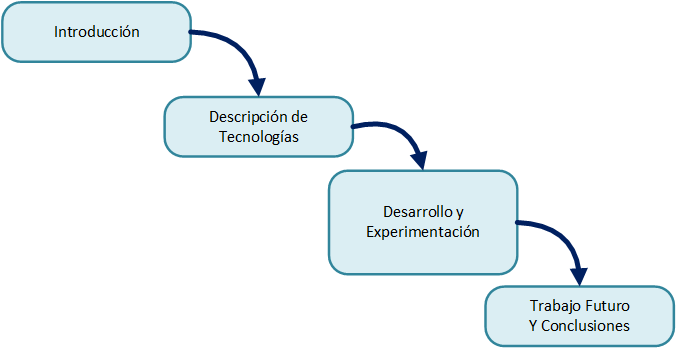
\includegraphics[scale=0.8]{captures/estructuraProyecto.png}
	\caption{Modelo de cascada.}
	\label{fig:estructuraProyecto} % Unique label used for referencing the figure in-text
	%\addcontentsline{toc}{figure}{Figure \ref{fig:IA}} % Uncomment to add the figure to the table of contents
\end{figure}

Estas partes son: \\

\begin{itemize}
	\item \textbf{Introducción}: Se habla del contexto, motivaciones y objetivos que se esperan del proyecto. \\
	
	\item \textbf{Descripción de Tecnologías}: Tecnologías que se combinan y usan para resolver problemas de IA, tales como deep learning(DL), aprendizaje por refuerzo(RL) y la combinación de ambas; aprendizaje por refuerzo profundo(DRL).\\
	
	\item \textbf{Desarrollo y experimentación}: Se trata las herramientas y recuros actuales que existen para aplicar estas técnicas y se analizan los resultados obtenidos en varios entornos seleccionados.\\
	
	\item \textbf{Estado del arte}: Se razonará sobre hasta donde han sido capaz de llegar estas técnicas y qué podemos esperar de ellas en el futuro. Analizando agentes muy novedoso como \textit{AlphaGo} y \textit{AlphaStar}. \\
	
	\item \textbf{Posibles Mejoras y conclusiones}: Se realiza un análisis crítico del trabajo y se exponen las sensaciones y conceptos adquiridos. \\
	
	\item Además, se ha añadido un apéndice con información relevante sobre \textbf{configuración en la nube}, \textbf{uso de la máquina virtual} y \textbf{Stable Baselines} como herramienta alternativa.
\end{itemize}

El planteamiento final del proyecto puede observarse de una forma más detallada en el diagrama de Gantt de la figura \ref{fig:gantt}:

\begin{figure}[H]
	\centering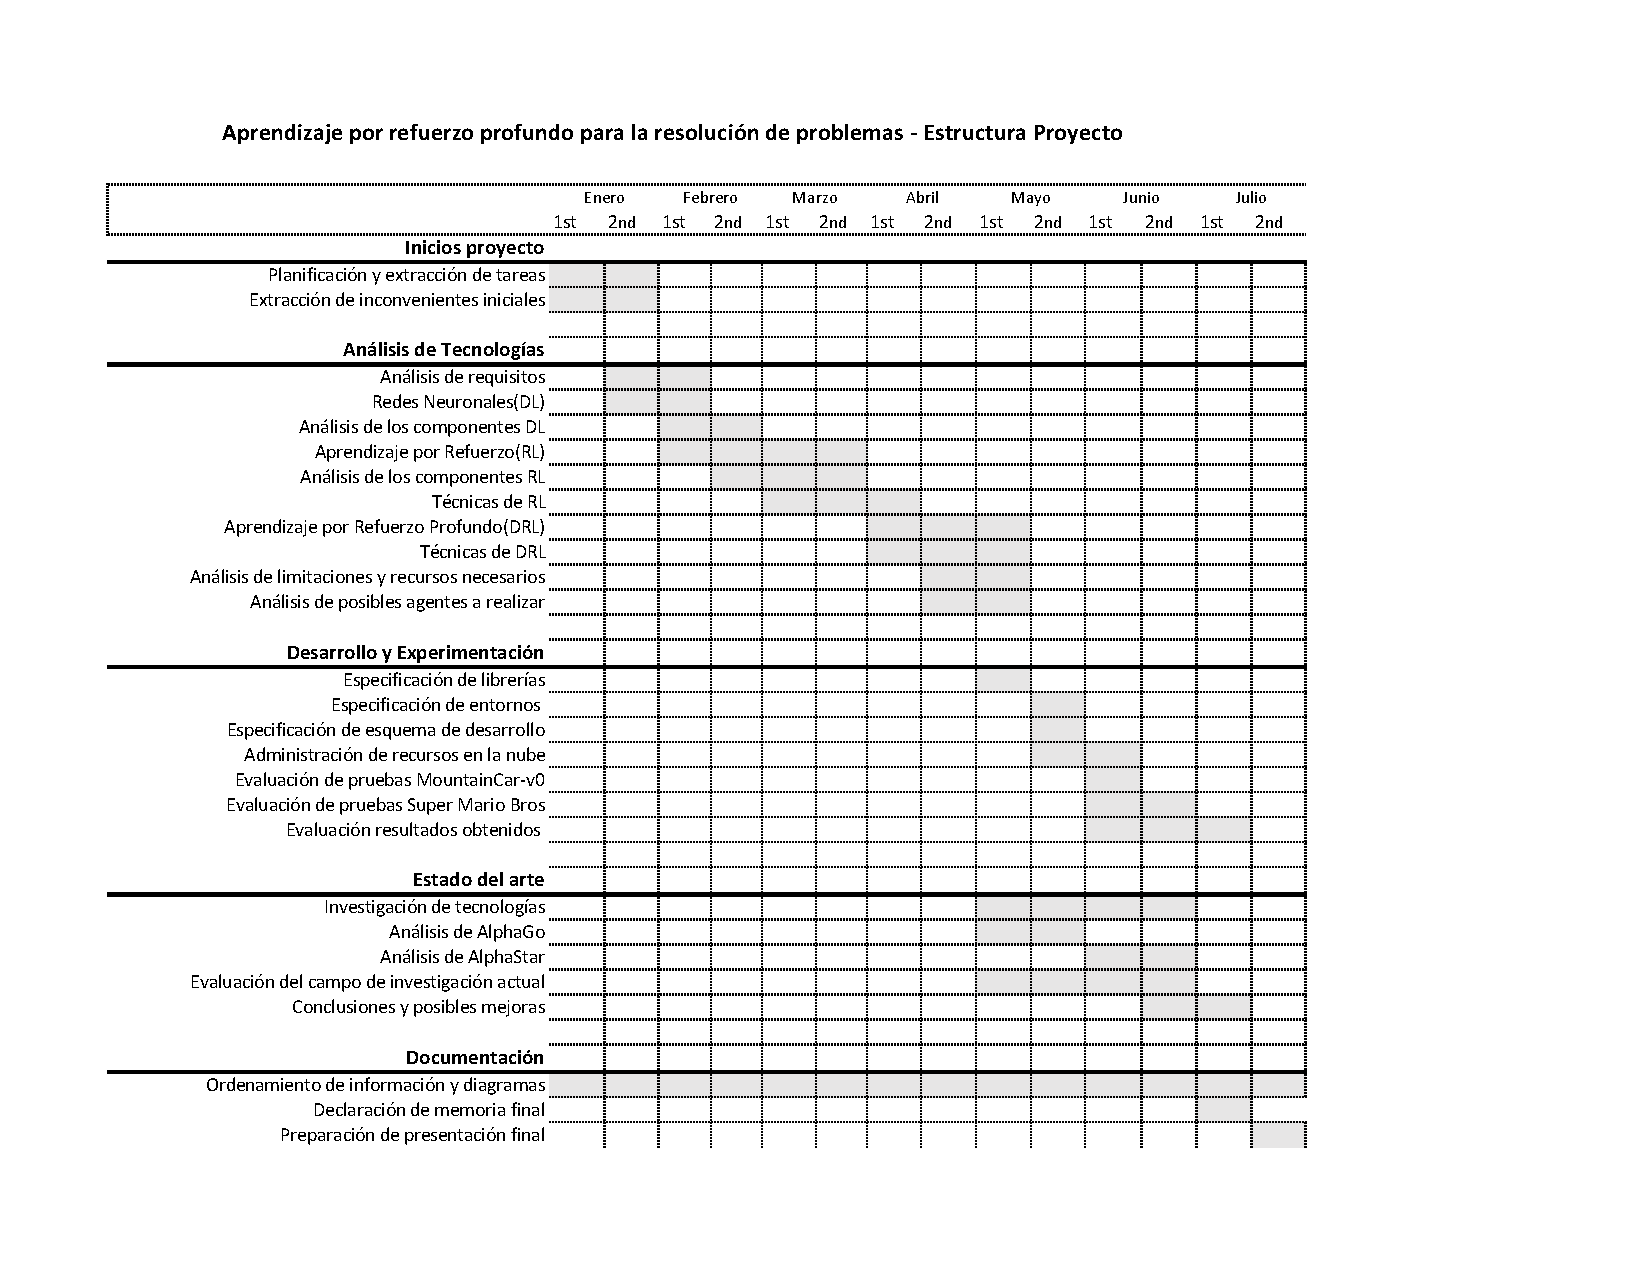
\includegraphics[scale=0.75]{captures/gantt.pdf}
	\caption{Diagrama de Gantt.}
	\label{fig:gantt} % Unique label used for referencing the figure in-text
	%\addcontentsline{toc}{figure}{Figure \ref{fig:IA}} % Uncomment to add the figure to the table of contents
\end{figure}

%----------------------------------------------------------------------------------------
%	PART 2
%----------------------------------------------------------------------------------------

\part{Descripción de Tecnologías}

%----------------------------------------------------------------------------------------
%	CHAPTER 2
%----------------------------------------------------------------------------------------
\section*{Introducción}

En el Grado de Ingeniería Informática de la Universidad de Granada, más concretamente en la especialidad de Computación y Sistemas Inteligentes, así como en el Máster profesionalizante, hemos podido ver y experimentar con las redes neuronales profundas y ver las posibilidades que estas ofrecen. \\

Del mismo modo, hemos podido comprobar que llega un momento en el que estos tipos de agentes se \textbf{``estancan''} en su aprendizaje cuando no alcanzan a resolverlos a la perfección, de tal manera que por más información etiquetada que se le aporte no consigue aprender nada nuevo o, incluso se \textbf{sobreajustan}. Quizás pueden ser mejorados un poco más cambiando la arquitectura de las capas neuronales que utiliza, pero si el modelo ya está bastante bien ajustado se traduce en mucho tiempo de pruebas y cambios para muy poca recompensa en los resultados, si es que se consiguen. \\

En definitiva, esta tecnología para ciertos problemas puede quedarse algo corta o no conseguir aprender lo suficiente como para encontrarse satisfecho con los resultados, como sería el caso de jugar bien a \textbf{Go}. Aunque ya hablaremos de ese tema.\cite{article:go} \\

Se puede entender mejor con el siguiente ejemplo, el cual encuentro muy apropiado ya que la Inteligencia Artificial trata de imitar la metodología del aprendizaje humano. Si queremos ser los mejores jugando al Ajedrez, está bien comenzar a leer libros y analizar partidas de jugadores profesionales; aprender patrones y técnicas comunes así como una noción básica del juego. Esto sería equivalente a las redes neuronales con información supervisada. \\

Sin embargo, los humanos llegan a un punto en el que por más libros que leen o partidas que observan, no son capaces de mejorar más. ¿Por qué ocurre esto? Esos jugadores profesionales que escriben esos libros tienen un conocimiento interno fruto de la \textbf{experiencia} que no es fácil aclarar o expresar en el papel con lenguaje natural(o un dataset, para la red neuronal), es un plus que se adquiere solamente con la \textbf{práctica}. \\

Por ello, los humanos que a parte de ``estudiar'' (aprendizaje supervisado), practican y experimentan posibles situaciones de juego (aprendizaje por refuerzo), pueden llegar a conseguir ese conocimiento extra que los hace únicos y posiblemente mejores que el resto de sus adversarios. \\

Esta es la filosofía y el origen del nacimiento del aprendizaje por refuerzo profundo. Haciendo uso de las redes neuronales para manejar esa experiencia que el agente adquiere a medida que acierta o erra en sus intentos, el agente será capaz de aprender tanto de los aciertos como de los errores que comete e ir actualizándose a versiones mejores de sí mismo de forma autónoma. \\

En esta parte estudiaremos de una forma \textbf{abstracta y teórica} tanto las redes neuronales como los tipos de algoritmos de aprendizaje por refuerzo que utilizaremos para resolver los distintos problemas que se plantearán en el futuro a lo largo de este trabajo. \\

De esta forma iremos adquiriendo los conocimientos y conceptos básicos que necesitaremos para luego entender cómo funcionan en la práctica y cuales son las causas de los buenos y malos resultados que vayamos obteniendo.

\chapterimage{red-neuronal.jpg}
\chapter{Redes Neuronales}\label{sec:deeplearning}

Como hemos mencionado anteriormente, estas técnicas se apoyan firmemente en el uso de las redes neuronales. Son técnicas que ya conocemos del Grado y el Máster respectivamente, aunque considero que no está mal repasarlo de forma resumida. \cite{article:redesNeuronalesMicrosoft} \cite{book:TFGredes} \cite{book:berzal} \cite{article:redesNeuronales} \cite{article:RLromero} \\

\begin{figure}[H]
	\centering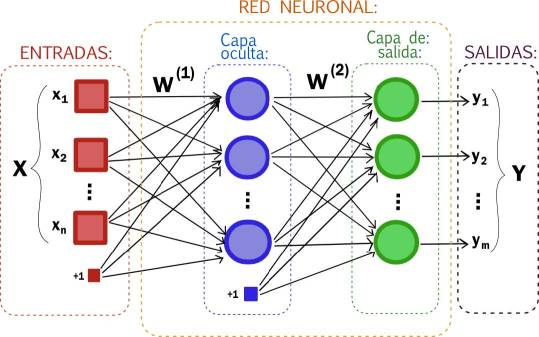
\includegraphics[scale=1]{captures/redNeuronal.jpg}
	\caption{Esquema simplificado de una red neuronal. \cite{article:redNeuronal}}
	\label{fig:redNeuronal} % Unique label used for referencing the figure in-text
	%\addcontentsline{toc}{figure}{Figure \ref{fig:redNeuronal}} % Uncomment to add the figure to the table of contents
\end{figure}

Las redes neuronales están formadas por un conjunto de nodos (neuronas), que están conectadas entre sí, tal y como podemos ver en la figura \ref{fig:redNeuronal}, por ejemplo. \\

Estos nodos se encuentran organizados por \textbf{capas}. La \textbf{primera capa} está asociada a la entrada o \textit{input}, la \textbf{última capa} a la salida que devuelve la red y el resto de capas que se encuentran entre la primera y la última son conocidas como \textbf{capas ocultas o intermedias}. \\

La entrada es un \textbf{vector de características} del problema que queremos resolver. Por ejemplo, si estamos intentando decidir el siguiente movimiento a realizar en un tablero de ajedrez, el vector de características estaría formado por elementos que indicasen la pieza que hay en cada casilla respectivamente (o indicar que no hay ninguna). Es un ejemplo, ya que no sería la única manera de describir el tablero para una red neuronal. Por tanto, la capa de entrada tendrá tantas neuronas como elementos el vector de características; cada neurona recibe una de las características consideradas. \\

Las capas ocultas, pudiendo ser una o más capas, no tienen una conexión directa con el entorno como hemos visto anteriormente. En su lugar, la entrada que recibe es la salida de la capa anterior(capa de entrada en este caso). La salida que devuelvan los nodos de esta capa serán utilizados como entrada en la capa siguiente. ¿Para que sirve esto? La repuesta resumida es que si solo tuviéramos la capa de entrada y salida, las entradas serían demasiado independientes entre sí a la hora de influir en la salida seleccionada entre todas las posibles. En general, los problemas del mundo real son mucho más complejos que eso y es necesario que la red sea capaz de detectar patrones e interdependencias entre los distintos valores de las entradas. Estas capas ocultas ayudan a dar esa \textbf{riqueza} al proceso.\cite{article:redNeuronal2}\\

La capa de salida recoge los datos de la última capa oculta y los procesa para dar una respuesta definitiva en la red. La forma en la que da esta salida depende de diversos factores de la propia capa que veremos un poco más adelante. \\

Las conexiones de los nodos de una capa a otra son definidos por los \textbf{pesos}($w_i$). Estos pesos son utilizados por los nodos para dar la salida siguiente, tal y como se ve en la figura \ref{fig:redNeuronal}.

\section{Funciones de activación(h)}\label{sec:activacion}

Cada neurona no transmite la entrada que recibe a las siguientes de forma directa. Antes de hacer esto, procesa dicha entrada. Esto se realiza mediante la \textbf{función de activación}. Estas pueden ser de muchos tipos y determina cuando la neurona se \textbf{excita o no} en función de las entradas que recibe junto con su ponderación (ya que su entrada se compone de las salidas de las neuronas de la capa anterior)\cite{article:redNeuronal2}. \\

Se han propuesto muchos tipos de funciones de activación en este campo, vamos a mencionar las más habituales o las que más hemos utilizado durante la carrera y el Máster: \\

\begin{itemize}
	\item \textbf{Sigmoide}: Las neuronas sigmoide se comportan sumando todas las entradas ponderadas, es decir, aplicándoles sus respectivos pesos, para luego utilizar ese único valor (z) de la siguiente forma: 
	\begin{equation*}
	\sigma(z) = \frac{1}{1+e^{-z}}
	\end{equation*}
	
	Se hace de esta manera para que dicha función tenga la siguiente forma, si la dibujamos en un plano bidimensional:
	
	\begin{figure}[H]
		\centering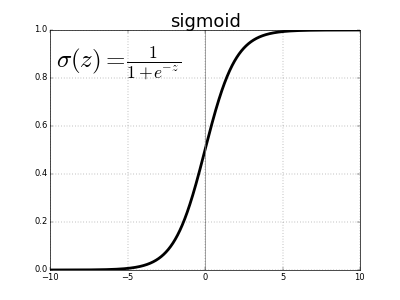
\includegraphics[scale=0.5]{captures/sigmoide.png}
		\caption{Función sigmoide en plano bidimensional. Extraída de origen \cite{article:redNeuronal2}.}
		\label{fig:sigmoide} % Unique label used for referencing the figure in-text
		%\addcontentsline{toc}{figure}{Figure \ref{fig:sigmoide}} % Uncomment to add the figure to the table of contents
	\end{figure}

	En la figura \ref{fig:sigmoide}, vemos como la salida se acota entre los valores 0 y 1 independientemente de las entradas que pueda recibir. El valor neutro de la entrada z(valor 0), corresponde con un valor intermedio de la salida(valor 0,5). A medida que la entrada es positiva y más alta, la salida se acerca al valor 1, mientras que cuando la entrada es negativa y menor, la salida se acerca al valor 0. \\
	
	Esto hace que no haya tanta diferencia entre un conjunto de entradas muy altas a otras que no lo son tanto, por ejemplo, ya que en cualquier caso al ser valores positivos la neurona se va a excitar y devolver un 1. Lo mismo ocurre para las entradas negativas y la salida 0. \\
	
	\item \textbf{Rectified linear unit}(ReLU): Esta función es actualmente más usada que la sigmoide. Principalmente se debe a a la existencia de más capas en las redes neuronales. Los pesos de las neuronas sigmoide son mucho más difíciles de actualizar debido al \textbf{problema de desaparición del gradiente}, aunque no vamos a entrar en detalles con eso. La función es:
	
	\begin{equation*}
	R(z) = max(0,z)
	\end{equation*}
	
	Esta función es más sencilla de entender incluso que la anterior. Básicamente si el valor de la sumas ponderadas de las entradas es menor que 0, se devuelve el valor 0. Si esa suma ponderada de entrada es positiva, se devuelve tal cual:
	
	\begin{figure}[H]
		\centering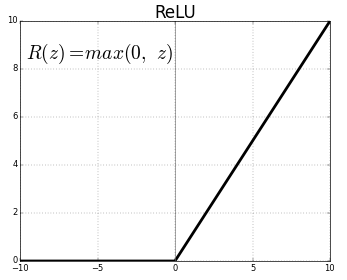
\includegraphics[scale=0.5]{captures/relu.png}
		\caption{Función ReLU en plano bidimensional. Extraída de origen \cite{article:redNeuronal2}.}
		\label{fig:relu} % Unique label used for referencing the figure in-text
		%\addcontentsline{toc}{figure}{Figure \ref{fig:relu}} % Uncomment to add the figure to the table of contents
	\end{figure}
\end{itemize}

En general, se utilizan estos tipos de funciones no lineales debido a que permiten que las redes detecten esas relaciones no lineales entre entradas y salidas. Cosa que es muy frecuente a la hora de resolver todo tipo de problemas en nuestro día a día (clasificación de dígitos manuscritos, por ejemplo). La mayoría de problemas que podemos resolver con estas técnicas no se van a ajustar bien a funciones lineales, hay que tenerlo siempre en cuenta.

\section{Funciones de salida (h')}\label{sec:funcionsalida}

Las funciones de salida son utilizadas en la \textbf{última capa de la red neuronal}. Tratan de utilizar los valores que han llegado a este punto de la red y transformarlos en una \textbf{respuesta final} al problema que está tratando de resolver. La más frecuente y una de las más utilizadas es la \textbf{función exponencial normalizada o softmax}. Suele ser utilizada en problemas de clasificación con salidas discretas, ya que podemos obtener una \textbf{distribución de probabilidades} entre las posibles salidas:

\begin{equation*}
\sigma(z)_j = \frac{e^{z_j}}{\sum^K_{k=1}e^{z_k}}
\end{equation*}

Para j con valores entre 1 y K. La idea, para este tipo de problemas con un número limitado de salidas posibles,  es que la última capa de la red neuronal tenga tantos nodos o neuronas como posibles salidas. Cada neurona representaría una posible respuesta de la red y el valor que devuelve cada una de ellas sería la probabilidad de que la respuesta que representa sea la correcta. \\

La potencia de esto es que la red neuronal no solo aporta una salida(aquella neurona con valor más alto), sino que indica una distribución de probabilidades de todas ellas. 

\section{Funciones de coste}\label{sec:funcioncoste} 

Es muy posible, y sobretodo durante el proceso de aprendizaje, de que la red neuronal se \textbf{equivoque} al dar una salida para una entrada determinada. Hay que buscar un modo de comparar la salida dada por la red de la salida real o salida que debería haber dado. \\

Las \textbf{funciones de coste o de pérdida} son utilizadas una vez la red neuronal da una salida definitiva. Trata de evaluar o, mejor dicho, cuantificar el error que ha tenido. Hay muchas formas de analizar o evaluar este error, cada una con sus pros y contras, vamos a ver un par de ellas:\\

\begin{itemize}
	\item \textbf{Error cuadrático medio}(MSE): Mide el promedio de los errores al cuadrado. En otras palabras, la diferencia de el valor que debería estimar de lo que estima realmente:
	
	\begin{equation*}
	MSE = \frac{1}{n} \sum_n^{j=1}{(d_j - y_j)^2}
	\end{equation*}
	
	Siendo n el número de salidas que ha dado, \textit{d} las predicciones e \textit{y} las salidas correctas. Esta función tiene el inconveniente de que los errores más altos afectan mucho al promedio. \\
	
	\item \textbf{Entropía cruzada}: Es un cálculo que consiste en la suma negativa del producto del logaritmo de cada componente de las salida predicha y el componente de las salida real que debería dar:
	
	\begin{equation*}
	H(p,q) = -\sum_x p(x)log(q(x))
	\end{equation*}
	
\end{itemize}

El objetivo de cualquier red neuronal debe ser el de \textbf{minimizar} esta función de pérdida, ya que es sinónimo de una mayor frecuencia de acierto en las salidas que aporta. Dicho de otra manera, el objetivo es buscar la combinación de pesos en la red que hagan que las salidas en la función de error sea la mínima posible de forma general para cualquier caso que se le plantee. \\ 

\textbf{Decidir} una función de pérdida es \textbf{muy importante} a la hora de entrenar la red en un futuro, ya que dependiendo de su diseño puede hacer más difícil su optimización o menos(por tanto, que lleguemos a un conjunto de pesos determinado para la red u otros diferentes). Dependiendo de la naturaleza del problema que queramos resolver y de cómo se interpreta la entrada para la red. \\

Esta es una de las tareas del programador, no solo saber un lenguaje de programación, sino decidir y probar aquellas cosas en las que tienen un motivo para creer que pueden funcionar mejor que otras.

\section{Algoritmos de optimización}\label{sec:optimizacion}

Hasta ahora, todo lo que se ha explicado de las redes neuronales es diseñado y establecido de antemano (las capas, número de neuronas por capa, las funciones de activación y salida que van a tener, función de coste, etc). Solo hay una cosa que va a variar en dichas redes neuronales a lo largo de su aprendizaje: \textbf{la actualización de sus pesos} en las conexiones entre sus respectivas capas. \\

Los \textbf{algoritmos de optimización} buscan concretamente esto. Usando los valores de error que devuelve la función de perdida, determina como se van a actualizar los pesos con la finalidad de que la red neuronal mejore en sus cálculos de salidas futuras. De nuevo, hay muchos algoritmos para realizar esta tarea, algunos de ellos son: \\

\begin{itemize}
	\item \textbf{Gradiente descendente Estocástico}: Es una técnica genérica que sirve para minimizar cualquier función. Con el uso de derivadas, es capaz de encontrar la combinación de pesos óptima o muy buena para devolver el mejor punto de esa función. \\
	
	El principal problema aquí es que estamos hablando de redes neuronales que pueden tener cientos de miles de parámetros, por lo que no es viable hacer este tipo de cálculos a lo largo del tiempo. \\
	
	Por ello, esta técnica se diferencia del gradiente descendente tradicional en que utiliza solo una muestra aleatoria de todo el conjunto de entradas en cada iteración para actualizar los pesos en la función de perdida. Esto mete algo de aleatoriedad en el aprendizaje y evita sobreajuste y estancamiento en el proceso. Además, también se puede incluir una organización de estas muestras en \textbf{mini lotes} (mini batches), haciendo el entrenamiento aún más rápido al tener la posibilidad de paralelizar estas operaciones.
	
	\begin{figure}[H]
		\centering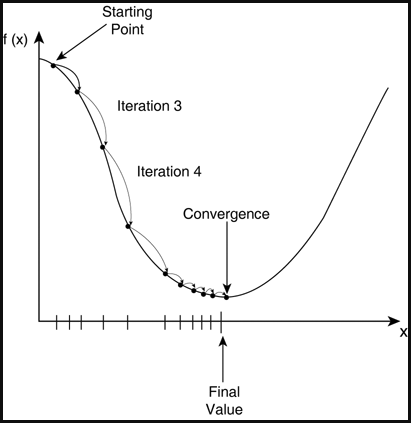
\includegraphics[scale=0.5]{captures/gds.png}
		\caption{Ejemplo de proceso de gradiente descendente estocástico en una función f de un solo parámetro. Imagen extraída de origen \cite{article:ejemploGDS}.}
		\label{fig:GDS} % Unique label used for referencing the figure in-text
		%\addcontentsline{toc}{figure}{Figure \ref{fig:GDS}} % Uncomment to add the figure to the table of contents
	\end{figure}

	Si observamos la figura \ref{fig:GDS}, vemos que es un ejemplo muy sencillo. Debemos tener en cuenta que sólo tiene un parámetro (x). El caso es que en redes neuronales tenemos una función que puede tener cientos de miles de parámetros, dependiendo de la red, y que esto ni siquiera es mostrable en una gráfica ya que espacialmente no entendemos más allá de tres dimensiones (2 parámetros más el valor de salida). Por eso es importante el muestreo de entradas, para hacerlo viable computacionalmente. \\

	\item \textbf{Adam}: El algoritmo Adam (Momentum Adaptable) es uno de algoritmos de optimización más usados. No vamos a entrar en detalle, simplemente decir que esta basado en gradientes de primer orden, es computacionalmente eficiente, pocos requisitos de memoria y es muy adecuado para problemas de redes con un gran número de parámetros y datos.  \\
\end{itemize}

En definitiva, las redes neuronales son tan amplias como artículos tiene publicados al respecto y experimentos se han realizado desde su aparición. Solo se pretende dar una vista general de su arquitectura y como funcionan. 

\section{Redes Neuronales Convolucionales(CNN)}\label{sec:convolucional}

Las redes neuronales convolucionales(CNN) son muy similares a las redes ordinarias. De hecho, se pueden entender como una extensión de éstas. Definimos a las redes neuronales vistas hasta este punto como la parte \textbf{densa}. De ellas no se puede saber la metodología de razonamiento, sólo la calidad de los resultados que ofrecen, por lo que es complicado predecir un comportamiento de estas redes. \\

En las redes convolucionales, se supone que las entradas que recibe son directamente imágenes, por ejemplo, en el reconocimiento de dígitos manuscritos. Este tipo de redes mejoran el tratamiento de estos datos, tanto en rendimiento como en calidad de las respuestas. \\

Una imagen tiene una dimensión predeterminada, supongamos por ejemplo 800x800. Esto supone un total de 640000 elementos en el vector de características para cada muestra, eso asumiendo que la imagen es en escala de grises. Si es a color, cada pixel tiene una tripleta de valores RGB, lo que supone $640000*3=1920000$ valores por muestra de entrada. Contar con tantos parámetros desde la capa de entrada ya supone un gran límite para la red, existiendo mayor facilidad y tendencia al sobreajuste. \\

La parte \textbf{convolucional} de la red puede ser entendida como una etapa de \textbf{preprocesamiento} de las imágenes para extraer las características más importantes de las mismas, y estas son las que llegarían a la parte \textbf{densa} de la red, como se estaba mencionando anteriormente. \\

Vamos a ver de forma resumida las distintas capas que constituyen esta parte convolucional de la red.

\subsection{Capa convolucional}\label{sec:convolucional2}

Estas capas realizan un proceso llamado \textbf{convolución}. Reciben la imagen como entrada y luego aplica sobre ella un \textbf{filtro} o \textbf{kernel} que nos devuelve una matriz de datos, como la imagen, solo que con una características concretas destacadas. Por ejemplo, un filtro puede ser usado para la detección de bordes de una imagen únicamente. \\

Ese filtro tiene una \textbf{dimensión}(5x5, por ejemplo) lo cual hace que esos mapas de características mencionados reduzcan la cantidad de parámetros(dimensión de la matriz).\\

Una capa convolucional, a su vez, puede tener más de un filtro, lo que se conoce como \textbf{canales}(channels) del mapa de características. La idea es que cada filtro detecte características específicas de la imagen(bordes, patrones, etc).

\begin{figure}[H]
	\centering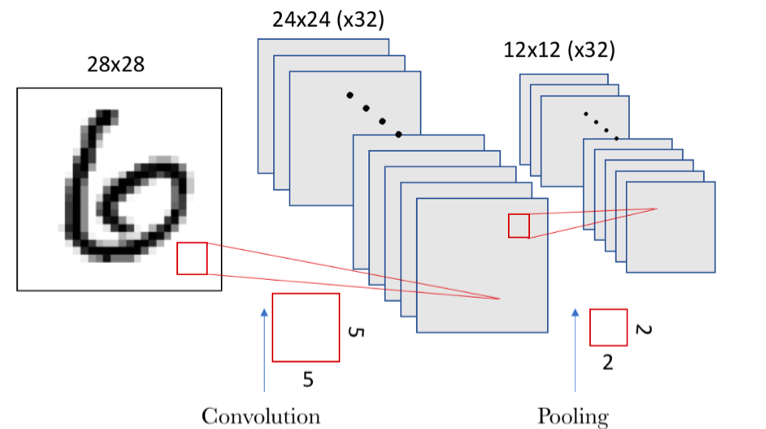
\includegraphics[scale=0.5]{captures/convolucional.png}
	\caption{Aplicación de capa convolucional a imágen de entrada.}
	\label{fig:convolucional} % Unique label used for referencing the figure in-text
	%\addcontentsline{toc}{figure}{Figure \ref{fig:GDS}} % Uncomment to add the figure to the table of contents
\end{figure}

En la figura \ref{fig:convolucional}, tendríamos 32 filtros 5x5 diferentes, dado que obtenemos 32 matrices 24x24 a partir de una sola imagen 28x28.

\subsection{Capa de reducción o Pooling}\label{sec:pooling}

Esta capa suele situarse siempre inmediatamente después de una capa convolucional, aunque también es posible realizar más de una capa pooling seguida. Su utilidad, en resumen, consiste en reducir las dimensiones de los mapas de características que se mencionaban anteriormente aún más. Irremediablemente, al realizar este proceso, se pierde información por el camino. Aunque el sentido común pueda determinar en un principio que esto es negativo, generalmente es positivo. \\

La disminución en el tamaño o dimensión de los mapas de características produce una reducción de sobrecarga en el cálculo en las capas venideras, haciendo viable el procesamiento de imágenes con una resolución mayor. Además, es una representación más \textbf{genérica} del problema que se trata de resolver, por lo que implícitamente reduce la tendencia al sobreajuste por parte de la red. \\

Hablando sobre la operación de reducción concretamente, se suele dividir la imagen en \textit{submarcos} o un conjunto de rectángulos. En cada una de estas \textit{subzonas}, se suelen utilizar la operación de \textbf{Max-Pooling}, la cual quiere decir que nos quedamos con el valor más alto, como se aprecia en la figura siguiente:

\begin{figure}[H]
	\centering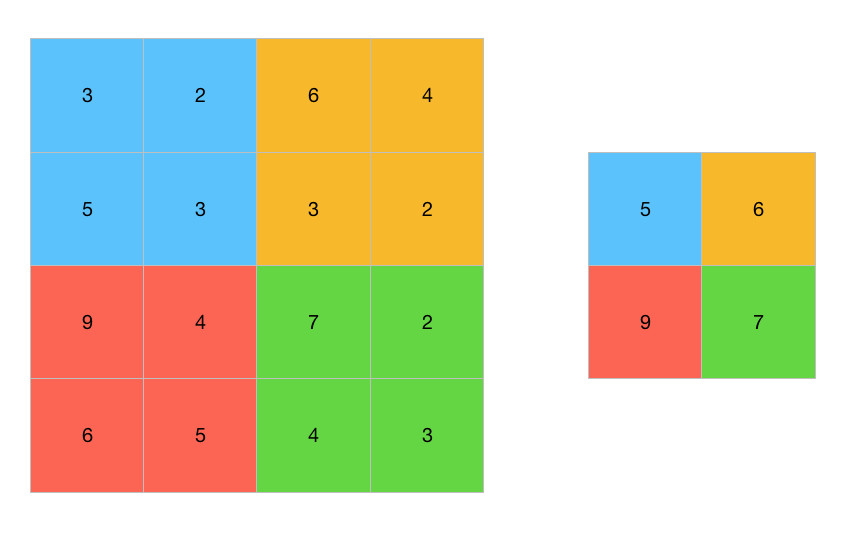
\includegraphics[scale=0.5]{captures/pooling.jpg}
	\caption{Aplicación de capa Max-Pooling a mapa de características.}
	\label{fig:pooling} % Unique label used for referencing the figure in-text
	%\addcontentsline{toc}{figure}{Figure \ref{fig:GDS}} % Uncomment to add the figure to the table of contents
\end{figure}

\subsection{Capa Flatten}\label{sec:flatten}

Una vez la imagen haya sido tratada en sucesivas capas convolucionales y Pooling, cada vez tendremos más canales de menor dimensión con características más aisladas y específicas del problema. Solo queda conectarla con la parte densa, para tratar esas características como veíamos anteriormente; capa de entrada, capas ocultas o intermedias y las capa de salida. ¿Cómo podemos juntar estas partes? \\

Ese es el propósito de la \textbf{capa Flatten}. Explicado de forma simple, coge todas las características y las concatena en un único \textbf{vector de características}. La capa de entrada de la parte densa tendrá una neurona por cada una de estas características.

\begin{figure}[H]
	\centering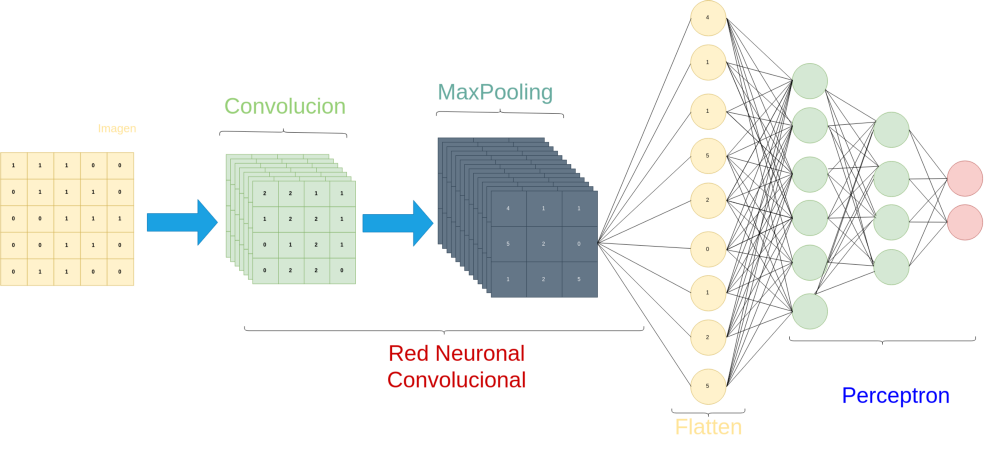
\includegraphics[scale=0.5]{captures/flatten.png}
	\caption{Adaptación de parte convolucional a parte densa con uso de capa Flatten.}
	\label{fig:flatten} % Unique label used for referencing the figure in-text
	%\addcontentsline{toc}{figure}{Figure \ref{fig:GDS}} % Uncomment to add the figure to the table of contents
\end{figure} 


\chapterimage{RL.jpg}
\chapter{Aprendizaje por refuerzo(RL)}\label{sec:RL}

También es muy importante tener conocimientos con respecto a las técnicas de aprendizaje por refuerzo(RL) para desarrollar los algoritmos que veremos y utilizaremos más adelante. Comenzaremos por explicar los fundamentos del RL, los componentes que lo forman y definen un problema de este tipo, junto con algunos de sus conceptos básicos y metodología genérica, para luego centrarnos en algunas de las técnicas y estrategias más utilizadas y populares en la actualidad. \\

El mundo es muy \textbf{complejo} y los retos que nos plantea también, a veces incluso más de lo que imaginamos. Cuando tratamos de llevar esos problemas al RL, nos encontramos con agentes que deben aprender en entornos con un espacio de estados y posibles acciones muy grande. \\

La metodología de aprendizaje es \textbf{secuencial}. En muchos de los problemas que existen hay consecuencias en las decisiones que no se manifiestan inmediatamente, se demoran en el tiempo. Esto hace que sea complicado definir cómo de buena o mala es una decisión y es uno de los principales retos del RL. \\

Debemos ser conscientes de que siempre tendremos que lidiar con la \textbf{incertidumbre}, es algo inevitable. Los problemas son tan complejos que es imposible tener todos los casos posibles en cuenta de manera específica. Esa incertidumbre es la que da sentido a la \textbf{exploración}, tratando de buscar el equilibrio con la \textbf{explotación} para ofrecer respuestas de la mejor calidad posible en un rango de tiempo viable.\\

Explicaremos todos los conceptos y componentes que conforman los problemas a partir de un marco de trabajo matemático llamado \textbf{Procesos de Decisión de Markov(MDPs)}. El cual nos permitirá modelar virtualmente cualquier problema complejo de una forma que los agentes de RL puedan interactuar y aprender a resolverlos. \cite{book:miguel} \cite{article:RLromero} \cite{book:barto}  \\ 

%Una de las ventajas que tiene el paradigma del aprendizaje por refuerzo es que desarrollan algoritmos \textbf{genéricos}, con una abstracción alta de los problemas a resolver. Esto quiere decir que una misma técnica puede ser utilizada para entrenar dos agentes que resuelven dos problemas totalmente diferentes. Teniendo en cuenta y cambiando antes algunos parámetros para cada uno de ellos, como por ejemplo el formato del input que reciben del entorno, las acciones posibles que pueden realizar, el formato de la experiencia recolectada, el sistema de recompensas, etc. \\

\section{Componentes del RL}\label{sec:componentesRL}

Los dos principales componentes del RL son el \textbf{entorno} y el \textbf{agente}. El entorno es una representación del problema planteado, el agente es un tomador de decisiones, y por tanto, una solución. Una de las diferencias más distintivas que tiene RL con otras técnicas de Machine Learning es que el agente \textbf{interactúa}, tratando de influenciar el entorno realizando \textbf{acciones}, mientras que el entorno \textbf{reacciona} ante ellas, generando nuevos \textbf{estados}. \\

\begin{itemize}
	\item El espacio de estados, el conjuntos de todos los posibles que existen, puede ser finito o infinito dependiendo del problema que sea. Cada estado estará formado por un número \textbf{finito} de variables que lo describe, siempre debe ser finito. \\
	
	\item El espacio de acciones puede variar de un estado a otro, a ese subconjunto se denota como $A(s)$ siendo $s$ el estado del entorno en ese momento. Esto sucede debido a la existencia de problemas en los que, dado un estado, hay acciones que sencillamente no se pueden realizar en ese momento por el agente. Por ejemplo, en ajedrez no es posible mover una pieza mientras que se está en jaque, a no ser que ese movimiento revierta ese estado de amenaza por parte del oponente. El conjunto de acciones también puede ser finita o infinita, pero cada una de ellas está compuestas por una o más variables finitas, igual que los estados.
\end{itemize}

\begin{figure}[H]
	\centering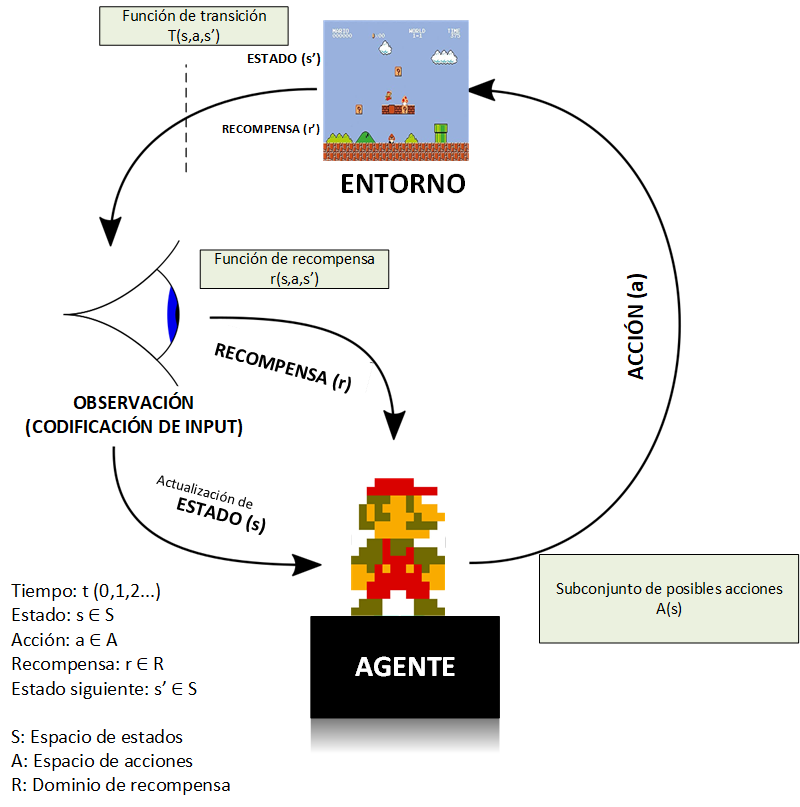
\includegraphics[scale=0.65]{captures/esquemaRL.png}
	\caption{Esquema de componentes del RL. Imagen extraída y posteriormente modificada de origen \cite{article:RLwikipedia}.}
	\label{fig:esquemaRL} % Unique label used for referencing the figure in-text
	%\addcontentsline{toc}{figure}{Figure \ref{fig:GDS}} % Uncomment to add the figure to the table of contents
\end{figure}

Cuando el entorno reacciona, quiere decir que se produce un cambio que, a su vez, repercute en observaciones diferentes por parte del agente en el futuro. La \textbf{recompensa} es una parte fundamental en esta representación, dependiendo de la calidad de esa estimación, el agente realizará un mejor aprendizaje de su propia experiencia. La secuencia que se produce entonces a partir del esquema de la figura \ref{fig:esquemaRL} sería:

\begin{equation*}
S_0, A_0, R_1, S_1, A_1, R_2, S_2, A_2, R_3, ...
\end{equation*}

Es común representar malas acciones con un valor negativo en la recompensa. Entonces, conceptualmente, se trataría de una \textbf{penalización} en su lugar. Sin embargo, la comunidad de RL siempre utiliza la palabra recompensa para definir tanto las buenas decisiones como las malas, refiriéndose directamente a su valor numérico. \\

En la comunidad de RL también se suele utilizar estado del entorno y observación como conceptos intercambiables. Sin embargo, tiene un detalle que puede establecer una diferencia entre ambos conceptos. La \textbf{observación} es una interpretación del estado. Dependiendo del problema, es posible que el agente solo pueda interpretar una parte del estado, que sería lo que ocurre con AlphaStar, por ejemplo. \\

Cuando el agente realiza una acción de su espacio de acciones, puede desencadenar una reacción por parte del entorno que haga cambiar su estado entre su espacio de estados. La función que es responsable de esta \textbf{transición} es llamada \textbf{función de transición}. \\

Después de esa transición, el entorno ofrece un nuevo estado, que indica una nueva observación del agente. El entorno también puede ofrecerle una señal de \textbf{recompensa}. La función encargada de esto es la \textbf{función de recompensa}. \\

Las funciones de transición y recompensa son las que establecen el \textbf{modelo} del entorno como tal. Es importante tener estos conceptos claros antes de continuar, dado que es el marco a partir del cual representaremos cualquier problema para poder entrenar y formar cualquier modelo. \\

%Veremos y entenderemos mejor esto cuando llevemos estas técnicas a la práctica, pero es muy importante mencionar esta gran ventaja. Una vez hemos definido una técnica de aprendizaje, puede ser utilizada casi directamente en cualquier problema para analizar los resultados que adquiere el agente. Obviamente, cada técnica podrá dar mejores o peores resultados dependiendo de los problemas en los que se apliquen claro. \\

%Un factor que tenemos que tener muy claro es que el aprendizaje por refuerzo no esta pensado para \textbf{crear una inteligencia artificial} del tipo que sea. Encaja mejor en la idea de \textbf{mejorar una inteligencia artificial} ya existente. \\

\subsection{Ciclo de interacción}\label{sec:episodios}

%Normalmente un entorno tiene un \textbf{objetivo} bien definido. Ese objetivo esta plasmado de forma implícita en la señales de recompensa.

Las interacciones entre el agente y el entorno se produce en una serie de ciclos secuenciales, tal y como se aprecia en la figura \ref{fig:esquemaRL}. Cada uno de esos ciclos recibe el nombre de \textbf{time-step}. Es una unidad de tiempo en la que se completa cada ciclo de interacción, el cual depende del problema específico. \\

En cada \textit{time-step}, el agente observa el entorno, realiza una acción y recibe una nueva observación y recompensa. La experiencia recolecta estos datos precisamente; siendo el conjunto de observación, acción, recompensa y nueva observación una \textbf{tupla de experiencia}. Más adelante hablaremos de este tema con mayor detenimiento. \\

Los \textbf{episodios} pueden entenderse como cada intento de cumplir el objetivo final. Por ejemplo, si hablásemos de AlphaGo; el agente que juega a GO, un episodio correspondería a una partida completa contra su oponente. \\

Definido de una manera más formal, un episodio es una secuencia de estados del entorno, acciones realizadas y recompensas obtenidas que finalizan con un \textbf{estado terminal}. Ya sea fracasando o teniendo éxito en su objetivo. Un agente puede tardar uno o más episodios en aprender una tarea concreta o conocimiento que le ayude a completar su objetivo. También puede darse el caso de que se tenga que definir un \textbf{problema continuo} el cual no tenga estado terminal. Para ese caso deberemos simular un estado terminal que normalmente se establece limitando un \textbf{máximo} de \textit{time-steps}, veremos esto con detenimiento un poco más adelante también. \\

La sumatoria de todas la recompensas habiendo finalizado un episodio es denominado \textbf{recompensa acumulada} y con ella puede saberse de forma implícita si ha conseguido un estado terminal favorable o no para el agente. Por ejemplo, si la recompensa acumulada es positiva o negativa, aunque no sería la única forma y depende de la definición del problema concreto en el marco MDPs. \\

%Igual esto debería ir en otro lado??????????
%Estos episodios se repiten en la \textbf{fase de entrenamiento} del agente una y otra vez, tratando de recolectar experiencia de juego para mejorarse a sí mismo. La arquitectura de este paradigma se describiría de la siguiente forma: \\
%
%\begin{enumerate}
%	\item El agente realiza acciones con el entorno hasta llegar a un estado terminal, es decir, \textbf{realiza un episodio}. \\
%	\item Recolecta información(\textbf{experiencia}) durante el proceso. \\
%	\item \textbf{Entrena}. Modifica su comportamiento utilizando de algún modo concreto toda esa experiencia adquirida, dependiendo del \textbf{algoritmo de aprendizaje} utilizado. Se puede recolectar experiencia de más de un episodio. \\
%	\item \textbf{Evalúa} si ha conseguido mejorar realmente al actualizarse con esa experiencia. \\
%	\item Se \textbf{actualiza} en caso de que la evaluación determine que es mejor que antes. \\
%	\item \textbf{Repite} todo el proceso. \\
%\end{enumerate}
%
%\begin{figure}[H]
%	\centering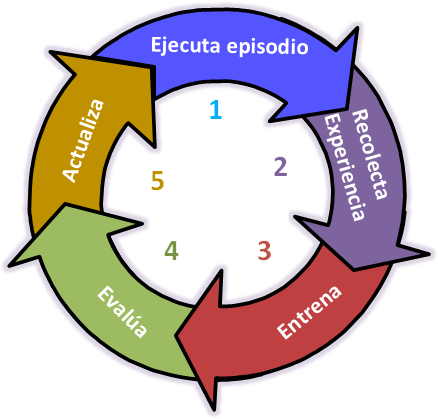
\includegraphics[scale=0.7]{captures/cicloRL.png}
%	\caption{Ciclos de aprendizaje por refuerzo (aunque se podría usar más de un episodio en cada vuelta).}
%	\label{fig:cicloRL} % Unique label used for referencing the figure in-text
%	%\addcontentsline{toc}{figure}{Figure \ref{fig:GDS}} % Uncomment to add the figure to the table of contents
%\end{figure}
%
%Una vez el agente realiza un episodio, esperamos que nuestro agente mejore. Sin embargo, nos iremos dando cuenta de que es muy fácil hacer que nuestro agente \textbf{empeore} si no tenemos cuidado. \\
%
%En este campo es muy importante el paso número cuatro; \textbf{ir evaluando la fuerza del agente} para asegurarnos de que está progresando por el camino adecuado. Algunas formas de hacerlo pueden ser, dependiendo de la naturaleza del problema que tenga que solucionar: \\
%
%\begin{itemize}
%	\item Cuando se trata de un entorno a resolver. Podemos definir una forma de \textbf{cuantificar el desempeño} del agente en el entorno. En caso de que consiga resolver el problema, cómo de bueno ha sido haciéndolo. En caso de que no consiga resolverlo, cómo de cerca ha estado de conseguirlo. En definitiva, un sistema que \textbf{evalúe las recompensas} que ha ido \textbf{consiguiendo} del entorno a medida que ha ido decidiendo qué acciones tomar en cada momento y que ayude a determinar cuando está mejorando. Veremos las recompensas con mayor detalle más adelante. \\
%	
%	\item Cuando se trata de un juego competitivo, podemos \textbf{enfrentar el agente actualizado contra su anterior versión} para compararlo y ver si realmente esa actualización ha creado una versión superior de sí mismo. Esta técnica es conocida como \textbf{self-play}.
%\end{itemize}  

\section{Procesos de Decisión de Markov(MDPs)}\label{sec:markov}

El MDPs es un marco de trabajo que es utilizado para describir un entorno para el aprendizaje por refuerzo. Prácticamente todos los problemas de RL pueden ser formalizados en MDPs o en una de sus extensiones, definiendo el formato de cada unos de sus componentes y funciones que hemos visto en el apartado \ref{sec:componentesRL}. \\

Se parte de una \textbf{suposición} muy importante; las probabilidades del siguiente estado, dado el estado actual y la acción, es totalmente \textbf{independiente} de las interacciones realizadas hasta el momento. Esta propiedad no contextual de los efectos de una acción en el entorno es conocida como la \textbf{propiedad de Markov}: La probabilidad de moverse de un estado \textit{s} a otro estado \textit{s'}, dada la misma acción y estado, es la misma independientemente de todos los estados previos y desarrollo del episodio encontrados hasta ese punto.

\begin{align*}
P(s'|s,a)=P(s',r|s,a,S_{t-1},A_{t-1},S_{t-2},A_{t-2},...)
\end{align*}

Siendo $S$ el espacio de estados, $A$ el espacio de acciones, $t$ el \textit{time-step} actual, $r$ la recompensa devuelta por el entorno, $s'=S_{t+1}$, $s=S_t$ y $a=A_t$. \\

\subsection{Función de transición}

Define las consecuencias de una acción en el entorno. Aquí es donde se aplica la propiedad de Markov, siendo la finalidad que devuelva un conjunto de probabilidades a estados de transición dado solamente el estado y acción actual. Vemos el sentido de esta propuesta, ya que trata de simplificar este tipo de cálculos. Se define de la siguiente forma:

\begin{align*}
\tau(s,a,s')=p(s'|s,a)=P(S_t=s'|S_{t-1}=s,A_{t-1}=a)
\end{align*}

Por cuestiones obvias, esperamos que la suma de todas las probabilidades de cada uno de los posibles estados siguientes del entorno que pueden darse como fruto de una acción del agente sea 1:

\begin{align*}
\sum{p(s'|s,a)=1, \forall s \in S, \forall a \in A(s), s' \in S}
\end{align*}

Dependiendo del problema que se esté definiendo, la complejidad de la función de transición para calcular estas probabilidades variará. Si se trata de un problema totalmente \textbf{determinístico}, solo habrá un posible estado con valor 1 cuando se realice una acción. Si el problema es \textbf{estocástico}, existe un factor de cierta aleatoriedad en la reacciones del entorno que deben calcularse para todos los estados que pueden sucederse a partir de una acción en un estado concreto, la \textbf{propiedad de Markov} trata de simplificar precisamente estos casos y hacerlos más predecibles. \\

\subsection{Función de recompensa}

Ofrece una señal numérica como magnitud de bondad a las transiciones que se producen. En robótica es muy común añadirle a este valor un coste en tiempo que reduce la bondad en función de éste. Esto se hace debido a que el objetivo no es ser solo eficaz, sino eficiente en las tareas que hay que realizar. \\

Existen numerosas formas de calcular la recompensa, depende de forma directa con el problema que se trata de resolver. Entonces, esta dependencia del problema hace que pueda definirse de varias formas en función de los datos que utilicemos para su cálculo. Puede ser $R(s,a,s')$ o $R(s,a)$ o incluso simplemente $R(s)$. No obstante, lo más común normalmente es utilizar el estado actual, acción actual y estado siguiente. La función se define de la siguiente forma:

\begin{align*}
r(s,a)&=\E[R_t|S_{t-1}=s,A{t-1}=a]\\
r(s,a,s')&=\E[R_t|S_{t-1}=s,A_{t-1}=a,S_t=s']\\
R_t \in R
\end{align*}

Con R nos referimos al dominio que tiene las señales de recompensa.\\

En muchos problemas es importante calcular la \textbf{recompensa acumulada}, o llamada en inglés \textbf{return}. Se trata simplemente de la suma de todas las recompensas que se han ido calculando durante un episodio:

\begin{equation*}
G_t=R_{t+1}+R_{t+2}+R_{t+3}+...+R_T
\end{equation*}

Siendo T el número total de \textit{time-steps} del episodio.

\subsection{Descuento}

Como ya se mencionó en el apartado \ref{sec:episodios} la unidad de medida para el tiempo en MDPs son los \textbf{time-steps} o pasos de tiempo en español. Cada unidad hace referencia a un ciclo de interacción del agente con el entorno y el tiempo real que tarda depende del problema en cuestión. \\

Los \textbf{episodios} hacen referencia a todos los \textit{time-steps} sucedidos hasta llegar a un estado terminal, lo cual indica que su número de ciclos es finito. Sin embargo, también podemos encontrarnos ante problemas continuos los cuales nunca terminan; no existe un estado terminal para ellos. Podemos encontrarnos ante un caso híbrido, en el que hay un número de \textit{time-steps} finitos en caso de que se llegue a un estado terminal satisfactorio y que nunca se llegué a un estado terminal si no consigue resolverse el problema, o viceversa. Para esos dos últimos casos, es conveniente establecer un \textbf{límite} de \textit{time-steps} con los que parar manualmente el proceso una vez se alcanzan. En la comunidad de RL lo definen como tipos de \textbf{horizonte}.\\

Ante la posibilidad de estas prolongaciones largas de interacción entre agente y entorno, se necesita una forma de \textbf{descontar} ese tiempo de la recompensas que se obtienen mediante su función de recompensa acumulada $G_t$. Es una forma de dar más valor a las recompensas tempranas que a las tardías, y que el agente se optimice teniendo en cuenta esto. De lo contrario, podría realizar acciones para optimizarse a muy largo plazo, demorarse demasiado en el tiempo. \\

Comúnmente se suele utilizar un valor real positivo por debajo de 1 para exponencialmente ir descontando ese valor de las futuras recompensas. Este valor es denominado \textbf{factor de descuento} o \textbf{gamma}($\gamma$). \\

Elegir este valor de forma adecuada no es genérico, ni tiene unas recomendaciones explícitas. Al tratarse de un hiperparámetro, puede ser totalmente distinto de un caso a otro dependiendo del problema. Es importante encontrar un valor bueno, ya que un cambio en este influye de manera considerable en la capacidad de aprendizaje del agente.\\

También sirve como reductor de varianza en las estimaciones. Dado que el futuro es incierto, y cuánto más \textit{time-steps} miramos hacia delante, mayor factor estocástico y varianza tendrán las estimaciones. El factor de descuento ayuda a este hecho al ir reduciendo el grado en el que las recompensas afectan y estabilizan el aprendizaje: \\

\begin{figure}[H]
	\centering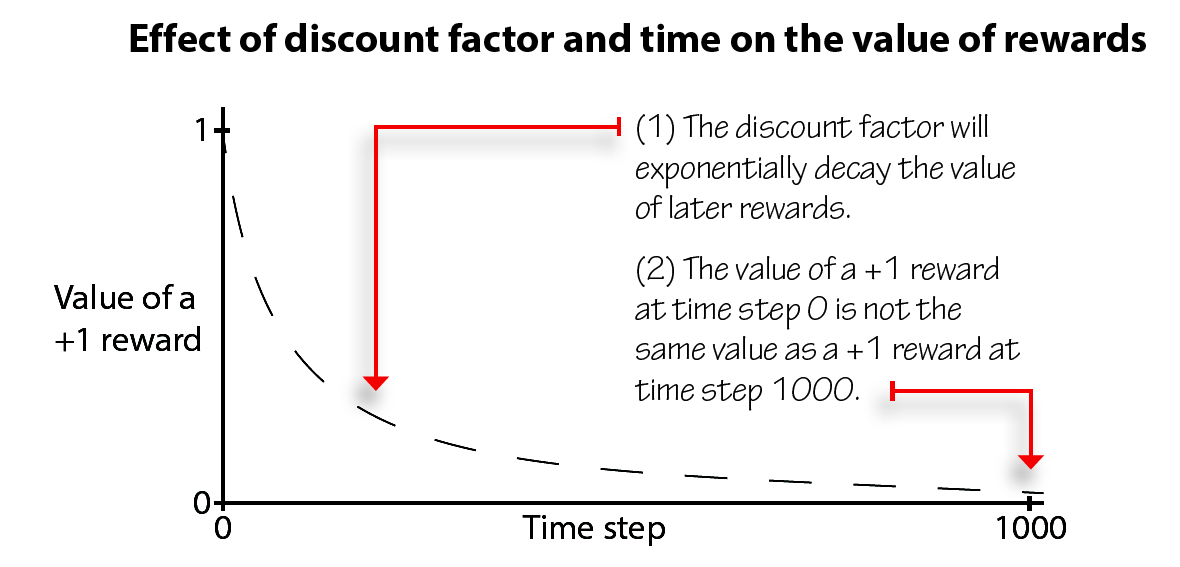
\includegraphics[scale=0.3]{captures/descuento.png}
	\caption{Ilustración gráfica del factor de descuento sobre la recompensas. Extraído de origen. \cite{book:miguel}}
	\label{fig:descuento} % Unique label used for referencing the figure in-text
	%\addcontentsline{toc}{figure}{Figure \ref{fig:GDS}} % Uncomment to add the figure to the table of contents
\end{figure}

Matemáticamente, la \textbf{recompensa acumulada} quedaría de la siguiente forma incluyendo el descuento:

\begin{equation*}
G_t=R_{t+1}+\gamma R_{t+2}+ \gamma^2R_{t+3}+...+\gamma^{T-1}R_T
\end{equation*}

Podemos simplificar esta ecuación y tener una más general:

\begin{equation*}
G_t=\sum^T_{k=0}\gamma^kR_{t+k+1}
\end{equation*}

Estos son los componentes y conceptos del los MDPs. Existe muchas extensiones y variables que se han desarrollado para adaptarlo de una manera más fiel y ajustada a un conjunto de problemas con características concretas. Por ejemplo, para problemas con observaciones parciales del entorno(POMDP), para problemas con acciones, estados y recompensas de valores continuos... No es objetivo de este proyecto ver todas las posibles variantes que la comunidad científica ofrece sobre este aspecto.

%\section{Experiencia}\label{sec:experiencia}
%
%La experiencia que se obtiene de un episodio puede ser extraída o analizada de distintas formas. Principalmente, un agente debe decidir una acción de las posibles a realizar en el entorno en el que se encuentra, pasando a un estado nuevo tras realizarla. Por tanto, estas acciones también producirán cambios en el entorno que a su vez cambiarán los datos que percibe el agente de dicho entorno. Se necesita un \textit{feedback} o retroalimentación que indique como de cerca esta su objetivo. Entonces, debemos de ser capaces de calcular una \textbf{recompensa} del entorno en cada momento para tener una orientación y que el agente sepa estimar cuando una acción es positiva o negativa para alcanzar su objetivo. \\
%
%La recompensa una vez alcanza un estado terminal está clara; positiva si ha logrado su objetivo, negativa si no lo ha conseguido. Sin embargo, no solo es conveniente saber cuando el agente consigue su objetivo o no. Si definimos en el problema algún \textbf{sistema de estimación de recompensas} por acción realizada, podremos construir una experiencia mucho más rica en el agente. Podríamos sacar información positiva o negativa de las decisiones tomadas en el transcurso de un episodio y no solo quedarnos con el desenlace del mismo. Es decir, todos los fracasos pueden tener acciones buenas y todos los aciertos pueden tener acciones malas. Si la detectamos, podemos aprender de una forma más eficiente y diversa, esa es la idea. \\
%
%Hay muchas formas de estimar esa recompensa, hay que tener en cuenta que en problemas como el juego de GO, una acción puede no ser útil hasta 100 jugadas más adelante o, por el contrario, pasarnos factura en esas 100 jugadas a futuro. \\
%
%Uno de los planteamientos más utilizados es la idea de \textbf{particionamiento} de la recompensa final del episodio durante todas las acciones o pasos del agente. ¿Cómo podemos particionar correctamente estas recompensas sin saber si esas influyen en el futuro como he mencionado antes? Una de las formas generales de hacerlo y que funcionan bastante bien en cualquier problema que pueda tener este tipo de dependencias a lo largo del tiempo es el \textbf{discounting}. \\
%
%Esta técnica hace que la recompensa de una jugada dependa, no solo del estado actual que deja el entorno, sino de la suma de recompensas anteriores que se obtuvieron ponderadas. se ponderan más las inmediatas a la actual y a medida que se encuentran más alejadas en términos de tiempo o número de acciones pasadas se va descontando esta ponderación para que su influencias sean menos significativas. \\
%
%\subsection{Representación de la experiencia}\label{sec:representacionexperiencia}
%
%La experiencia, visto de una forma más cercana a la programación, se suele almacenar en vectores o datasets. Por cada paso que el agente decide, se almacenan estos tres datos: \\
%
%\begin{itemize}
%	\item Observaciones del entorno(\textit{input}). \\
%	
%	\item Acción realizada(\textit{output}). \\
%	
%	\item Recompensa obtenida(\textit{reward}). \\
%\end{itemize}
%
%
%
%De esta manera el contenedor de experiencia irá aumentando a medida que avanza el episodio. Estos contenedores y la metodología que siguen para crearse cuando se ejecuta un agente tratan de ser \textbf{independientes} del problema que están resolviendo. En otras palabras, este sistema funciona igual independientemente del entorno o problema que se resuelve. Todos esos problemas tendrán su propia definición de inputs, outputs y recompensas y podrán ser utilizados en el momento que se decida entrenar y reforzar al agente con esa información adquirida. 

\section{Política}\label{sec:politica}

Ya hemos definido MDPs el cual es un motor y una arquitectura con su definición de componentes para representar los problemas de RL. En esta sección, pasamos de hablar de cómo \textbf{definir} un problema a cómo \textbf{solventar} un problema en MDPs. En términos generales, se necesita un \textbf{sistema} capaz de realizar una \textbf{secuencia de acciones} que trate de conseguir la mejor recompensa acumulada posible. Esto es lo que se conoce como \textbf{política} y es denotada como $\pi$.\\

Se trata de una función que devuelve una acción dado un estado del entorno. Una política puede ser cualquier función, no tiene por qué ser necesariamente ``inteligente''. Por ejemplo, una función \textbf{aleatoria} puede usarse como política, generalmente mala, pero una política al fin y al cabo. En un lado opuesto, una política puede ser una \textbf{red neuronal}(DRL), algo mucho más complejo que una función aleatoria.\\

Al igual que los propios problemas de MDPs, las políticas pueden ser tanto \textbf{estocásticas} como \textbf{deterministas}. Dada una observación $s$, en las políticas estocásticas tendremos como salida con distribución de probabilidades de todas las salidas(acciones) posibles, mientras que en una política determinista tendremos una única salida. \\

A continuación, veremos una serie de funciones que, junto con la política, nos permite describir, evaluar y mejorar el comportamiento de la misma, estas son:\\

\begin{itemize}
	\item Función de \textit{estado-valor}\\
	
	\item Función de \textit{acción-valor}\\
	
	\item Función de \textit{acción-ventaja}\\
\end{itemize}

\subsection{Función de estado-valor}

Uno de los principales requisitos que hay que conseguir es una forma fiable de \textbf{comparar} las políticas. Decidir entre varias cual es mejor para resolver un problema complejo no es algo sencillo. Para este cometido, se utiliza una función llamada \textbf{función de estado-valor}: 

\begin{equation*}
\upsilon_\pi(s)=\E\pi[G_t|S_t=s]
\end{equation*}

Esta función calcula una \textbf{previsión} de la recompensa acumulada a partir de un estado($s$) bajo una política concreta($\pi$). En otras palabras, estima como de bien se va a comportar una política a partir de un estado del entorno.\\

Si detallamos la función anterior, definiendo de una forma más específica la recompensa acumulada, tenemos lo siguiente:

\begin{equation*}
\upsilon_\pi(s)=\E\pi\left[\sum^\infty_{k=0}\gamma^kR_{t+k+1} | S_t=s\right]
\end{equation*}

Teniendo esta función podemos comparar políticas diferentes para un mismo problema, partiendo de un idéntico estado para ambas:

\begin{equation*}
\pi\geq\pi'\iff\upsilon_\pi(s)\geq\upsilon_{\pi'}(s) 
\end{equation*}

Se asume que existe una política óptima ($\pi_*$), lo cual quiere decir que no existe otra política mejor que esa y el objetivo es aproximar una política lo máximo posible a ésta:

\begin{equation*}
\pi_* \geq \pi' \forall \pi'
\end{equation*}

\subsection{Función de acción-valor}

En lugar de comparar una previsión de recompensas acumuladas a partir de un mismo estado para dos políticas diferentes, esta \textbf{función de acción-valor} trata de valorar la realización de una acción $a$ en un estado $s$. Si tenemos una buena función que determine esto, podría ser de gran utilidad a la hora de decidir entre acciones y de esta manera \textbf{mejorar} las políticas. \\

Entonces, trata de estimar la recompensa acumulada de una política $\pi$ después de haber realizado una acción $a$ en un estado $s$:

\begin{align*}
q_\pi(s,a)&=\E\pi\left[G_t|S_t=s,A_t=a\right]\\
q_\pi(s,a)&=\E\pi\left[\sum^\infty_{k=0}\gamma^kR_{t+k+1}|S_t=s,A_t=a\right]
\end{align*}

Vemos que la nomenclatura es muy similar a la función \textit{estado-valor}, dado que el objetivo es el mismo solo que teniendo en cuenta una acción en ese estado antes de calcular esa recompensa acumulada. Esto puede ayudar a considerar el \textbf{dinamismo} del entorno y como cambia la expectativa de recompensa final acumulada obtenida a partir de las acciones que se realizan.

\subsection{Ecuación de Bellman}\label{sec:bellman}

La función de \textit{estado-valor} puede ser expresada \textbf{recursivamente}. Esto es conocido como \textbf{Ecuación de Bellman}:

\begin{align*}
\upsilon_\pi(s)&=\E\pi\left[G_t|S_t=s\right] \\
&= \E\pi\left[R_{t+1}+\gamma G_{t+1}|S_t=s\right]\\
&= \E\pi\left[R_{t+1}+\gamma \upsilon_\pi(S_{t+1})|S_t=s\right]
\end{align*} 

Partimos de lo aprendido hasta el momento; la recompensa acumulada es la suma de la recompensas hasta el fin del episodio, junto con la ponderación del valor de descuento exponencial($\gamma$). Si expresamos la acumulación de recompensa como la primera recompensa obtenida más la acumulación de recompensas siguientes multiplicadas por gamma(elevado a 1 por calcularse a partir del estado siguiente), podemos volver a obtener una función \textit{estado-valor} y, por tanto, una función \textbf{recursiva}.\\

Esto resulta bastante interesante, ya que nos percatamos de que el valor de un estado depende recursivamente de los valores posibles de otros muchos estados futuros, incluyendo los estados originales a los que se llegará en el momento de llevarlo a la práctica. \\

Los algoritmos pueden iterar en esta ecuación y resolver el valor de estado para un entorno completo. A su vez, se puede extraer una conclusión a partir de este concepto. En una idílica política óptima, la función \textit{estado-valor} siempre será igual a la función de \textit{acción-valor} para la acción $a$ que estime el mejor valor en $s$ (la mejor acción posible), ya que partimos del supuesto de que siempre elige la mejor acción al ser la mejor política:

\begin{align*}
&\upsilon_{\pi_*}(s) = max(q_{\pi_*}(s,a))\\
&a \in A(s)
\end{align*}

Recordemos que $A(s)$ hace referencia al conjunto de acciones posibles en el estado $s$. 


\subsection{Función de acción-ventaja}\label{sec:ventaja}

Esta es una función que se deriva de las dos anteriores. También conocida como \textbf{función de ventaja}, es la diferencia de recompensas acumuladas estimadas por la función \textit{acción-valor} de una acción $a$ en un estado $s$ y la función \textit{estado-valor} del estado $s$ bajo la política $\pi$:

\begin{equation*}
a_\pi(s,a)=q_\pi(s,a)-\upsilon_\pi(s)
\end{equation*}

Esta función determina como de bueno es coger la acción $a$ en lugar de seguir la política $\pi$.

%Hablar de que la ventaja puede ser utilizada como medidor de relevancia en un episodio? 

\subsection{Evaluando una política}\label{sec:evaluacion}

Utilizando estas funciones podemos evaluar el nivel de bondad de una política cualquiera definida en un problema MDPs. Ya se mencionó que utilizando la función \textit{estado-valor} era posible decidir cuando una política es mejor que otra. \\

Explicamos la nomenclatura y el concepto de esta función. Ahora vamos a explicar una de las técnicas utilizadas para definirla dado un problema MDPs y una política que resuelve dicho problema.

Este algoritmo es conocido como \textbf{Evaluación iterativa de política}. Consiste en calcular la función \textit{estado-valor} de una política recorriendo el espacio de estados($S$) y mejorando dichas estimaciones de forma \textbf{iterativa}:

\begin{equation*}
\upsilon_{k+1}(s)=\sum_a\pi(a|s) \sum_{s',r}p(s',r|s,a)\left[r+\gamma\upsilon_k(s')\right]
\end{equation*}

La variable $k$ hace referencia a la iteración que está ejecutando. Vayamos por partes, $\upsilon_0(s)$ será la asignación inicial de estimaciones por parte de la función \textit{estado-valor} para cada estado $s \in S$ con la política que estamos evaluando, serán valores arbitrarios y 0 en caso de que el estado sea terminal para cada estado $s \in S$. \\

$\pi(a|s)$ hace referencia a la probabilidad de ejecutar una acción $a$ en el estado $s$ por parte de la política. Para simplificar, asumamos una política determinística, por lo que el valor será directamente 1. \\

$s'$ y $r$ hacen referencia al siguiente estado y recompensa obtenida tras realizar dicha acción por parte de la política. Como ya se ha mencionado anteriormente, una acción $a$ puede desencadenar más de una $s'$ diferente, dependiendo de si el problema es estocástico o no, por eso se habla de probabilidad de $s'$ y $r$ sabiendo el estado $s$ y acción $a$ realizada. \\

Esta segunda parte calcula el valor del estado $s$ como la suma ponderada de la recompensa  y el valor estimado para el siguiente estado $s'$ con su correspondiente descuento en caso de tenerlo. \\

Esta función la podemos ejecutar iterativamente de tal forma que estaremos aproximando el valor de $\upsilon_\pi(s)$ a su valor real para cada estado del problema. Este valor converge en el \textbf{infinito}. En la práctica, deberemos establecer un \textbf{umbral}($\theta$) en el que si el valor nuevo no tiene una diferencia absoluta mayor que $\theta$, se considere por aproximado correctamente y finalice. \\

Al tenerse en cuenta ese factor de \textbf{aleatoriedad} en reacciones del entorno ante las acciones, el valor que vamos a ir convergiendo para cada estado será la recompensa acumulada esperada que obtendremos si ejecutamos muchos episodios con esa política desde ese estado. En la realidad no se obtiene esa recompensa de manera exacta a partir de ese estado y esa política. No olvidemos que estamos hablando de \textbf{estimaciones}. \\

Nos damos cuenta que en el momento que hagamos más de una iteración, estaremos estimando recompensas a partir de estimaciones de recompensas. Esto es conocido como \textbf{bootstrapping} y es muy utilizado como técnica dentro de RL y DRL.

\subsection{Mejorando una política}

El siguiente paso es utilizar estos valores de evaluación de políticas a nuestro favor para poder \textbf{mejorarlas}. El ejemplo más sencillo de como hacerlo y menos eficaz sería generar muchas políticas aleatorias, evaluarlas e ir quedándonos con la mejor. \\

Lamentablemente, los problemas que se resuelven con estas técnicas suelen ser demasiado complejos como para alcanzar patrones y abstracción de conocimiento de una política de forma aleatoria. \\

Existen formas mucho más elegantes y mejores para inducir una mejora más eficiente. Vamos a hablar de la utilización de la función \textit{acción-valor} para conseguir este objetivo. \\

Con esta función obtendremos las estimaciones de recompensas para cada acción $a$ posible en cada estado $s$ del entorno. Entonces, podemos utilizar esa información para establecer una \textbf{guía} en la modificación de la política. \\

Si en el caso anterior calculábamos la función \textit{estado-valor} a partir de un algoritmo iterativo, veremos como calcular la función \textit{acción-valor} a partir de la primera y MDP, denominado \textbf{algoritmo de mejora de política}:

\begin{equation*}
\pi'(s)=argmax_a\sum_{s',r}p(s',r|s,a)\left[r+\gamma\upsilon_\pi(s')\right]
\end{equation*}

Recordemos que $\gamma$ es la tasa de descuento comprendida entre 1 y 0 y que $s'$ hace referencia al estado siguiente de $s$ tras realizar la acción $a$. Básicamente consiste en buscar aquellas acciones que nos lleven a estados siguientes con la estimación de \textit{estado-valor} más alta existente. \\

Cogiendo estas acciones que nos llevan a estados con estimaciones \textit{estado-valor} más alto en lugar de la acción por la que optaría la política $\pi$ en sí misma, estamos creando una nueva política denotada como $\pi'$, la cual vemos que sigue una estrategia \textbf{voraz} o greedy, dado que siempre sigue el mismo patrón en la selección de la siguiente acción. \\

Recordemos también que la función \textit{estado-valor} calcula una estimación sumando todas las recompensas estimadas de todos los siguientes estados posibles (ecuación de Bellman en el que se explica esta recursividad), esto es lo que se utiliza para cada acción en un estado concreto y nos quedamos con el máximo existente. Como consecuencia directa, esta función también es una aproximación que tratamos que sea lo más leal a la realidad posible. \\

A partir de este concepto, nos percatamos de que existe un \textbf{ciclo} que podemos repetir mientras que la política siga mejorando: \\

\begin{enumerate}
	\item Calculamos la función \textit{estado-valor} con el \textbf{algoritmo iterativo de evaluación} para una política $pi$ en un problema MDP. \\
	
	\item Calculamos la función \textit{acción-valor} con el \textbf{algoritmo de mejora de política} el cual parte de la función de \textit{estado-valor} previamente calculada. \\
	
	\item Utilizando la función \textit{acción-valor}, podemos generar una nueva política. \\
	
	\item Recalculamos la función \textit{estado-valor} de esta nueva política y repetimos el proceso siempre que haya un cambio significativo positivo en las estimaciones de la misma(mayor que $\theta$). \\	
\end{enumerate}

Llegará un momento en el que la política converge y no se obtiene nada nuevo y mejor utilizando este proceso.

\section{Exploración vs Explotación}\label{sec:probabilidades}

Todo lo explicado hasta ahora referente a la evaluación y mejora de las políticas funciona muy bien cuando sabemos de antemano como va a reaccionar el entorno a cada una de las acciones que se realizan en el mismo por parte del agente. \\

\textbf{Sabiendo} exactamente la \textbf{función de transición} y la \textbf{función de recompensa} del problema MDP podemos obtener una \textbf{política óptima} sin la necesidad de que el agente interactúe con el entorno, dado que podemos estudiar las posibilidades que ofrece el problema de forma directa. Por desgracia, la mayoría de problemas planteados no son tan predecibles, ni podemos asumir la \textbf{propiedad de Markov} para simplificar la transiciones de los entornos. \\

Sabiendo lo que sabemos llegados a este punto, ahora es necesario buscar una manera de que el agente pueda aprender mientras lidia con la \textbf{incertidumbre} en las transiciones de estados del entorno. Es lo que se conoce como \textbf{aprendizaje de ensayo y error}. \\

Esto plantea una serie de inconvenientes nuevos a la hora de mejorar la política del agente. Hay que decidir, dado un entorno $s$, si \textbf{explota} su propio conocimiento estimando las recompensas como hemos visto hasta ahora para obtener su mejor acción $a$ para esa política $\pi$ o si, como medida alternativa, decide \textbf{explorar} nuevos posibles desenlaces del entorno realizando acciones no óptimas bajo su política actual para generar nuevas interacciones sobre las que aprender. \\

Al no tener una función de transición perfectamente definida, se añade el problema de no saber si las estimaciones que tenemos sobre el valor de los estados y acciones son suficientemente buenas. \\

La respuesta es el \textbf{equilibrio}. La exploración va a permitir obtener un conocimiento que va a permitirnos ser más efectivos en las estimaciones de valores y, por tanto, en la explotación de la política. \\

Existen varias forma de introducir exploración en los problemas:

\begin{itemize}
	\item \textbf{Estrategias de exploración aleatoria}: Es el más popular. El agente explota su política la mayoría de veces, y en algunas ocasiones explora utilizando una acción aleatoria. Es conocido como \textit{$\epsilon$-Greedy}, siendo $\epsilon$ un valor muy pequeño que representa la probabilidad de explorar en lugar de explotar.\\
	
	\item \textbf{Estrategias de exploración optimistas}: Es más sistemático que el anterior. Incrementa la preferencia de estados en los que hay un mayor factor de incertidumbre(son desconocidos por parte del agente), pudiendo provocar que el agente realice acciones con mayor probabilidad de transitar a estos estados en lugar de utilizar la acción óptima para su política dada.\\
	
	\item \textbf{Estrategias de exploración de información de espacio de estado}: Trata de enriquecer la información aportada por los estados del entorno, codificando un grado de incertidumbre como parte de dichos estados. Es una forma de diferenciar por parte del agente qué estados han sido explorados y cuales no.\\
\end{itemize}

Existe una gran cantidad de opciones a la hora de administrar la explotación y exploración en un agente, incluso variantes de las explicadas. Es uno de los principales retos a resolver por parte de RL.

%Es esencial que el agente \textbf{experimente} con la finalidad de que aprenda de situaciones en las que, por como funciona, nunca se vería implicado debido a las decisiones que está habituado a tomar y que sabe que normalmente funcionan. \\

%Algunas de las soluciones para darle esa \textbf{exploración} en su árbol de decisiones puede ser que tome decisiones aleatorias en el 1\% de las ocasiones, por ejemplo. Otra sería idear este \textbf{muestreo de distribución de probabilidad} de tal manera que cada acción tuviera un porcentaje de probabilidad de que el agente la ejecutara. Por tanto, esto haría que no siempre se seccionase la acción más apoyada por el agente. Sería una forma de introducir esa \textbf{aleatoriedad dirigida} al mismo tiempo que no se desestima el \textbf{criterio actual} que tiene. \\

%Entonces, hay que procurar que el agente no sea muy \textbf{estricto} en el calculo de estas distribuciones, ya que si una acción determinada adquiere el valor 1 y el resto de acciones el valor 0, no valdrá de nada la idea que acabamos de explicar. Esto puede ser un problema muy frecuente sobretodo en los primeros compases de aprendizaje con estas técnicas, por lo que debemos tener cuidado con esto.

\section{Aprendiendo a evaluar y mejorar políticas}

En el apartado \ref{sec:evaluacion} vimos la \textit{Evaluación iterativa de política}, la cual nos permitía evaluar un problema MDP de forma matemáticamente directa sin la necesidad de que el agente tuviera que interactuar con el entorno previamente para optimizar sus funciones valor. \\

Vuelvo a insistir, uno de los principales desafíos del RL reside en que los agentes en la gran mayoría de problemas no pueden ver el MDP subyacente que rige el problema y el entorno. Más concretamente, las funciones de transición y de recompensa son \textbf{ruidosas}, lo cual hace al entorno mucho más hostil y que no pueda ser evaluado de forma directa, a no ser que exploremos sobre el mismo. A esto se le llama \textbf{problema de predicción}. \\

Cuánto mejor seamos capaces de \textbf{estimar} las recompensas futuras, a pesar de la incertidumbre de estos problemas, mejor capacidad tendremos para \textbf{mejorar} nuestro agente por medio del feedback que recibe de su propio desempeño con el entorno(\textbf{aprendizaje de ensayo-error}). \\

Entonces, a modo de condensación de conceptos, vamos a hacer hincapié en los siguientes: \\

\begin{itemize}
	\item \textbf{Recompensa($r$)}: Es el valor que devuelve el entorno después de realizar una acción sobre él mismo, viene dado por su función de recompensa definida. Es uno de los datos más relevantes del RL, pero no es el valor que tratamos de maximizar, ya que no permite aprender conocimientos y estrategias con buenos planteamientos a medio o largo plazo por parte del agente. \\
	
	\item \textbf{Recompensa acumulada($G_t$)}: Finalizado un episodio, es la suma de recompensas que se han ido produciendo en cada uno de sus \textit{time-steps}. Si tiene un sistema de descuento con $\gamma$ las recompensas irán perdiendo relevancia a medida que el episodio se prolonga más. Este dato es más representativo para el conocimiento que estamos tratando de conseguir, ya que tiene en cuenta la secuencia de acciones completas y estrategias a largo plazo. No obstante, de nuevo, no es el valor que estamos tratando de optimizar para el agente. Un agente que trate de obtener la recompensa acumulada más alta posible puede desarrollar una política con comportamientos ruidosos (si el episodio se prolonga en el tiempo puede obtener recompensas más altas). Es posible que se consiga una política con muy buen rendimiento, pero lo más probable es que no sea así.\\
	
	\item \textbf{Función de valor}: Hace referencia a la \textbf{estimación} de recompensa acumulada que se obtiene de antemano. Por lo que es un valor que se consigue durante cada \textit{time-step} del episodio y no necesitamos que finalice para conocerlo.\\
\end{itemize}

Éste último es el valor que tratamos de \textbf{optimizar}. Al ser la mayoría de problemas estocásticos y no saber con certeza las transiciones de estados del entorno, tener unas medias altas de estimaciones para una acción dada ayuda a \textbf{generalizar} ese conocimiento a pesar del propio ruido del entorno.

\subsection{Método de Montecarlo}

El objetivo final, como bien sabemos, es conocer el valor de una política; cómo de buena es. Dicho de otra forma, el objetivo es estimar la función \textit{estado-valor} $\upsilon_\pi(s)$ de la política $\pi$ lo mejor posible. \\

El \textbf{Método de Montecarlo} consiste, en términos generales, en ejecutar un número considerable de episodios con la política a evaluar de tal manera que se almacenan cientos de trayectorias posibles de estados y acciones. Después se calcularía el \textbf{promedio} de recompensas acumuladas para cada estado. \\

La principal ventaja de este método es la sencillez de su implementación. Una vez finaliza un episodio, se almacena cada estado, acción, recompensa y estado siguiente obtenido como una \textbf{tupla de experiencia}. Cuando juntamos todas las tuplas de experiencia de un episodio(desde su estado inicial hasta el terminal), tenemos lo que se denomina como una \textbf{trayectoria}. \\

\begin{figure}[H]
	\centering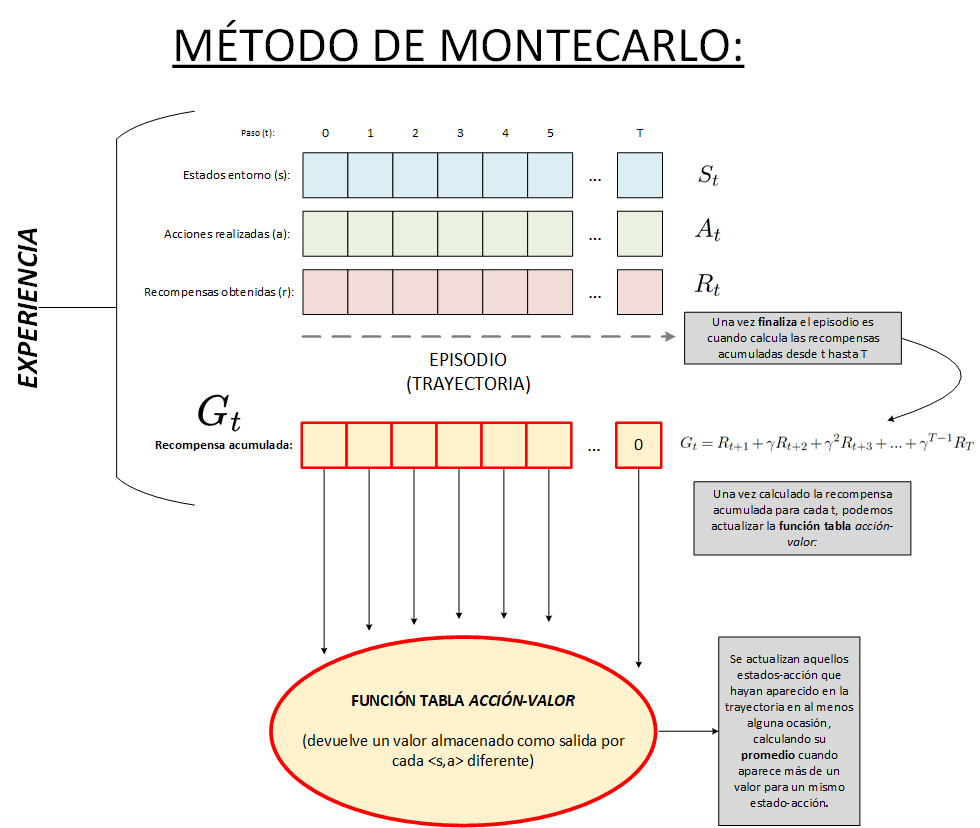
\includegraphics[scale=0.8]{captures/montecarlo.png}
	\caption{Esquema Método Montecarlo. Tabla función extraída de origen. \cite{article:RLromero}}
	\label{fig:montecarlo} % Unique label used for referencing the figure in-text
	%\addcontentsline{toc}{figure}{Figure \ref{fig:GDS}} % Uncomment to add the figure to the table of contents
\end{figure}

Una vez se obtiene una trayectoria, calculamos el valor de \textbf{recompensa acumulada} que hubo desde cada estado hasta su estado final o, lo que es lo mismo, finalización del episodio, aplicando descuentos de forma exponencial como hemos hecho siempre. Entonces, tendremos una recompensa acumulada diferente por cada uno de los \textit{time-steps} del episodio. Este valor se denota como $G_{t:T}$ siendo $t$ el \textit{time-step} actual y $T$ el último \textit{time-step} del episodio. \\

Ya se ha terminado de formar la trayectoria. El siguiente paso es estimar la función \textit{estado-valor} simplemente calculando el promedio de recompensa acumulada obtenida en cada estado de la trayectoria, ya que un estado puede repetirse en más de una ocasión dado un episodio. Entonces, la función simplemente consiste en almacenar un valor promedio por cada estado diferente del entorno, se trata de una \textbf{función tabla} tal y como podemos observar en la figura \ref{fig:montecarlo}.\\

También se puede realizar este método para calcular la función \textit{acción-valor} ($q_\pi(s,a)$). La forma de hacerlo es igual, solo que para los promedios se tendría en cuenta los estados y acciones juntos $<a,s>$. Dicho de otra forma, se diferenciaría entre dos estados iguales en los que se realizó acciones diferentes. Cada actualización de la función valor nos permite modificar la política y tratar de mejorarla, como ya se ha explicado en otras ocasiones.

\begin{verbatim}
for i = {0, ..., n_episodios}
    Calcular trayectoria del episodio
    Actualizar la función estado-valor o acción-valor
    Obtener política mejorada a partir de esta nueva función
\end{verbatim}

¿Cómo se calcula ese promedio una vez tenemos formada una trayectoria completa? Se puede hacer de dos maneras, y ambas son demostradas y aceptadas como buenas: \\

\begin{enumerate}
	\item Tomar la \textbf{media} de los valores G para cada estado $<s>$ o estado-acción $<s,a>$ dependiendo de si estamos hablando de $\upsilon_\pi(s)$ o de $q_\pi(s,a)$ respectivamente. \\
	
	\item En lugar de calcular la media, quedarse con el \textbf{primer valor G} encontrado para cada estado o estado-acción, de nuevo dependiendo de la función que estemos calculando. \\
\end{enumerate}

Como ya mencionamos en el apartado \ref{sec:probabilidades}, la exploración es muy importante para los problemas de RL. Por ello, en lugar de la política $\pi$ podemos utilizar la variante \textit{$\epsilon$-greedy}. Con probabilidad $\epsilon$ generamos una acción aleatoria y la acción respondida por $\pi$ en caso contrario. \\

El principal requisito que debemos tener en cuenta, directamente deducible de el funcionamiento de este método, es que solo podemos actualizar la función valor cuando el agente \textbf{finaliza} cada episodio, y no durante. Aunque existe una forma de poder actualizarse y mejorar paso a paso en su lugar.

\subsection{Métodos de Diferencia Temporal(SARSA)}

La principal desventaja del método de Montecarlo reside en su baja precisión en los problemas que superan una cierta complejidad de estados y acciones con alta incertidumbre de la transiciones de los mismos.\\

Esto se debe a que $G_{t:T}$; la recompensa acumulada desde el punto en el que se estudia hasta el final del episodio con el que se está aprendiendo, suele tener mucha varianza debido a este problema. Es decir, El \textbf{ruido} del propio problema hace que un estado o estado-acción en una trayectoria tenga una recompensa acumulada muy distinta en otra trayectoria futura que genere. \\

La forma de combatir este ruido para Montercarlo son los datos, recolectar toda la experiencia y trayectorias que pueda, para tratar de obtener mejores promedios y compensar de alguna manera el ruido. \\

El \textbf{Método de Diferencia Temporal}(SARSA) propone sustituir $G_{t:T}$ por la suma de la recompensa actual que recibe el agente del entorno $R_{t+1}$ tras realizar su acción $A_t$ con la estimación de función valor que es capaz de realizar con su política actual $\pi$ y ponderada con el factor de descuento $\gamma$, ya que se trata de una interacción siguiente a la que estamos estudiando. De nuevo, se puede utilizar tanto para calcular la función \textit{estado-valor}, utilizada para evaluar políticas, como su función \textit{acción-valor}, utilizada generalmente para mejorar dichas políticas:

\begin{align*}
\upsilon_\pi(S_t) &\leftarrow \upsilon_\pi(S_t)+\alpha\left[R_{t+1}+\gamma \upsilon_\pi(S_{t+1}) - \upsilon_\pi(S_t)\right] \\
q_\pi(S_t,A_t) &\leftarrow q_\pi(S_t,A_t)+\alpha\left[R_{t+1}+\gamma q_\pi(S_{t+1},A_{t+1}) - q_\pi(S_t,A_t)\right]
\end{align*}

El valor $\alpha$ se usa para ponderar el \textbf{cambio} de la función valor. En cada paso de entrenamiento si $\alpha=1$ no se tiene en cuenta el valor previo de la función. Si $\alpha=0$, se mantiene el valor previo y no experimenta una actualización de la función en ese paso.\\

Ese \textbf{cambio} del que estamos hablando consiste en sumarle a la función actual la diferencia de ella misma con el nuevo sistema en el que se tiene en cuenta la recompensa actual y estimación a partir del estado siguiente $s'$ con esa función.\\

Podemos ir calculando las nuevas funciones valor durante cada \textit{time-step} y recompensa que obtiene sin tener que esperar a que finalice un episodio, aunque no es la única ventaja. \\

La principal consecuencia de este hecho y diferencia entre SARSA y MonteCarlo es que conseguimos tener una \textbf{varianza} mucho menor. Esto ocurre porque SARSA depende solo de una acción y recompensa que se obtiene en ese mismo instante, el resto del valor es estimado con su función valor actual. \\

Estas estimaciones, dependiendo en el estado de desarrollo que se encuentren, van considerando cada vez mejor el ruido del problema que está tratando de solventar. Cosa que no ocurre con $G_{t:T}$, ya que es específico de la trayectoria y experiencia con la que esté trabajando en ese momento. \\

La conclusión final es que los métodos de diferencia temporal convergen más rápido que Montecarlo en términos generales. \\ 

\begin{figure}[H]
	\centering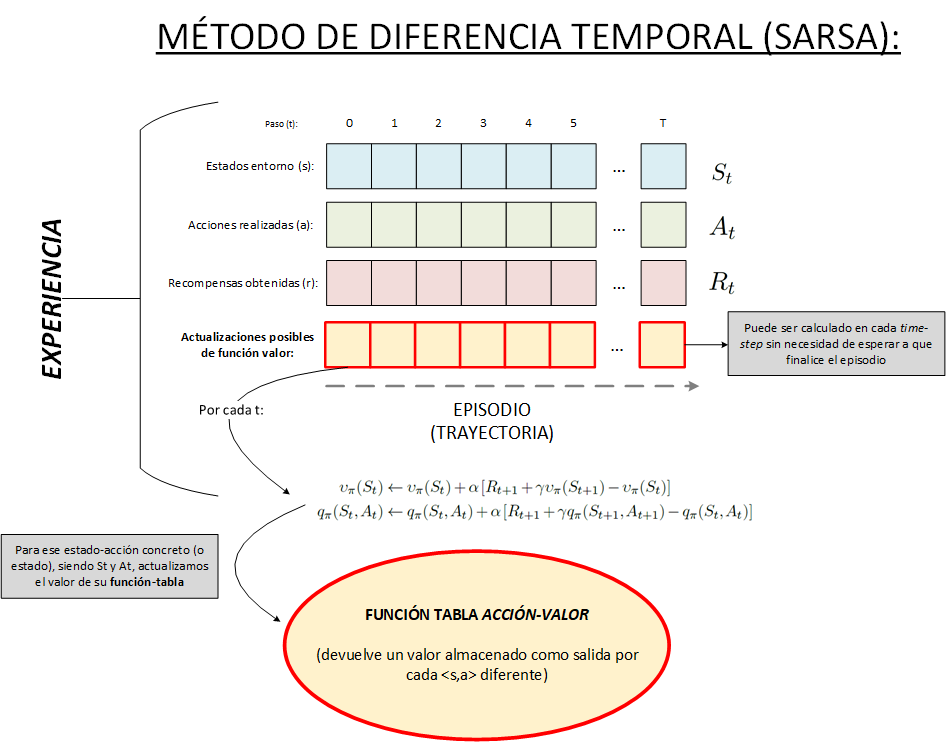
\includegraphics[scale=0.8]{captures/SARSA.png}
	\caption{Esquema Método de diferencia temporal(SARSA). Tabla función extraída de origen. \cite{article:RLromero}}
	\label{fig:SARSA} % Unique label used for referencing the figure in-text
	%\addcontentsline{toc}{figure}{Figure \ref{fig:GDS}} % Uncomment to add the figure to the table of contents
\end{figure}

Calcular estimaciones a partir de estimaciones es un concepto que ya ha sido mencionado; estamos hablando de \textbf{bootstrapping}, muy común en el mundo de RL como podemos observar.\\

También es posible establecer \textbf{puntos intermedios} entre Montecarlo y SARSA. No se actualiza las funciones valor ni cuando finaliza un episodio, ni de forma inmediata cada vez que se produce un \textit{time-step}. En su lugar, actualizamos cada $n$ interacciones. Durante esas $n$ interacciones utilizaremos la recompensa acumulada $G_{t:t+n}$, para el resto de acciones, hasta el supuesto final del episodio, volvemos a recurrir a las estimaciones de recompensas(bootstrapping):

\begin{align*}
&G_{t:t+n}+\upsilon_\pi(S_{t+n+1}) \\
&G_{t:t+n}+q_\pi(S_{t+n+1},A_{t+n+1})
\end{align*}

No es objetivo de este trabajo entrar en mayor detalle con estos algoritmos debido a que es suficiente para entender su arquitectura y funcionalidad dentro de los problemas de RL.

\subsection{Q-Learning}\label{sec:qlearning}

Se trata de un modelo \textbf{libre de política} y con \textbf{bootstrapping}. Aproxima directamente la política óptima. Esto quiere decir que el agente puede actuar aleatoriamente y aún así encontrar la función valor y política óptima, veremos como es esto posible. Se trata de una propuesta diferente conceptualmente a las dos mostradas anteriormente, vamos a explicar cada parte con mayor detalle. \\

Si volvemos al ejemplo de SARSA, se trata de un modelo conocido como \textbf{On-Policy}, ya que depende de su propia política para poder mejorarse, por lo que es capaz de aprender de sus propios errores y aciertos. Esto las hace excelentes, sin embargo, esto hace al mismo tiempo que no sea capaz de aprender de ``los errores de otro'', cosa que hacemos los humanos constantemente. \\

Por ejemplo, si alguien que está delante de nosotros tropieza con una piedra, generalmente vamos a aprender a evitarla antes de experimentar un tropiezo. Los modelos \textbf{On-Policy} son muy buenos, pero no aprenden fuera de la experiencia que hayan generado ellos mismos, por cuestiones matemáticas obvias vistas en las fórmulas anteriores. \\

El aprendizaje \textbf{Off-Policy}, por otra parte, es capaz de hacerlo. Puede aprender de una política que es diferente de la política generadora de experiencia. A esto es a lo que nos referimos con \textbf{libre de política} para el Q-Learning. En este tipo de aprendizaje tenemos dos tipos de políticas funcionando:\\

\begin{itemize}
	\item \textbf{Política de comportamiento}: Utilizada para generar experiencia, interactuando con el entorno de forma directa.\\
	
	\item \textbf{Política objetivo}: Es la política sobre la que se realiza el aprendizaje y mejoras.\\
\end{itemize}

Durante las trayectorias de episodios con experiencia, tendremos en las estimaciones por \textit{time-step} lo siguiente:

\begin{align*}
Q_\pi(S_t,A_t) \leftarrow Q_\pi(S_t,A_t)+\alpha\left(R_{t+1}+\gamma max_{a\in A(S_t)}Q(S_{t+1},a) - Q(S_t,A_t)\right)
\end{align*}

Tenemos una función \textit{acción-valor} que denominaremos $Q(s,a)$. Para estimar las recompensas futuras en cada uno de los pasos de una trayectoria, hacemos una operación muy similar a SARSA, ya que también realiza un aprendizaje paso a paso y no episodio a episodio como Montecarlo. La principal diferencia viene dada en la \textbf{actualización} de la política. En SARSA, utilizábamos la diferencia de esa función con la suma de recompensa actual y estimación siguiente. En esta ocasión la estimación siguiente, es otra política que elige la mejor acción que considera Q (que es $a \in A(s)$), en lugar de elegir la acción con la que realmente se está produciendo esa experiencia (que es $A_t$).\\

\begin{figure}[H]
	\centering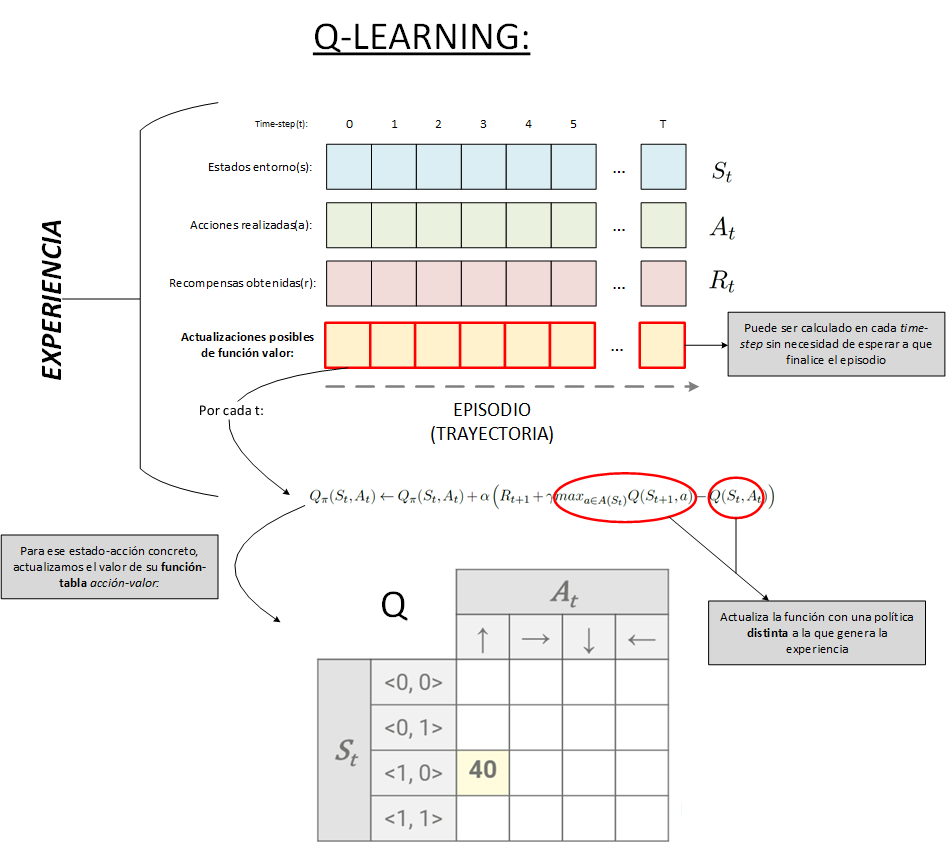
\includegraphics[scale=0.8]{captures/Q-Learning.png}
	\caption{Esquema Método Q-Learning. Tabla función extraída de origen. \cite{article:RLromero}}
	\label{fig:qlearning} % Unique label used for referencing the figure in-text
	%\addcontentsline{toc}{figure}{Figure \ref{fig:GDS}} % Uncomment to add the figure to the table of contents
\end{figure}

Para la exploración, podemos seguir utilizando $\epsilon$-greedy(Q) a la hora de realizar las estimaciones de recompensa con las acciones que tendría la política objetivo. \\

Existe algunas variantes como \textbf{Double Q-Learning}, la cual se basa en tener dos políticas objetivo en lugar de una. Es una estimación cruzada que ha mostrado mejores resultados en ciertas ocasiones, aunque no entraremos en más detalles con esta parte. \\

Como conclusión final, destacar la \textbf{independencia} de los problemas a resolver con las técnicas de RL vistas en estos apartados. Definiendo cada uno de los \textbf{componentes} del problema, como vimos en el apartado \ref{sec:componentesRL}, estas técnicas ya pueden entrenar agentes directamente, dado que tiene la forma de obtener experiencia y tratarla. Es una de las grandes ventajas de RL.

\chapter{Aprendizaje por Refuerzo Profundo(DRL)}

Hemos visto lo más importante y necesario de las técnicas de RL; su arquitectura y funcionamiento. Si recordamos el apartado \ref{sec:politica}, una política es una función que puede ser de cualquier forma, siendo una función totalmente aleatoria la más sencilla a la hora de devolver salidas ante el estímulo que ofrece el entorno del problema. \\

Con los métodos de Montecarlo, y sobretodo SARSA y Q-Learning (basado en SARSA), vimos formas más sofisticadas de utilizar el feedback del entorno para construir nuevas políticas a partir del aprendizaje por ensayo-error. Sin embargo, estos métodos simplemente guardaban un valor estimado por cada estado-acción diferente del entorno, en eso se basaban esas funciones valor de la política. \\

¿Y si en lugar de utilizar eso usamos como política redes neuronales? Si representamos las funciones como un conjunto grande de pesos y una red, estamos hablando del DRL. Las técnicas son muy parecidas a las explicadas hasta ahora, sin embargo, contamos con una nueva tecnología para estimar los valores de función que puede llegar a ser más potente. Sobretodo para abordar problemas complejos, no solo por su espacio de estados y acciones, sino por la cantidad de variables o información que puede tener cada uno de esos estados y acciones, sin contar que esta información puede ser continua y no discreta que directamente no puede ser recordada por una función tabla. \\

Vamos a ver algunas de las formas más importantes en las que se ha conseguido integrar el DL dentro del RL, para conseguir alcanzar estas ventajas respecto al RL original.

\section{Métodos Basados en Valor: Deep Q-Network(DQN)}\label{sec:DQN}

Es el primer algoritmo DRL que vamos a analizar. DQN es uno de los algoritmos más populares que hay dentro de este ámbito, siendo el inicio de una serie de investigaciones e innovaciones que marcaron un antes y un después en el mundo del RL. Con esta técnica fue la primera vez que se pudo crear un agente en ATARI capaz de resolverlo a partir de los píxeles crudos, de la propia imagen. Esto resulta muy interesante, las observaciones que el agente hacía del problema es exactamente igual a las que hace un humano, observar los píxeles de una imagen, en lugar de pensar anteriormente un formato de input específico para las observaciones del entorno. \\

Es una estrategia \textbf{basado en valor}(\textit{value-based}). Esta estrategia parte de la técnica de RL Q-Learning visto en el apartado \ref{sec:qlearning}, utilizando como funciones optimizables redes neuronales, vistas en el apartado \ref{sec:deeplearning}, lo que es comúnmente conocido como \textbf{Deep Q-Learning}.\\

El principal cambio reside en su función Q, modelándose como una \textbf{función no lineal}, lo cual permite trabajar con estados y acciones continuos como ya hemos comentado anteriormente. \\

Sabemos que para esta estrategia se tienen dos políticas diferentes; la generadora de experiencia y la objetivo. Sin embargo, esto no equivale a dos redes neuronales distintas. La arquitectura de la red neuronal como tal es la misma, lo que se cambia es el \textbf{conjunto de pesos} que define su comportamiento. Teniendo dos conjuntos de pesos diferentes, uno para cada cometido que hemos explicado. \\

Hay varias formas de plantear esa red neuronal. Si las acciones posibles del problema son discretas(no infinitas). Podemos crear una red neuronal que tenga tantas neuronas en la capa de entrada como variables una observación del estado $s$, y por otro lado, que la capa de salida tenga tantas neuronas(y por tanto,\textit{outputs}) como acciones posibles del problema. Representado cada una de esas salidas $Q(s,a;\theta) \forall a \in A$. \\

Para elegir una acción, podríamos coger la que tuviera un valor estimado más alto o aplicar una distribución de probabilidad para favorecer la exploración(esta decisión sería parte de la política $\pi$). Podemos observar dicha explicación en la figura \ref{fig:RNdiscreta}.

\begin{figure}[H]
	\centering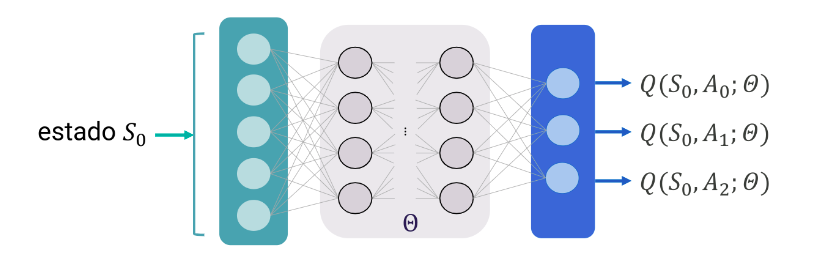
\includegraphics[scale=0.5]{captures/RNdiscreta.png}
	\caption{Esquema red neuronal, acciones discretas finitas. Imagen extraída de origen. \cite{article:RLromero}}
	\label{fig:RNdiscreta} % Unique label used for referencing the figure in-text
	%\addcontentsline{toc}{figure}{Figure \ref{fig:GDS}} % Uncomment to add the figure to the table of contents
\end{figure}

El símbolo $\Theta$ hace referencia al conjunto de pesos. \\

Por otra parte, podemos enfrentarnos a un problema que tenga acciones continuas y, por tanto, sean infinitas. La opción aquí sería incluir la acción como entrada de la red. Entonces, la salida sería $Q(s,a;\theta)$ para esa acción concreta. Si queremos $Q$ para otra acción, la parte de entrada de $s$ sería la misma y habría que modificar $a$. Al ser el número de acciones infinita, no podemos calcular todas las posibles acciones a partir de la entrada $s$ como en el caso anterior. Esto hace que DQN no sea apropiada para resolver este tipo de problemas, se puede adaptar \textbf{discretizando} el espacio de acciones, pero esto limita y simplifica en exceso la complejidad del problema. Lo vemos a continuación en la figura \ref{fig:RNcontinua}.

\begin{figure}[H]
	\centering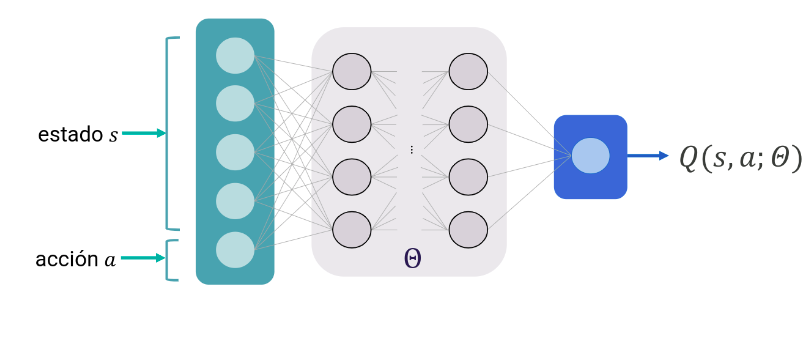
\includegraphics[scale=0.5]{captures/RNcontinua.png}
	\caption{Esquema red neuronal, acciones continuas infinitas. Imagen extraída de origen. \cite{article:RLromero}}
	\label{fig:RNcontinua} % Unique label used for referencing the figure in-text
	%\addcontentsline{toc}{figure}{Figure \ref{fig:GDS}} % Uncomment to add the figure to the table of contents
\end{figure}

Uno de los principales inconvenientes en las métodos basados en valor, es la \textbf{divergencia}, aunque hay propuestas científicas para prevenirla, no hay investigaciones sobre ello sólidas que permitan garantías totales. \\

En definitiva, el principal cambio entre Q-Learning y Deep Q-learning es la \textbf{sustitución} de la función-valor tabla por una red neuronal, con el potencial que esta nos ofrece frente a la anterior. ¿Pero como repercute dicho cambio en el proceso de entrenamiento? \\

Q-Learning permitía entrenarse paso a paso conforme experimentaba utilizando el \textit{método de diferencia temporal}(SARSA). No obstante, aquí se propone guardar una base de datos o también denominado \textbf{memoria de experiencias}. Esto hace que la experiencia pueda utilizarse en \textbf{cualquier orden} y \textbf{más de una vez}.\\

Esta adaptación trata de combatir dos problemas principales que tienen las estrategias basadas en valor(\textit{value-based}): en primer lugar, mejorar la \textbf{exploración} de dependencias entre zonas, ya que la experiencia se genera de forma secuencial. Por otra parte, con el método Q-Learning tradicional, no podíamos utilizar varias veces un paso o pasos de la experiencia que fuesen interesantes para el modelo. \\

Si recordamos el apartado \ref{sec:deeplearning}, las redes neuronales necesitan, entre otras cosas, una \textbf{función de error o pérdida} para posteriormente poder optimizar sus pesos con una \textbf{función de optimización} que se aproveche de esta información. \\

El problema es que no sabemos la respuesta óptima(o etiqueta original cuando hablábamos de aprendizaje supervisado). Es parte del paradigma del aprendizaje por refuerzo, existe tal incertidumbre y ruido en el entorno que es imposible en la mayoría de ocasiones saber la respuesta óptima, y la exploración (aprendizaje ensayo-error) es la única forma de poder acercarnos o aproximarnos a la mejor respuesta posible en cada una de las situaciones que nos plantea el entorno. \\

Una vez más, hay que \textbf{estimar} la respuesta óptima para poder tener una función de error para nuestra red neuronal, esto sería el entrenamiento del conjunto de pesos para nuestra política objetivo:

\begin{equation*}
Q(S_0,A_0) \leftarrow Q(S_0,A_0) + \alpha \left[R_1+\gamma max_{a\in A}Q(S_1,a)-Q(S_0,A_0)\right]
\end{equation*}

Con esa formulación podemos estimar la recompensa acumulada real que esperaríamos del entorno al final del episodio, a partir de un estado, acción , siguiente estado y recompensa, como ya hemos visto. \\

Cuanto mejor aproximemos Q, mejor será nuestra función de error para la red neuronal en sí. Por ejemplo, podríamos utilizar el error cuadrático(\textit{MSE}):

\begin{equation*}
MSE= \E\pi[(Q(S,A)-Q(S,A;\theta))^2]
\end{equation*}

Entonces, se debe producir una \textbf{actualización de los pesos} en la red ($\Delta\Theta$) denotada con la siguiente expresión

\begin{align*}
&\Delta\Theta = \Delta w = -\eta \mfrac{\delta E}{\delta w} \\
&\mfrac{\delta E}{\delta w} = 2(Q(S,A)-Q(S,A;\Theta))\mfrac{\delta Q(S,A;\Theta)}{\delta w}\\
&\mfrac{\delta Q(S,A;\Theta)}{\delta w}=\nabla_\Theta Q(S,A;\Theta) \\
&\Delta\Theta=-2\eta(Q(S,A)-Q(S,A;\Theta))\nabla_\Theta Q(S,A;\Theta) 
\end{align*}

Si simplificamos y aplicamos la expresión de Q-Learning que ya sabemos:

\begin{equation*}
\Delta\Theta=\alpha\left[R+\gamma max_{a \in A} Q(S',a;\Theta)\right]\nabla_\Theta Q(S,A;\Theta) 
\end{equation*}

Toda esta formulación matemática describe cómo se va a realizar esos cambios en los pesos que mencionamos a partir de cada tupla de experiencia. Vemos que se aplica el \textbf{gradiente de los pesos} para dicho cometido, parecido al que se mencionó en el apartado \ref{sec:optimizacion}, solo que la formulación es diferente por el hecho de combinarlo con Q-Learning.\\

Podemos aplicar una estrategia de \textit{mini-batches} (mini-lotes) extraido de la memoria de experiencias; esto quiere decir subconjuntos para realizar entrenamientos de los pesos.  \\

Estamos actualizando una aproximación a partir de una aproximación. Una vez más, aparece el ya conocido concepto de \textbf{bootstrapping}. Por ello, se utilizan dos redes $\Theta$, lo cual significa dos políticas diferentes, identificativo de la metodología Q-Learning. \\

En resumen, los pesos $\Theta^-$, los cuales forman la red de la \textbf{política objetivo}($\overline{Q}$), se actualizan con menor frecuencia a partir de los pesos($\Theta$) que forman la red \textit{función-valor} que a su vez describe la \textbf{política generadora de experiencia}($Q$). \\

\begin{equation*}
\Delta\Theta=\alpha(R+\gamma max_{a \in A} \overline{Q}(S',a;\Theta^-)-Q(S,A,\Theta))\nabla_\Theta Q(S,A;\Theta)
\end{equation*}

\begin{figure}[H]
	\centering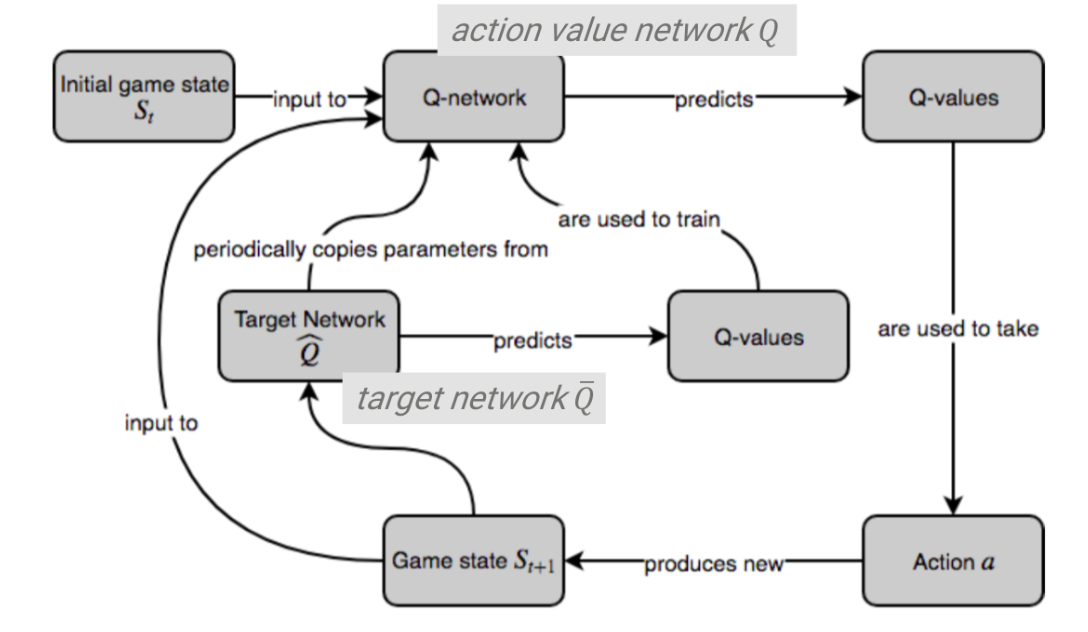
\includegraphics[scale=0.35]{captures/DeepQLearning.png}
	\caption{Esquema Método Deep Q-Learning. Extraída de origen. \cite{book:barto} \cite{article:RLromero}}
	\label{fig:deepqlearning} % Unique label used for referencing the figure in-text
	%\addcontentsline{toc}{figure}{Figure \ref{fig:GDS}} % Uncomment to add the figure to the table of contents
\end{figure}

En el apartado \ref{sec:qlearning} se habló de las ventajas de tener dos políticas en lugar de una, eso se mantiene. La diferencia de todo esto es que buscamos las actualizaciones de los dos conjuntos de pesos de ambas políticas en lugar de cambiar valores en una función-tabla. \\

\begin{verbatim}
for i={0,...,n_episodios}
   for t={0,...,n_entrenamiento}

      Elegir acción con política generadora de experiencia
      Aplicar acción y obtener estado siguiente y recompensa
      Almacenar estado, acción, recompensa y estado siguiente en memoria D

      Muestrear un mini-batch de experiencias de tamaño n_batch de la memoria D
      Obtener salida de predicción de cada experiencia usando política objetivo
      Optimizar red generadora de experiencia con gradiente descendente

      Cada C iteracciones , actualizar red objetivo a partir de la generadora
        de experiencia
\end{verbatim}

Al igual que hablamos de \textit{Double Q-Learning}, existe el \textbf{Double DQN}, tratando de mejorar el inconveniente de \textbf{sobreajuste} muy común en los métodos basados en valor, ya que la política objetivo elige siempre ese máximo. También existen otras propuestas como el uso de la \textbf{ventaja} visto en el apartado \ref{sec:ventaja}, junto con otras muchas variaciones de esta estrategia, aunque no son objetivo de este trabajo.

\section{Métodos basados en política: REINFORCE}

En los métodos basados en valor, el objetivo principal era aprender a evaluar las políticas, minimizando la diferencia o perdida entre el valor predicho y el valor objetivo. \\

Por otro lado, en los \textbf{Métodos basados en política} o \textbf{métodos de política gradiente} tratamos de optimizar directamente una política parametrizada, obteniendo una \textbf{distribución de probabilidades} del espacio de acciones. Para ello utilizamos una política de gradientes. \\

\begin{figure}[H]
	\centering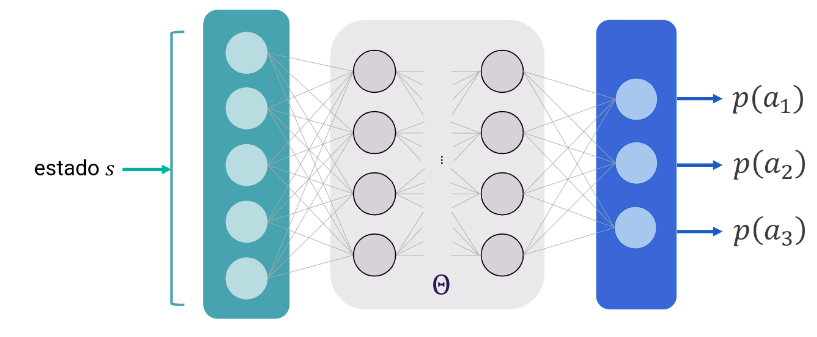
\includegraphics[scale=0.4]{captures/basadopolitica.png}
	\caption{Metodología basada en políticas. Extraída de origen. \cite{article:RLromero}}
	\label{fig:reinforce} % Unique label used for referencing the figure in-text
	%\addcontentsline{toc}{figure}{Figure \ref{fig:GDS}} % Uncomment to add the figure to the table of contents
\end{figure}

La principal ventaja que nos ofrece esta metodología es el hecho de que no suponga un inconveniente el \textbf{espacio de acciones} del problema. Si teníamos que elegir el valor máximo entre muchas estimaciones(una por cada acción), antes había que estimar cada una de ellas. Si había muchas acciones posibles(o esa acción es continua), la cantidad de estimaciones también era realmente alta, y por lo tanto, limitaba bastante a DQN en problemas de ese tipo. Mucha de la información calculada no era utilizada realmente. \\

Los métodos basados en política, por otro lado, pueden aprender más fácilmente esas \textbf{políticas estocásticas}, lo cual deriva en otros tipos de ventajas. Como aprender mejor de entornos parcialmente conocidos o no ser tan dependiente de la \textbf{suposición de Markov}. Además, no hay ese exceso de información que mencionábamos. \\

Estos métodos también suelen \textbf{converger más rápidamente} que los basados en valor, ya que fijamos directamente los parámetros de la red neuronal y estos se van modificando suavemente con los gradientes, por lo que nos aseguramos alcanzar, como mínimo, una \textbf{optimización local}. Los métodos basados en valor suelen ser algo más impredecibles en ese sentido.\\

El algoritmo REINFORCE tradicional se basa en una red neuronal la cual es entrenada \textbf{al final de cada episodio} con los valores que devuelve \textbf{Montecarlo} y que ya conocemos, calculando su valor de pérdida y optimización a partir de estos, utilizando el optimizador Adam mencionado en el apartado \ref{sec:optimizacion}.

\begin{align*}
&U(\Theta)=\sum_xP(x;\Theta)R(x)\\
&\nabla_\Theta U(\Theta) \approx \frac{1}{K}\sum^K_{i=1}\sum^n_{t=1}\nabla_\Theta log_{\pi_\Theta}(A^{(i)}_t|S^{(i)}_t)R(x^{(i)})
\end{align*}

$U(\Theta)$ es conocida como la función ``\textbf{máximo beneficio}'' es la que estamos tratando de maximizar. Generamos $K$ trayectorias $x^{(i)}$ de longitud $n$ según la política $\pi_ \Theta$. Calculamos la recompensa $R^i$ por cada una de las trayectorias y actualizamos el conjunto de pesos $\Theta$ para estimar el gradiente de esa función de máximo beneficio de la que hablábamos. \\

Existen muchas variantes como VPG aunque, de nuevo, no es el objetivo de este trabajo.\\

\begin{verbatim}
While no resuelto
    Generar K trayectorias de longitud n según política
    Calcular recompensa obtenida para cada trayectoria
    Actualizar pesos de la red para estimar el gradiente de la
      función "Máximo beneficio"
\end{verbatim}

\subsection{Proximal Policy Optimization(PPO2)}

Proponen una nueva familia de métodos de \textbf{gradiente de políticas} para el aprendizaje por refuerzo , que alternan entre el muestreo de datos a través de la interacción con el entorno(experiencia) y la optimización de una función objetivo mediante el \textbf{ascenso de gradiente estocástico}. \\

Mientras que los métodos estándar de gradiente de políticas realizan una actualización de los pesos en la red neuronal por muestra de datos, se propone una \textbf{función objetivo más novedosa} que organizan esas actualizaciones y múltiples épocas en mini-bath o mini-lotes, es decir, por \textbf{aproximación}. \\

Para esta técnica, se utiliza los valores de ventaja (apartado \ref{sec:ventaja}), la política antigua se ejecuta durante un periodo T(menos de un episodio) en la que se estima esos valores de ventaja. Cuando finaliza, optimiza los pesos de la política en épocas organizadas en \textit{mini-batches} y finalmente se sustituye esta política nueva por la antigua. \\

Esta estrategia presenta un buen equilibrio entre calidad de las actualizaciones de sus parámetros con el tiempo de aprendizaje. Supera a otros métodos de gradiente de políticas online, muestra por muestra, incluyendo además mejoras de simplicidad en la implementación y más generalizables en su uso. \\

Estos métodos son fundamentales para los avances actuales en el uso de redes neuronales profundas para el control y aprendizaje por refuerzo de locomoción 3D y \textit{Go}, entre otros. Sin embargo, supone un \textbf{desafío} porque presentan una sensibilidad notable a la elección del tamaño de esos periodos T y tamaños de los \textit{mini-batches} anteriormente mencionados. Demasiado pequeño, y el aprendizaje es inconvenientemente lento. Demasiado grande, y la señal se ve demasiado afectada por el ruido(exploración). \\

Una diferencia importante entre PPO y PPO2 en los baselines de OpenAI, es que el segundo incorpora una implementación de \textbf{activación de GPU}. Esto hace que el aprendizaje se produzca unas \textbf{tres veces más rápido} que en el PPO estándar, siempre que haya disponibilidad de recursos para explotarlo. \\

Además, esta versión incluye una variante de la función objetivo que es muy novedosa debido a que no se se suele encontrar en otros algoritmos. Implementa una forma de actualizar la política compatible con el gradiente descendente estocástico, mientras que simplifica el algoritmo eliminando la perdida de KL, la cual tiene propagación hacia atrás y es costosa, y la necesidad de realizar actualizaciones adaptativas. \\

Como vemos en su pseudocódigo, es sorprendentemente sencillo para lo que es capaz de hacer. \cite{article:PPO2_1} \cite{article:PPO2}

\begin{verbatim}
for i=1,2... 

   for actor=1,2,...
      Ejecutar política antigua en entorno durante T time-steps
      Calcular el valor de ventaja estimadas durante T
   
   Optimizar la función objetivo con K épocas y batch-sizes de tamaño M
\end{verbatim}

\section{Métodos actor-critic}

Llegados a este punto, conocemos los métodos basados en valor y basados en políticas. Sabemos cuales son las ventajas principales de cada uno de ellos. No obstante, vamos a centrarnos en los inconvenientes de cada uno.

De forma resumida, REINFORCE se basa en \textbf{actuar}, ya que calcula las probabilidades de todas las acciones para que nos conduzcan a un buen resultado final. Esto tiene un principal inconveniente, si una trayectoria conduce a un mal resultado final, puede \textbf{contener buenas acciones} que no están siendo reforzadas en su actualización de pesos(recordemos que se actualiza al final de cada episodio). \\

Por otro lado, DQN se centra en \textbf{estimar} los valores de recompensas que nos vamos a encontrar en el futuro a partir de un estado o estado-acción realizada en el entorno. El principal inconveniente de éste es que calcula las estimaciones a partir de estimaciones, lo cual introduce \textbf{sesgo} en el aprendizaje. \\

La propuesta que se va a analizar a continuación es una \textbf{combinación de las dos anteriores}, de ahí su nombre \textbf{actor-critic}(una parte actúa y la otra estima). Entonces, hace uso de dos redes: \\

\begin{itemize}
	\item \textbf{Actor:} Trata de seleccionar la mejor acción posible para el estado en el que se encuentra.\\
	
	\item \textbf{Critic:} Indica la estimación de recompensa acumulada que se espera a partir del estado actual ($V(S;\Theta_\upsilon)$) \\
\end{itemize}

La principal ventaja es que \textbf{acelera} el aprendizaje, al mismo tiempo que \textbf{evita sesgos} en sus estimaciones, por lo que lo hace más estable.

\begin{figure}[H]
	\centering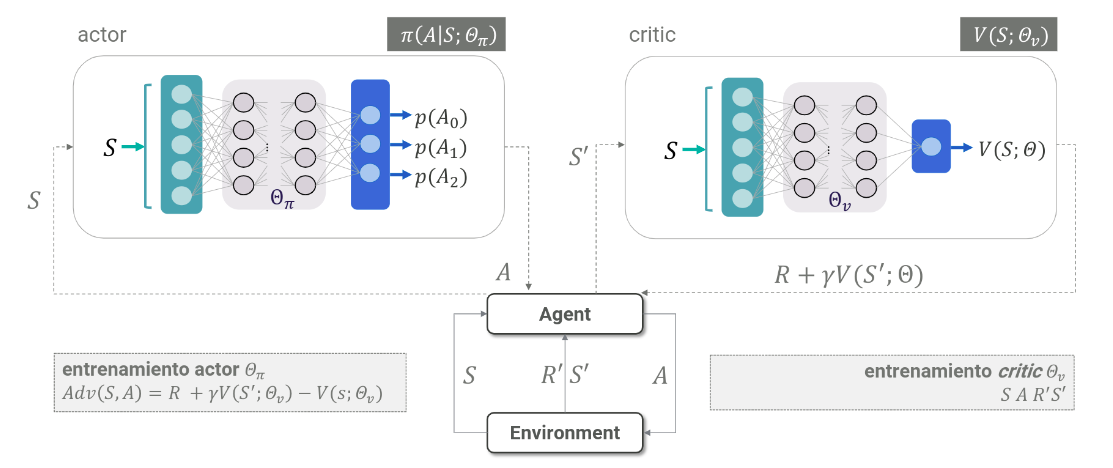
\includegraphics[scale=0.4]{captures/actorcritic.png}
	\caption{Esquema de metodología actor-critic. Extraída de origen. \cite{article:RLromero}}
	\label{fig:actorcritic} % Unique label used for referencing the figure in-text
	%\addcontentsline{toc}{figure}{Figure \ref{fig:GDS}} % Uncomment to add the figure to the table of contents
\end{figure}

El actor recibe un estado $s$, que a su vez provoca una acción $a$ por parte el mismo. Esa acción es realizada en el entorno, transitando a un estado nuevo $s'$, ese estado es analizado por el crítico el cual realiza la estimación, recogida por el agente de nuevo. \\

Lo más importante es que el actor aprende teniendo en cuenta las estimaciones del crítico, el cual aprende de forma directa utilizando las encuaciones de Bellman vistas en el apartado \ref{sec:bellman}. La explicación detallada de esta técnica depende directamente del algoritmo concreto que estemos hablando como, por ejemplo, A3C (aprendizaje asíncrono) o A2C(aprendizaje síncrono), aunque no entraremos en mayor detalle.

\subsection{Deep Deterministic Policy Gradient(DDPG)}

Este es un algoritmo que combina las técnicas de actor-critic junto con DQN. No es posible aplicar Q-Learning directamente a un problema con espacio de acciones continuo, es imposible hacer estimaciones de todo ese espacio. \\

Entonces, se propone una arquitectura actor-critic en la cual la parte crítica es DQN en lugar de $V(s;\Theta)$ (se estima Q). Para ello se utiliza una \textbf{memoria de experiencias} al igual que en la propia DQN. \\

Se dispone de un \textbf{actor} el cual se rige por una política $\pi(s;\Theta_\pi)$, en lugar de estimar la probabilidad de cada acción, devuelve directamente la acción seleccionada(un valor numérico de $a$). \\

La parte crítica es la función $Q$, puede hacerse para un espacio de acciones continua como se ilustró en la figura \ref{fig:RNcontinua}. El único inconveniente es que no se puede estimar el espacio de acciones A en su totalidad, dado que es infinito. \\

Al no tener valores de V, se ajusta directamente para maximizar Q obtenido con una acción y con esa información se entrena la red actor. \\

Ambas redes son dobles, como DQN, haciendo las actualizaciones más suaves con la ayuda de una red objetivo(\textit{target}), propias de los métodos \textit{off-policy}.\\

Esto tiene una ventaja para la \textbf{exploración}. Puede tratar el problema de exploración independientemente del algoritmo de aprendizaje. Se introduce \textbf{ruido} en los pesos de la red directamente, en lugar del espacio de acciones:

\begin{equation*}
\pi'(S_t)=\pi(S_t;\Theta_\pi)+N
\end{equation*}

Siendo N la representación del ruido añadido en esos parámetros.\\

\begin{figure}[H]
	\centering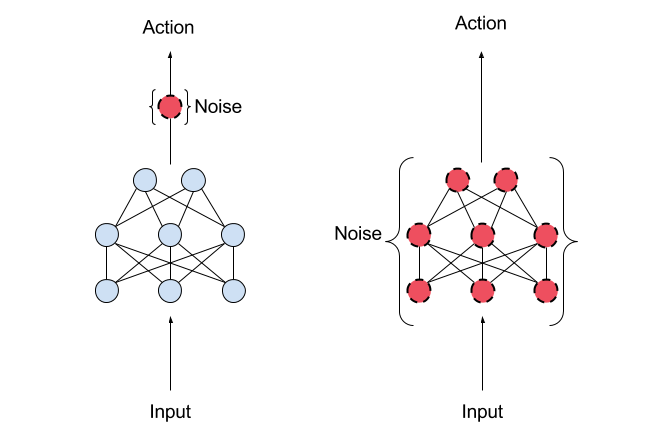
\includegraphics[scale=0.5]{captures/noise.png}
	\caption{Ruido en el espacio de acciones (izquierda) frente a ruido en los parámetros de la red (derecha). Extraída de origen. \cite{article:DDPG_2}}
	\label{fig:noise} % Unique label used for referencing the figure in-text
	%\addcontentsline{toc}{figure}{Figure \ref{fig:sigmoide}} % Uncomment to add the figure to the table of contents
\end{figure}

Esta técnica ha demostrado mejorar la exploración de los agentes obteniendo mejores resultados. Introducir ruido en los parámetros provoca que la exploración sea consistente a través del paso del tiempo, mientras que agregar el ruido en el espacio de acción conduce a una exploración \textbf{más impredecible} que no esta correlacionada con los parámetros \\

¿Cuánto y cómo se modifica esos pesos de la red? Los investigadores tienen que enfrentarse a tres problemas principales: \\

\begin{enumerate}
	\item Diferentes niveles de la red neuronal tienen \textbf{diferentes sensibilidades}. \\ 
	
	\item La sensibilidad de los pesos de la política también puede variar dependiendo del \textbf{progreso del aprendizaje} por el que se encuentre el agente, siendo más difícil predecir las repercusiones que tendrán cambiar sus pesos. \\ 
	
	\item Escoger la correcta escala de ruido es bastante complicado, ya que entender cómo influye en las decisiones del agente la modificación de esos parámetros es una tarea prácticamente imposible, las redes neuronales sirven para dar respuesta, no para describir cómo piensa el agente. \\
\end{enumerate}

Se usa normalización en las capas para solventar el primer problema, situando a todos los parámetros en una escala unificada. En cuanto al segundo y tercer problema, se combate utilizando una \textbf{planificación adaptativa}. \\

Consiste en determinar el rango modificable de los parámetros en función de su espacio de valores. Funciona midiendo la perturbación en la toma de decisiones del agente dado los parámetros y por tanto, definiendo de una forma automática cómo pueden ser variados. \cite{article:DDPG} \cite{article:DDPG_2}

\begin{verbatim}
Iniciar aleatoriamente la red crítica y actor con un conjunto de pesos diferentes.
Iniciar la red objetivo para la parte crítica
Iniciar una memoria de experiencia

for episodio i=1,...,T

   Iniciar proceso aleatorio de ruido N 
   Recibir estado inicial de la observación
   
   for t=1,...,T
   
      Seleccionar acción acorde con la política actor y el ruido de exploración
      Ejecutar acción y obtener recompensa y estado siguiente
      Almacenar tupla de experiencia en memoria
      Muestrear un mini-batch de N transiciones de la memoria de experiencia
      Obtener etiqueta aproximada con red objetivo
      Actualizar crítico minimizando función de perdida
      Actualizar actor utilizando política de gradientes estocástica
      
      Actualizar la red objetivo

\end{verbatim}

%Aquí hay una definición de recomensa, recompensa acumulada y estimación de recompensa que quizás es muy interesante de poner.

%\section{Técnicas}\label{sec:tectnicasRL}
%
%A continuación, vamos a ver algunas de las técnicas de aprendizaje por refuerzo más utilizadas. Todo ello, desde un punto de vista teórico y conceptual.
%
%\subsection{Política de gradientes}\label{sec:politicaGradientes}
%
%Como se menciona en el apartado \ref{sec:RL}, normalmente estas técnicas se usaran para mejorar un agente ya funcional, y no para crear uno desde cero. Normalmente, estos agentes que se usan como puntos de partida suelen ser redes neuronales supervisadas que han sido entrenadas a partir de información de otros agentes resolviendo esos problemas en el mismo entorno o, aprendiendo de las decisiones que tomaron los propios humanos. \\
%
%Llegados a este punto, nos encontramos ante un agente constituido por una red neuronal con unos \textbf{pesos o parámetros} explícitos en las conexiones entre capas, fruto del entrenamiento que ha tenido. Modificar estos pesos implica cambiar el comportamiento y naturaleza del agente ante el problema que resuelve, es como cambiar o modificar su cerebro e inteligencia. \\
%
%Podríamos modificar estos pesos ligeramente de forma aleatoria, para ver si encontramos un agente mejor que el actual. Esto generalmente es inviable, ya que estas técnicas se suelen utilizar en problemas demasiado complejos y amplios como para depender de la suerte en encontrar una buena combinación de pesos.\\
%
%En su lugar, podríamos analizar la experiencia que obtiene el agente al desenvolverse en el entorno con la finalidad de analizar y determinar cuales son los pesos que deberíamos modificar. Esta es la idea que trata de plasmar  la \textbf{política de gradientes}. A rasgos generales, su funcionamiento es simple. Una vez el agente termina un episodio: \\
%
%\begin{itemize}
%	\item Modifica los pesos de tal manera que \textbf{baja} la probabilidad de las jugadas que ha realizado a lo largo de la partida, si ha llegado a un estado terminal de \textbf{fracaso}. \\
%	
%	\item Modifica los pesos de tal manera que \textbf{sube} la probabilidad de las jugadas que ha realizado a lo largo de la partida, si ha llegado a un estado terminal de \textbf{éxito}. \\
%\end{itemize}
%
%Obviamente, una misma acción puede ser buena o mala dependiendo de la \textbf{situación} en la que nos encontremos. Cuando decimos que modificamos la probabilidad de que el agente realice una acción, nos referimos a que realice esa acción en situaciones iguales o parecidas en las que se encontraba en ese episodio. \\
%
%Modificamos entonces, los pesos del agente para que tenga ese comportamiento a la hora de estimar las probabilidades, no las probabilidades en sí de forma manual, ya que no tendrá sentido al solo tener efecto cuando se encontrara en exactamente la misma situación.\\
%
%La forma en la que el agente entiende una \textit{situación similar} viene intrínseca en las redes neuronales y en como abstrae conocimientos y patrones del entorno, cosa que como ya mencionamos en el apartado \ref{sec:introduccion}, no podemos explicar de forma clara al tener un conjunto de pesos enormes. \\
%
%No es una ciencia exacta, quiero decir, que haya tenido éxito en su objetivo final no quiere decir que todas las decisiones que ha tomado sean buenas. Ni que, en caso de no alcanzar el objetivo, todas las decisiones que ha tomado sean malas. Pero si es cierto que al hacer esto generalmente vamos a mejorar más de lo que empeoramos. \\
%
%Igualmente, este es el concepto base. Organizaciones de investigación punteras como DeepMind están constantemente trabajando sobre estas arquitecturas tratando de que sean más ricas y más acertadas. Por ejemplo introduciendo el concepto de discounting que mencioné en el apartado \ref{sec:experiencia}, entre muchas otras. \\
%
%Una de las formas de mejorar más importantes que se han descubierto en este ámbito es la \textbf{asignación de crédito}. Consiste en detectar de algún modo las \textbf{decisiones más relevantes} de cada episodio y utilizar esas para optimizar los pesos del agente. Es uno de los problemas más relevantes del aprendizaje por refuerzo, ya que cuento mejor sea la estrategia a seguir, mejor aprenderá el agente de su propia experiencia. \\
%
%Para actualizar estos pesos utiliza los \textbf{gradientes descendentes} de una forma muy similar a lo que explicamos resumidamente en el apartado \ref{sec:optimizacion}. Solo que en lugar de utilizar una etiqueta de aprendizaje supervisado para calcular la función de perdida, usamos la recompensa que se obtiene en la experiencia y optimizamos los pesos con esos valores. 
%
%\section{Q-Learning}\label{nfreofner}
%
%El \textbf{Q-Learning} o \textbf{aprendizaje por refuerzo con método de valores} toma un enfoque distinto al de política de gradientes explicado hace un momento. Imaginemos lo siguiente, cuando un comentarista de una partida de ajedrez dice la frase ``las blancas van algo mejor que las negras'', no es un concepto preciso. El comentarista, a través de toda la experiencia que él mismo tiene sobre ese entorno, puede hacer ciertas predicciones de quién está mejor colocado en el tablero y, por tanto, estimar que las blancas tienen más probabilidades de ganar que las negras en ese momento(de cumplir su objetivo en el entorno). \\
%
%Ese es el enfoque de esta técnica. El agente tiene la capacidad de \textbf{estimar} cuánta recompensa espera conseguir en el futuro a partir del estado actual del entorno. Ya no usaríamos una metodología de asignación de recompensas estática, como el método de \textbf{discounting} mencionado en el apartado \ref{sec:experiencia}, sino que en su lugar tendríamos un agente que utiliza esa misma experiencia para hacer su propia asignación de recompensas a sus propias acciones, y cada vez lo haría mejor. \\
%
%La función que nos devuelve esta recompensa estimada se define matemáticamente como $Q(s,a)$, de ahí su nombre de \textit{Q-learning}. La \textit{s} representa el estado del entorno actual y la \textit{a} representa la acción que se está considerando para realizar sobre \textit{s}. \\
%
%Para definir esta función Q se hace uso de las \textbf{redes neuronales} (\textbf{Deep Q-learning}). El comienzo es el mismo que en la política de gradientes. El agente recolecta los estados, acciones y recompensa de los episodios(experiencia). La diferencia se produce llegado a este punto. La forma en la que esta metodología actualiza el comportamiento del agente a partir de la experiencia recolectada consiste en sustituir la política de gradientes por esta función y probar todas las acciones posibles (dominio de \textit{a}) en el estado actual del entorno (\textit{s}). Se realizará la acción que haya devuelto un mejor resultado en la función. \\
%
%Pero recordemos que el aprendizaje por refuerzo premia mucho la \textbf{exploración}, por lo que no está mal que el agente de forma ocasional realice jugadas que el no haría normalmente, como mencionamos en el apartado \ref{sec:probabilidades} para que él mismo experimente qué pasaría si lo hace y aprenda de nuevas acciones buenas o acciones que son malas.
%
%%hacer esquema de Q-learning
%
%\section{Método actor-critic}\label{sec:actorcritic}
%
%El aprendizaje por refuerzo actor-critic, o actor-crítico traducido al español, maneja una morfología de aprendizaje que los humanos utilizamos en muchas ocasiones a lo largo de nuestra vida sin darnos cuenta. Con ella, aprendemos y mejoramos en muchos aspectos. \\
%
%Solemos supervisar, evaluar y, sobretodo, escuchar a individuos que son mejores que nosotros haciendo o desenvolviéndose en algo específico. Esta técnica trata de mezclar los puntos fuertes tanto de la \textbf{política de gradientes}(apartado \ref{sec:politicaGradientes}) como del método \textbf{Q-Learning} (apartado \ref{sec:qlearning}): \\
%
%\begin{itemize}
%	\item La política de gradientes hace de \textbf{actor}, ya que dado un estado del entorno decide la distribución de probabilidades de las distintas acciones que puede realizar para saber cuales de ellas son mejores y, por tanto, más seguras de que realice. \\
%	
%	\item La función de valor \textit{Q} hace de \textbf{crítico}. Decide cuando el actor mencionado en el punto anterior está tomando buenas o malas decisiones y, por consiguiente, cuando está más cerca de cumplir su objetivo o cuando se esta alejando del mismo respectivamente. \\
%\end{itemize}
%
%La información que aporta el crítico es fundamental para el proceso de entrenamiento del agente, del mismo modo que los consejos de un profesor podrían guiar nuestro propio estudio en algo y hacerlo más eficiente.\\
%
%Digamos que, por un lado, el actor aprende a realizar aquellas acciones que el crítico indica que son más prometedoras. Por otro lado, el crítico va mejorando también a la hora de estimar esas recompensas de las acciones que realiza. \\
%
%Un concepto esencial que debemos conocer cuando estemos hablando de esta técnica es la \textbf{ventaja}. Explicaremos a continuación cual es su significado y el por qué de su relevancia. \\
%
%\subsection{Ventaja}
%
%Ya vimos lo que era la \textbf{asignación de crédito} en el apartado \ref{sec:politicaGradientes}, el cual era un problema a resolver y mejorar fundamental para que estas técnicas de aprendizaje por refuerzo fueran cada vez mejores y más eficientes utilizando la experiencia recolectada. \\
%
%Cuando el agente consigue su objetivo. ¿Reforzamos todas las decisiones que ha tomado? Esto no es una buena idea. Si se tratase de un juego en el que nos enfrentamos a un rival, como GO, podría darse el caso de que nuestro contrincante no sea muy habilidoso y no haya sabido aprovechar las malas jugadas que ha realizado el agente. Mientras que nuestro entrenamiento está reforzando esas jugadas indiscriminadamente. \\
%
%Entendemos la \textbf{ventaja} como una fórmula para estimar la relevancia de una decisión(acción) en el resultado final conseguido. Para entender cómo podría estimarse esa relevancia, una vez más, nos fijamos en como lo hacemos nosotros mismos, como si nos mirásemos en un espejo. \\
%
%Imagina una partida de baloncesto. Un triple en el cuarto tiempo cuando el resultado es 78-80 supone un enorme cambio en el posible resultado final del partido. Sin embargo, si el resultado ya es 110-80, el triple carece de interés para los espectadores y muy difícilmente les emocione a pesar de que la ejecución es la misma. \\
%
%Este es el concepto principal en el cual gira esta técnica de estimación. Parece ser que las acciones más relevantes tienden a suceder en los momentos en los que el resultado final aún \textbf{permanece en duda}. La ventaja trata de desarrollar este concepto para el beneficio del propio agente que construimos.\\
%
%Primero, necesitamos una función que defina el \textbf{valor de un estado}. Es decir, cómo de favorable o desfavorable es la situación del entorno para el cumplimiento del objetivo del agente. Se denominará con $V(s)$. Es parecido al Q-learning explicado en el apartado \ref{sec:qlearning}, pero se limita a evaluar el estado del tablero(\textit{s}), no la relevancia de una acción en ese estado(no se tiene en cuenta \textit{a}). \\
%
%Entonces, introducimos este nuevo concepto junto con el Q-learning , de tal modo que la ventaja sería :
%
%\begin{equation*}
%A = Q(s,a) - V(s)
%\end{equation*}
%
%El problema de esto es definir \textit{Q}, ya que necesita de una red neuronal aparte y entrenarla para que estime el valor de las acciones en el entorno. Lo cual puede ser muy costoso y un problema añadido. Una posible solución podría sustituir la estimación \textit{Q} por la recompensa final del entorno una vez finaliza el episodio:
%
%\begin{equation*}
%A = R - V(s)
%\end{equation*}
%
%Lo que está haciendo el agente es calcular al mismo tiempo tanto su \textbf{función de estimación del valor} como la \textbf{función de su política}. \\
%
%\begin{itemize}
%	
%	\item Al principio de la partida, $V(s)$ normalmente valdrá 0. Esto es lógico, ya que un estado inicial del entorno no será más o menos favorable para el agente. Si al final cumple su objetivo, R tendrá un valor de 1(positivo), por lo que la ventaja de la primera acción será $1-0=1$. \\
%	
%	\item Imaginemos que el entorno está a punto de llegar a un estado terminal y que el agente las tiene todas consigo para cumplir su objetivo, por lo que $V(s)$ tiene un valor de $0.95$. Si, en efecto, el agente gana la partida, la ventaja de este movimiento será $1-0.95=0.05$. \\
%	
%	\item Imagina la misma situación pero, en lugar de cumplir el objetivo, el agente acaba fracasando. Entonces, la recompensa final sería de -1(negativa). En ese caso la ventaja adquiere un valor de $-1-0.95=-1.95$. \\
%	
%\end{itemize}
%
%En los primeros movimientos al aún no haberse decidido nada, la ventaja tiende a mantenerse neutra. Sin embargo, cuando el agente tiene una situación ventajosa y mete la pata o, por el contrario, si el agente tiene ya muy pocas posibilidades de alcanzar su objetivo y consigue revertir la situación, la ventaja se dispara de forma negativa y positiva respectivamente. \\
%
%En definitiva, hay que prestar atención en esos \textbf{cambios bruscos} del valor de la ventaja que se pueden producir en el transcurso de cada decisión que toma el agente. Son en esas decisiones en las que debemos tener mayor consideración a la hora de establecer una guía para la actualizaciones de los pesos de nuestro agente. Cuanto más \textbf{bruscos} sea el cambio de la ventaja, más relevantes serán esas decisiones, ya sea positiva o negativamente.
%
%\begin{figure}[H]
%	\centering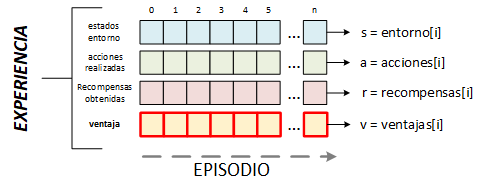
\includegraphics[scale=1]{captures/experiencia2.png}
%	\caption{La ventaja se incluye en la experiencia, pero es introducida al final del episodio, cuando ya se sabe todas las recompensas.}
%	\label{fig:experiencia2} % Unique label used for referencing the figure in-text
%	%\addcontentsline{toc}{figure}{Figure \ref{fig:sigmoide}} % Uncomment to add the figure to the table of contents
%\end{figure}

%------------------------------------------------

%----------------------------------------------------------------------------------------
%	PART 3
%----------------------------------------------------------------------------------------

\part{Desarrollo y Experimentación}

\section*{Introducción}\label{sec:introduccionexp}

Hasta ahora, hemos explicado desde un punto de vista más \textbf{teórico} los conceptos que vamos a manejar durante el desarrollo de este trabajo. Ahora, daremos un enfoque \textbf{práctico} de todo el esfuerzo que se ha dedicado en este proyecto. Las explicaciones serán realizadas a partir de entornos específicos. \\

Utilizaremos para ello las librerías de \textbf{OpenAI} para aplicar estos algoritmos en \textbf{Python} y algunos entornos de \textbf{Gym} en los que le daremos la posibilidad a nuestros agentes de ``ensayar'' su tareas. \\

Por experiencia, las redes neuronales son computacionalmente costosas en términos generales, sin contar con las técnicas de aprendizaje por refuerzo que utilizaremos. Por ello, se hará uso de una \textbf{máquina virtual}, aprovechando los \textbf{recursos en la nube} para contar con una mayor potencia y, por tanto, reducir los tiempos de entrenamientos necesarios para nuestros agentes. Utilizaremos la plataforma de \textbf{Google Cloud}. \\

Por último, veremos el resultado final. La eficacia del funcionamiento de los agentes obtenidos junto con los resultados de la monitorización de su aprendizaje. Estos datos serán mostrados, analizados y extraeremos las conclusiones de este proceso y objetivo final conseguido.

\chapterimage{openai-logo.png}
\chapter{OpenAI baselines}\label{sec:DRL}

Las técnicas DRL vistas en el capítulo anterior serán usadas e ilustradas de las librerías de \textbf{OpenAI}. Se trata de un laboratorio de investigación con sede en San Francisco, California. Su misión y línea de trabajo general consiste en utilizar la inteligencia artificial en beneficio de la humanidad. No solamente por ellos, sino por cualquiera, ya que brindan sus algoritmos, técnicas e implementaciones de código abierto a cualquiera que tenga la voluntad y la curiosidad para realizar sus propias investigaciones. \cite{article:openAI}. \\

Podemos ver los avances que han obtenido en su página web \cite{article:openAI2}, siendo en general sobre inteligencia artificial, pero sobretodo relacionada con aprendizaje por refuerzo y redes neuronales.\\

%Explicar por qué se ha elegido los baselines y no otras opciones como Rlib

Es una de las últimas propuestas para crear una estandarización de las implementaciones de algoritmos DRL. Sin embargo, no es la única que existe, es difícil decidir cuál es la mejor librería de todas las posibles. Se pueden encontrar otras alternativas como \textit{RLlib}, \textit{Stable Baselines}, \textit{TersorForce}, \textit{KerasRL}... Entre otras cuantas más. \\

Uno de los principales motivos por los que se ha elegido a \textit{OpenAI baselines} es su comunidad activa, la documentación y detalles de los algoritmos que implementa y la incorporación de ejemplos sencillos con la finalidad de facilitar el entendimiento de uso a los más nuevos. \\

Sus implementaciones están desarrolladas en Python, el cual es un lenguaje muy potente y ha demostrado buen desempeño en otros campos de IA, sin mencionar la legibilidad de su código y lo fácilmente modificable que resulta. Además, incluye funcionalidad propia para la recogida de información del proceso de entrenamiento y librerías para el tratamiento y visualización de la misma. \\

La compatibilidad con entornos Gym y la gran variedades de adaptaciones de otros entornos hace que sea muy abarcable con una gran cantidad de problemas, incluso de algunos que no han sido desarrollado por la propia OpenAI, lo veremos más adelante. \\

Por último, destacar su estado del arte, teniendo un gran abanico de los algoritmos más novedosos, aunque en este trabajo solo se vaya a analizar varios de ellos.

%\section{Algoritmos}\label{sec:Algoritmos}
%
%Los algoritmos que hemos utilizado han sido extraídos y analizados de \textbf{OpenAI baselines} en Github. Es un conjunto de implementaciones de alta calidad de algoritmos de aprendizaje por refuerzo y por refuerzo profundo. \cite{article:baselines} \\
%
%Estos algoritmos, a disposición del público, hacen que sea más fácil para la comunidad de investigadores replicar, refinar e identificar nuevas ideas, creando la base para trabajar con ellas. Incluso siendo utilizadas como método de comparación con otras técnicas de aprendizaje mas tradicionales. Tratan de situarse a la par con los trabajos más punteros en la actualidad. Sin embargo, tal y como se puede apreciar en su repositorio, tienen un constante mantenimiento tanto para mejorar como para solucionar ciertos errores que van surgiendo con su desarrollo. Por lo que, en ocasiones, nos podemos encontrar ante técnicas o entornos de uso que no terminan de ser estables del todo, ya hablaremos de ello más adelante. \\
%
%Son herramientas las cuales también se favorecen de las aportaciones de la comunidad, estando forkeada unas 3300 veces, por lo que a veces podemos encontrarnos ciertos problemas a la hora de utilizarlos y tendremos que solventarlos para conseguir el objetivo que buscamos. Conforme nos encontremos en el contexto adecuado explicaré mi experiencia personal de uso y como solventé los problemas que a mí personalmente me fueron surgiendo.
%
%\subsection{PPO2}\label{sec:PPO2}
%
%Es el acrónimo de \textbf{Proximal Policy Optimization}, junto con el número que denota una reimplementación del mismo ante su versión original en baselines. \\
%
%Proponen una nueva familia de métodos de \textbf{gradiente de políticas} para el aprendizaje por refuerzo , que alternan entre el muestreo de datos a través de la interacción con el entorno(experiencia) y la optimización de una función objetivo mediante el \textbf{ascenso de gradiente estocástico}. \\
%
%Por consiguiente, sería un algoritmo desarrollado a partir de los apartados \ref{sec:politicaGradientes} y \ref{sec:deeplearning}, junto con una de las optimizaciones vistas en \ref{sec:optimizacion}. \\
%
%Mientras que los métodos estándar de gradiente de políticas realizan una actualización de los pesos en la red neuronal por muestra de datos, se propone una \textbf{función objetivo más novedosa} que organizan esas actualizaciones y múltiples épocas en mini-bath o mini-lotes. \\
%
%Como ya mencionamos, esta estrategia hace que tengamos un buen equilibrio entre calidad de las actualizaciones de sus parámetros con el tiempo de aprendizaje. Supera a otros métodos de gradiente de políticas en línea, muestra por muestra, incluyendo además mejoras de simplicidad en la implementación y más generalizables en su uso. \\
%
%Estos métodos son fundamentales para los avances actuales en el uso de redes neuronales profundas para el control y aprendizaje por refuerzo de locomoción 3D y \textit{Go}, entre otros. Sin embargo, supone un \textbf{desafío} porque presentan una sensibilidad notable a la elección del tamaño de pasos o actualizaciones que debe realizar. Demasiado pequeño, y el aprendizaje es inconvenientemente lento. Demasiado grande, y la señal se ve demasiado afectada por el ruido(exploración). \\
%
%Con estos problemas podríamos darnos de narices ante una caída catastrófica y repentina en la eficacia del agente. Como inconveniente general, necesitan millones o miles de millones de actualizaciones para aprender tareas simples, lo que supone recabar mucha experiencia; ensayos y errores. Por lo que estas técnicas no pueden ser utilizadas para cualquier tipo de problema, es dependiente de su complejidad. \\
%
%Los investigadores han tratado de compensar estos defectos con algoritmos como \textit{ACER} o \textit{TRPO}(también disponibles en los baselines de Github) intentando restringir u optimizar de alguna manera el tamaño de las actualizaciones de política(pesos). \\
%
%No obstante, \textit{ACER} es mucho más complicado que \textit{PPO2}, cuando solo ha sido demostrado funcionar mejor con \textit{Atari}. Por otro lado, \textit{TRPO} no es fácilmente compatible con algoritmos que comparten parámetros entre una política y una función de valor o pérdidas auxiliares. Es decir, método \textit{actor-critic} visto en el apartado \ref{sec:actorcritic}. \\
%
%Una diferencia importante entre PPO y PPO2 en los baselines de OpenAI, es que el segundo incorpora una implementación de \textbf{activación de GPU} que nos es muy útil dado nuestro entorno de trabajo que explicaremos en el apartado \ref{sec:infraestructura}. Esto hace que el aprendizaje se produzca unas \textbf{tres veces más rápido} que en el PPO estándar, siempre que tengamos los recursos para poder aprovecharlo claro. \\
%
%Además, esta versión incluye una variante de la función objetivo que es muy novedosa debido a que no se se suele encontrar en otros algoritmos. Implementa una forma de actualizar la política compatible con el gradiente descendente estocástico, mientras que simplifica el algoritmo eliminando la perdida de KL, la cual tiene propagación hacia atrás y es costosa, y la necesidad de realizar actualizaciones adaptativas. \\
%
%Esto hace que tenga un buen rendimiento y muy parecido a ACER en Atari, a pesar de ser mucho más sencillo que éste. Podemos ver algunos videos de ejemplo funcionando para problemas de control continuo, como hacer caminar un robot en un entorno simulado, en las referencias utilizadas. \cite{article:PPO2_1} \cite{article:PPO2}
%
%\subsection{DQN}\label{sec:DQN}
%
%Este algoritmo es el resultado de utilizar la técnica de \textbf{Q-Learning} explicada en el apartado \ref{sec:qlearning} implementada en una \textbf{red neuronal profunda}, apartado \ref{sec:deeplearning}.  \\
%
%Esto permite que esa técnica Q-Learning, perteneciente al aprendizaje por refuerzo, pueda ser viable y funcionar bien en entornos más complejos, de mayor dimensionalidad, como podrían ser los videojuegos o robótica. \\
%
%OpenAI ha hecho un gran trabajo con este algoritmo, ya que tiene un \textbf{sistema de repetición}. Si no he entendido mal su funcionamiento, consiste en revisar la experiencia junto con las recompensas estimadas por DQN, de tal manera que puede comprobar donde la recompensa real difiere de la estimada de forma significativa, permitiendo al agente reajustarse en función de suposiciones realizadas de forma errónea por su parte. En otras palabras, es una manera de \textbf{reproducir sus recuerdos} para aprender de ellos una vez se han producido las consecuencias a posteriori. \\
%
%Al combinar Q-learning con una red neuronal, siendo un trabajo concreto de ingeniería por parte de OpenAI, esta técnica presenta alguna diferencia de las vistas anteriormente en este trabajo por separado. Explicado de una forma esquematizada; divide la red neuronal en dos partes: \\
%
%\begin{enumerate}
%	\item Una parte aprende a proporcionar una \textbf{estimación del valor} a cada paso del agente, define como de buena es su situación en ese momento. \\
%	
%	\item La otra calcula las \textbf{ventajas potenciales de cada acción} realizada, sería la parte más familiar por nosotros comentada hasta el momento. \\
%	
%\end{enumerate}
%
%Ambas partes se \textbf{combinan} de una forma concreta, de tal manera que obtenemos un \textbf{único valor} como salida de la red. \cite{article:DQN}
%
%\subsection{DDPG}\label{sec:DDPG}
%
%Esta es la adaptación de la técnica de \textbf{actor-critic} vista en el apartado \ref{sec:actorcritic}. Aquí el dominio de acciones a realizar por el agente debe ser \textbf{continuo} y no discreto, por la naturaleza del propio algoritmo. Esto nos dará problemas en el futuro que deberemos resolver, lo veremos en un momento más apropiado a lo largo de esta documentación. \\
%
%Un concepto que debemos tener muy en cuenta para esta técnica será el \textbf{parámetro de ruido}. Esto hace referencia al concepto de introducir algo de \textbf{aleatoriedad} al agente como ya explicamos en el apartado \ref{sec:probabilidades} \\
%
%Cuando mencionamos esa distribución de probabilidades entre las distintas posibles decisiones o acciones del agente, en realidad mencionamos la forma ``tradicional'' de hacerlo, ya que introducíamos el ruido directamente en el espacio de acciones del agente para conseguir esa \textbf{aleatoriedad dirigida} que mencionábamos. \\
%
%Este algoritmo introduce el ruido de una forma \textbf{más novedosa}, ya que \textbf{modifica de forma directa} los parámetros de la red neuronal sobre la que se monta DDPG. \\
%
%Esto altera de forma leve la política del agente, y por tanto, las decisiones que tomará, pero solo dependiendo de la situación actual en la que se encuentre (input en ese momento). Recordemos que esta técnica se combina con Q-Learning que estima como de prometedor es el futuro del agente, y ahí no estamos introduciendo ruido. \\
%
%En resumen, introducimos \textbf{aleatoriedad} a los pesos de las conexiones que tiene la red neuronal. Los pesos están fijados por la técnica de entrenamiento a la que ha estado sujeta el agente hasta ese momento, pero esos pesos pueden ser modificados de forma leve a la hora de utilizar dicha red para tomar una decisión.
%
%\begin{figure}[H]
%	\centering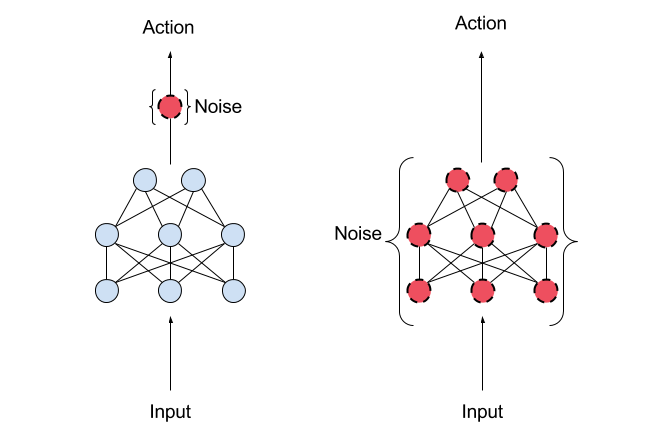
\includegraphics[scale=0.5]{captures/noise.png}
%	\caption{Ruido en el espacio de acciones (izquierda) frente a ruido en los parámetros de la red (derecha). Extraída de origen. \cite{article:DDPG_2}}
%	\label{fig:noise} % Unique label used for referencing the figure in-text
%	%\addcontentsline{toc}{figure}{Figure \ref{fig:sigmoide}} % Uncomment to add the figure to the table of contents
%\end{figure}
%
%Esta técnica ha demostrado mejorar la \textbf{exploración} de los agentes obteniendo finalmente mejores resultados y comportamiento más elegantes, entendiendo por elegantes a decisiones o estrategias más parecidas al comportamiento humano. \\
%
%Se cree que introducir ruido en los parámetros provoca que la exploración sea consistente a través del paso del tiempo, mientras que agregar el ruido en el espacio de acción conduce a una exploración \textbf{más impredecible} que no esta correlacionada con los parámetros (inteligencia) del propio agente. \\
%
%la idea esta clara, ¿pero cuánto y cómo modificamos esos pesos de la red exactamente? Los investigadores tienen que enfrentarse a tres problemas principales: \\
%
%\begin{enumerate}
%	\item Diferentes niveles de la red neuronal tienen \textbf{diferentes sensibilidades}. \\ 
%	
%	\item La sensibilidad de los pesos de la política también puede variar dependiendo del \textbf{progreso del aprendizaje} por el que se encuentre el agente, siendo más difícil predecir las repercusiones que tendrán cambiar sus pesos. \\ 
%	
%	\item Escoger la correcta escala de ruido es bastante complicado, ya que entender cómo influye en las decisiones del agente la modificación de esos parámetros es una tarea prácticamente imposible. Recordemos que una de las características de las redes neuronales es que \textbf{no podemos entender como toman sus decisiones} (apartado \ref{sec:introduccion}) \\
%\end{enumerate}
%
%Se usa normalización en las capas para solventar el primer problema, situando a todos los parámetros en una escala unificada. En cuanto al segundo y tercer problema, se combate utilizando una \textbf{planificación adaptativa}. \\
%
%Consiste en determinar el rango modificable de los parámetros en función de su espacio de valores. Funciona midiendo la perturbación en la toma de decisiones del agente dado los parámetros y por tanto, definiendo de una forma automática cómo pueden ser variados. \\
%
%Como conclusiones extraídas sobre el \textit{ruido}, considero que esta técnica \textbf{da mejores resultados} aunque es \textbf{más difícil} de afinar dado un problema. Cuando introducimos el ruido en el espacio de acciones, da peores resultados en general, pero es más simple de introducir y más interpretable dado que trabajamos directamente sobre las acciones que toma el agente. \cite{article:DDPG} \cite{article:DDPG_2}

\chapterimage{humanoid.png}
\chapter{Entornos Open AI Gym}\label{sec:entornos}

En este apartado, se va a explicar los problemas y \textbf{entornos} elegidos para el desarrollo del proyecto. \\

Podríamos utilizar los algoritmos explicados para resolver \textbf{problemas del mundo real}. Por desgracia, puede ser que en la mayoría de casos nos encontremos con una serie de inconvenientes que haga más complicado poder llegar siquiera a entrenar un agente. \\

Por una parte, está el \textbf{presupuesto}. Supongamos un agente que sea un robot humanoide y que el problema a resolver sea obtener la capacidad de correr en entornos hostiles(piedras, agujeros en el suelo, terrenos irregulares,etc.) a una buena velocidad y sin caerse o perder el equilibrio por parte del mismo. No sería nada barato tener un agente con los sensores y características suficientes, no estaría al alcance de cualquier persona. \\

Por otra parte, hay que tener en cuenta el \textbf{riesgo} que supone equivocarse en un entorno real. El riesgo en este caso, sería la posibilidad de que el robot se averíe en el momento que cometa errores que le hagan caer. \\

Por suerte, existe una alternativa. La respuesta a estos inconvenientes son los \textbf{entornos simulados}. Simular ese mismo entorno en un \textbf{mundo virtual} y entrenar esa inteligencia desde ahí, con un agente y sensores también virtuales. Normalmente las grandes compañías dedicadas a esto parten de esos entornos antes de probarlo con robots físicos en un entorno físico, lo cual les ahorra muchos errores, dinero y tiempo. \\

Existe, por ejemplo, un software que permite entrenar futuros sistemas de conducción automáticos desde el entorno creado en el videojuego de RockStars, \textit{Grand Theft Auto V}. Esto evitaría el riesgo de experimentar con peatones, vehículos e infraestructura urbana real. \\

\begin{figure}[H]
	\centering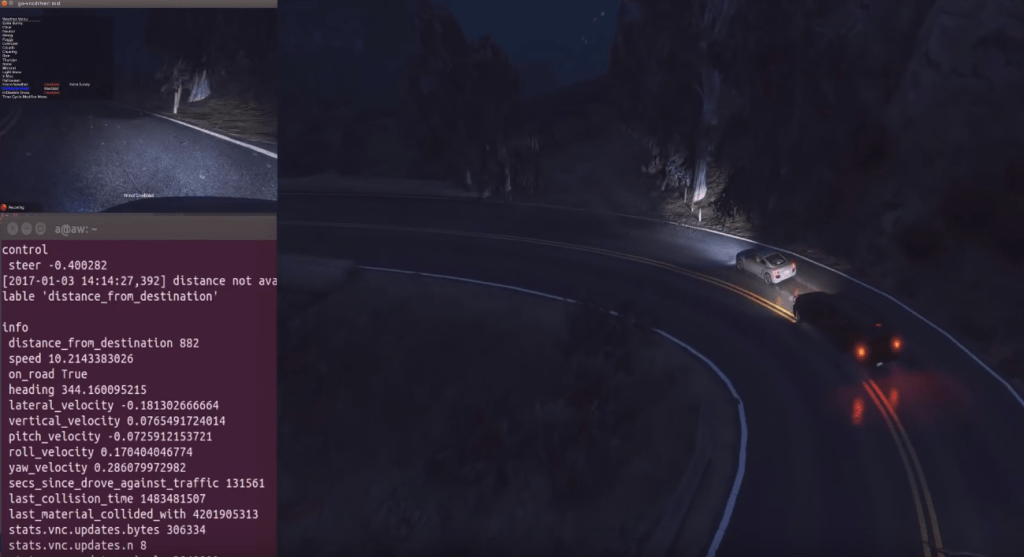
\includegraphics[scale=0.4]{captures/gta.png}
	\caption{Agente entrenando conducción autónoma en entorno simulado de GTA V. Extraída de vídeo en Youtube. \cite{article:gta}}
	\label{fig:gta} % Unique label used for referencing the figure in-text
	%\addcontentsline{toc}{figure}{Figure \ref{fig:sigmoide}} % Uncomment to add the figure to the table of contents
\end{figure}

En concreto, nosotros vamos a utilizar unos entornos predefinidos, de nuevo, por OpenAI. La librería que los implementa y ejecuta es llamada \href{https://gym.openai.com/}{Gym}. Se trata de un conjunto de herramientas desarrolladas en Python, al igual que los \textit{baselines}, que brinda soporte de entornos simulados de distintos tipos para que podamos realizar pruebas con nuestros agentes. \\

Hay una gran diversidad de entornos, algunos son muy simples, otros más complejos; algunos no son fieles al mundo real tratando de hacerlos más simples, y otros tratan de simular la realidad lo mejor posible. \\

En definitiva, vamos a trabajar con dos entornos, uno simple y otro algo más complejo, con los que probar y analizar las técnicas mencionadas en los apartados anteriores. \cite{article:gym} \cite{article:entornos}

\section{MountainCar-v0}\label{sec:mountaincar}

Este es un entorno muy sencillo y simple que nos va a permitir familiarizarnos tanto con los \textit{baselines} como con \textit{Gym}, entendiendo cómo funcionan y cómo se utilizan para crear nuestras propias pruebas y agentes con los métodos de aprendizaje por refuerzo profundo. \\

Una \textbf{carreta} se encuentra en una pista unidimensional, teniendo únicamente una dirección y sus dos sentidos como libertad de movimiento. La carreta se encuentra entre dos ``montañas''. El objetivo es conseguir subir a la montaña que se encuentra a su derecha. \\

El problema es sencillo, pero no tanto como llega a aparentar, resulta que el motor que tiene esa carreta \textbf{no es suficientemente potente} como para poder subir la cuesta de esa montaña. \\

Solo existe una forma de resolverlo; conduciendo de un lado a otro para conseguir generar el impulso suficiente o, dicho de otra forma, un mayor momento lineal o momentum con el que la carreta conseguirá subir hasta la cima. \\

La idea es partir de un agente que \textbf{sabe el objetivo}, pero \textbf{no cómo se consigue}, ya que solo se le proporcionará los datos que se recogen del entorno (input), las posibles salidas que puede realizar (outputs posibles) y las recompensas en función de las acciones que realice en cada momento(rewards). \\

\begin{figure}[H]
	\centering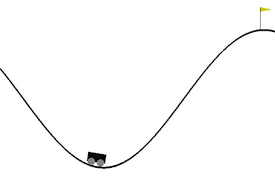
\includegraphics[scale=0.8]{captures/carreta.png}
	\caption{Representación gráfica del problema MountainCar v0 de OpenAI Gym.}
	\label{fig:carreta} % Unique label used for referencing the figure in-text
	%\addcontentsline{toc}{figure}{Figure \ref{fig:sigmoide}} % Uncomment to add the figure to the table of contents
\end{figure}

Podemos ver los detalles técnicos en el repositorio oficial de OpenAi para Gym en Github \cite{article:mountain2}. Las \textbf{observaciones} del entorno, o lo que es lo mismo, el \textit{input} que recibe el agente, es un contenedor con \textbf{dos datos} por observación: \\

\begin{itemize}
	\item \textbf{position}: Posición en la que se encuentra la carreta. Los valores que puede alcanzar se encuentran entre $-1.2$ y $0.6$ que correspondería a los límites de izquierda y derecha en la figura \ref{fig:carreta} respectivamente. \\
	
	\item \textbf{velocity}: Alcanza valores comprendidos entre $-0.07$ y $0.07$. Representa la velocidad de la carreta en esa observación. Si el valor es negativo sería en el sentido izquierdo y si es positivo en el sentido derecho. \\
\end{itemize}

Por otro lado, las \textbf{acciones} o decisiones posibles que puede tomar en cada \textit{time-step} son: \\

\begin{itemize}
	\item \textbf{0} $\rightarrow$ \textit{push left}: Esta acción representada por el valor 0 activa el motor de la carreta para que trate de moverse hacia la izquierda. \\
	
	\item \textbf{1} $\rightarrow$ \textit{no push}: Desde el momento en el que realiza esta acción el motor permanecerá apagado hasta que realice otra acción. \\
	
	\item \textbf{2} $\rightarrow$ \textit{push right}: Esta acción activa el motor de la carreta para que trate de moverse hacia la derecha. \\	
\end{itemize}

Que la acción sea \textit{push left} no quiere decir que en la observación siguiente esté moviéndose hacia la izquierda, ya que se tiene en cuenta, no solo el motor, sino la pendiente en la que se encuentra y la velocidad que tenía en ese momento. El entorno implementa esa \textbf{física básica} que habría en el mundo real. \\

Ahora hablemos de la \textbf{recompensa}. La \textbf{función de recompensa} podría ser pensada de diferentes formas. En este caso, se ha decidido que la recompensa para su entorno sea -1 en cada \textit{time-step} si no se encuentra en la meta y 1 en caso de alcanzarla. \\

También tenemos que hablar del \textbf{estado inicial} del entorno. Será con la carreta \textbf{sin velocidad} y en una posición aleatoria entre $-0.6$ y $-0.4$.\\

Se entiende como un \textbf{estado final} en el entorno cuando han ocurrido 200 \textit{timesteps} sin que la carreta haya alcanzado la meta o cuando la haya alcanzado en menos de esos 200 pasos. \\

%La carreta puede tardar más o menos pasos en conseguir su objetivo ¿Cuando se considera un resultado razonable? La suma de recompensas desde el estado inicial hasta el estado final del entorno siempre será 1 menos el número de pasos realizados por la carreta. Ya que cada paso resta 1 y solo suma 1 una vez alcanza la meta. \\

La recompensa acumulada, por tanto, será -200 cuando no consigue su objetivo y un valor negativo mayor que -200 cuando si lo alcanza. OpenAI Gym determina como \textbf{resultado satisfactorio} una recompensa total de -110 o mayor de media cada 100 episodios.\cite{article:mountain} \\

\section{MountainCarContinuous-v0}\label{sec:mountaincarcontinuo}

El problema planteado es exactamente igual que el anterior. La diferencia reside en que las acciones que el agente puede realizar no son discretas (\textit{push left}, \textit{push right} o \textit{no push}), sino continuas. \\

En otras palabras, la acción se representa con un \textbf{valor real}; siendo el 0 equivalente al \textit{no push}, valores positivos trata de mover la carreta hacia la derecha y valores negativos hacia la izquierda. \\

La otra diferencia reside en su definición de \textbf{función de recompensa}, siendo la recompensa acumulada igual al valor 100 menos la suma cuadrática de los \textit{time-steps} sucedidos hasta alcanzar la meta. Añadir un número máximo de \textit{time-steps} que pueden sucederse es altamente recomendable para evitar que suceda un episodio infinito en el que no logra alcanzar la meta. \\

Se considera como \textbf{resuelto} cuando se obtiene una media de recompensas por encima de 90 en los episodios. Este entorno ha sido utilizado específicamente para el algoritmo DDPG, recordemos que este algoritmo solo funciona con entornos continuos y no discretos, por lo que esta adaptación era necesaria.\cite{article:mountaincontinuous}.

\section{Super Mario Bros}

Es un famoso videojuego de plataformas, generalmente conocido. Fue diseñado por la compañía Nintendo en el año 1983 para la videoconsola Nintendo Entertainment System (NES). El objetivo es llegar al final de las fases que tiene prediseñadas sin ``morir'' antes, cada una de ellas con sus obstáculos y dificultades propias.\\

\begin{figure}[H]
	\centering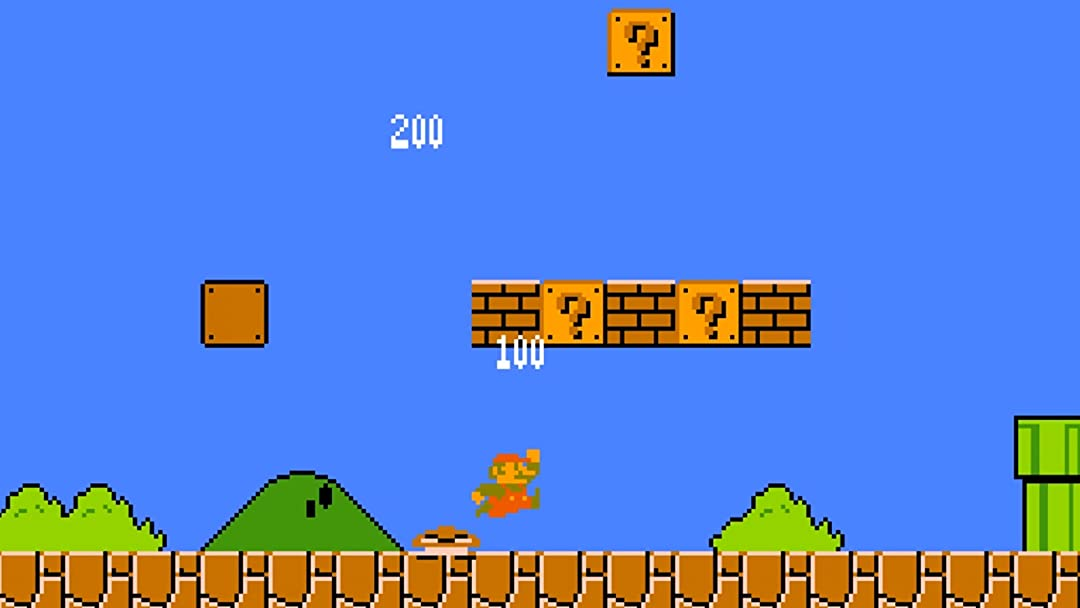
\includegraphics[scale=0.35]{captures/mario.jpg}
	\caption{Entorno del videojuego Super Mario Bros.}
	\label{fig:mario} % Unique label used for referencing the figure in-text
	%\addcontentsline{toc}{figure}{Figure \ref{fig:sigmoide}} % Uncomment to add the figure to the table of contents
\end{figure}

Este consta de una mayor complejidad que el entorno anterior; obstáculos, enemigos de distinto tipo, agujeros que saltar, tuberías por las que meterse... Por defecto, \textit{OpenAI baselines} no incorpora un entorno adaptado para su computación con técnicas DRL. Se ha hecho uso de la librería \textit{gym-retro}\cite{article:gymretro} para adaptarlo a este framework y programarlo bajo las mismas librerías que usamos para el problema anterior. Esta librería lo importa a partir de la ROM original de NES, la cual se puede descargar previamente. \\

Se han encontrado algunas dificultades para acceder a las especificaciones del entorno. Resulta que no hay mucha documentación sobre los entornos que se importan a través de \textit{gym-retro}, al menos no de forma directa. \\

Se accedió a las librerías de OpenAI, concretamente a las del archivo \textit{run.py} y fue modificado para que se obtuviera los datos de los estados por terminal:

\begin{figure}[H]
	\centering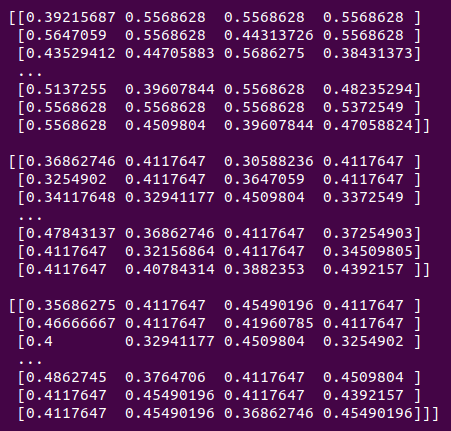
\includegraphics[scale=0.4]{captures/estado_mario.png}
	\caption{Entrada del agente en Super Mario Bros.}
	\label{fig:entradamario} % Unique label used for referencing the figure in-text
	%\addcontentsline{toc}{figure}{Figure \ref{fig:sigmoide}} % Uncomment to add the figure to the table of contents
\end{figure}

Por lo obtenido en la figura \ref{fig:entradamario}, da la sensación de que se trata una imagen con 3 canales de color(RGB) normalizados a valores entre 0 y 1(en lugar a 0 y 255 que corresponde a un byte). \\

Si observamos el código de gym-retro HIPERENLACE, existe una definición de las \textbf{observaciones} o estados del entorno. Pueden ser imágenes RGB o un volcado de RAM, parece que por defecto se utiliza imágenes RGB como se estaba comentando. \\

Si se hace memoria del apartado \ref{sec:convolucional}, sabremos que las mejores redes neuronales que se pueden utilizar por debajo para este problema son las CNNs. El tipo de red es seleccionable. Por defecto, es CNN para este entorno, aunque puede ser cambiado a otros tipos. \\

Entonces, estamos hablando de que el agente interpreta el entorno de una forma muy similar a los humanos. En lugar de tener un conjunto de variables estructuradas que define las observaciones, con información concreta, tiene una matriz con los valores RGB, siendo equivalente a observar la pantalla de la videoconsola directamente. Los humanos interpretamos esos valores de frecuencia como colores y el agente lo hace con valores numéricos, pero la filosofía es la misma. \\

Las \textbf{acciones} que puede hacer el agente son referentes únicamente al movimiento de Mario en el nivel:\\

\begin{itemize}
	\item Nada
	\item A
	\item B
	\item derecha
	\item derecha + A
	\item derecha + B
	\item derecha + A + B
	\item izquierda
	\item izquierda + A
	\item izquierda + B
	\item izquierda + A + B
	\item abajo
	\item arriba\\
\end{itemize}

Siendo A la acción de saltar y B la acción de esprintar/lanzar bola de fuego cuando Mario se encuentra en una situación que lo permite.\\

Las acciones son discretas, aunque algunas de ellas se obtienen combinando más de una acción. Por ejemplo, la acción derecha+A desencadena un salto al mismo tiempo que se desplaza a la derecha, dos acciones que se pueden realizar por separado y que el resultado no sería el mismo. \\

En este videojuego, los saltos pueden ser más prolongados o menos. Esto se consigue dejando pulsado el botón de salto(A) durante más tiempo. El tiempo se encuentra discretizado(t). Entonces, en este entorno tener la acción A establecida en más de un \textit{time-step} consecutivo, equivale a un salto prolongado. \\

El juego original funciona a 25 FPS's, lo cual significa que cada segundo de juego tenemos 25 frames o inputs. Estos frames van a ser muy similares entre ellos, tanto en estados,recompensas, o acción a realizar. Esto retrasa mucho el entrenamiento. Para simplificar este proceso, se realizá la omisión de frames estocásticos donde cada n-simo frame se utiliza como estado y las acciones son iguales a las anteriores con una probabilidad $p$ predefinida, para favorecer esas prolongaciones en los saltos, por ejemplo. Es una forma de tener menos datos con los que trabajar al mismo tiempo que no se compromete la eficacia del proceso de entrenamiento.\\

En cuanto a las \textbf{recompensas}, la función de recompensa acumulada es: 

\begin{equation*}
R=V+T+D+S
\end{equation*}

\begin{itemize}
	\item \textbf{V}: Es la diferencia de la posición del agente en la coordenada x entre estados. Cuanto más se desplace hacia la derecha, mejor. \\
	
	\item \textbf{T}: Es la diferencia del tiempo de juego entre frames. \\
	
	\item \textbf{D}: Es un valor que penaliza un agente cuando muere en un estado. Esto favorece a que el agente trate de no morir bajo ningún concepto. \\
	
	\item \textbf{S}: Es la diferencia de puntuación del juego entre frames. \\
\end{itemize}

Esta función asume que el objetivo del juego es moverse a la derecha, ya que la meta en todos los modelos de nivel se encuentra en esa dirección, tan rápido como sea posible, sin morir y obteniendo todos los puntos que pueda en el proceso. Es importante que cada uno de los valores que lo componen estén debidamente estudiados y escalados, ya que el agente puede encontrar una mejor opción en detenerse obteniendo puntos y tratar de llegar a la meta cuando apenas le queda tiempo restante. Es la importancia que ya se ha mencionado en más de una ocasión de definir el problema lo mejor posible para que el proceso de aprendizaje sea adecuado. \\

Es interesante que en el valor de recompensa acumulada no se especifique de forma implícita que debe llegar al final del nivel. Al tratar de maximizar todo lo posible esa función de recompensa, lo conseguirá de forma indirecta. \\

%Hablar de la otra posibilidad de coger la alternativa de gym directa con diccionario para el formato de entrada (más inetersante la que he utilizado yo)

Existen otras variantes del entorno de Super Mario Bros en Gym que pueden interpretar el problema de una forma distinta. Por ejemplo, en lugar de usar la imagen directamente, considerar un diccionario de información que define un estado del entorno de forma estructurada. En lugar de un conjunto de pixeles, estamos hablando de un conjunto de variables con la posición de Mario, enemigos, monedas, tiempo restante, vidas, etc.

\chapterimage{google-cloud.jpg}
\chapter{Entorno de desarrollo}\label{sec:cloud}

Tener a disposición una mayor cantidad de recursos para poder realizar una mayor cantidad de entrenamientos y pruebas de agentes en una menor cantidad de tiempo es un factor muy beneficioso para este proyecto. \\

Por ello, se tomó la decisión de utilizar \textbf{infraestructura de la nube}. Tras un análisis del mercado, se ha decidido utilizar \textbf{Google Cloud} para montar una máquina virtual que pudiéramos utilizar para entrenar y guardar agentes en los entornos explicados.\\

Existen un buen número de plataformas que nos ofrecen una gran diversidad de servicios en la nube de buena calidad. Los usuarios solo deben de preocuparse de usarlo(y pagar lo que corresponda), dejando el resto de ámbitos a la propia empresa que abastece. \\

Estos ámbitos son la administración de recursos, disponibilidad, integridad de los datos, etc. En muchos aspectos estarán, como organización, mejor preparados para dar los servicios. Por ejemplo, en cuestión de seguridad, con casi total certeza, serán más robustos y estarán mejor preparados que lo que puede estar un usuario de forma individual. \\

De forma general y resumida, podemos decir que \textbf{Google Cloud Platform} ofrece una mejor \textbf{potencia de procesamiento}, mientras que \textbf{Amazon Web Services}(AWS) destaca más en la \textbf{capacidad de memoria}. Para nuestro proyecto interesa que el servicio de procesamiento sea lo mejor posible, ya que para los entrenamientos que realizaremos serán esenciales. \\

Otro de los puntos fuertes de Google Cloud es la escalabilidad y equilibrio de carga que ofrece, que permite ajustar la infraestructura de una forma más exacta a nuestras necesidades. Los precios de Google son más competitivos, aunque ofrece menos servicios que AWS. En este caso, interesa mejores precios y menos servicios siempre que los necesarios se encuentren. \\

Para más detalles de su configuración y utilización, se encuentra en los apéndices de esta documentación(\ref{sec:googlecloud} y \ref{sec:usomaquina}).

\section{Metodología de experimentación}

La máquina cuenta con una mayor potencia, como es lógico, que un ordenador personal corriente. Sin embargo, tiene una desventaja. Al comunicarse por SSH desde una terminal, no se dispone de la interfaz gráfica(gnome de linux) que \textit{baselines} necesita para probar el agente de una manera visual. \\

Entrenamos los modelos y obtenemos los logs en la máquina virtual. Después, se traen de vuelta al equipo personal con el comando SCP para posteriormente visualizarlos desde la interfaz. El coste computacional viene casi en su totalidad en el entrenamiento, por lo que es el uso concreto que hacemos con los recursos en la nube.

\begin{figure}[H]
	\centering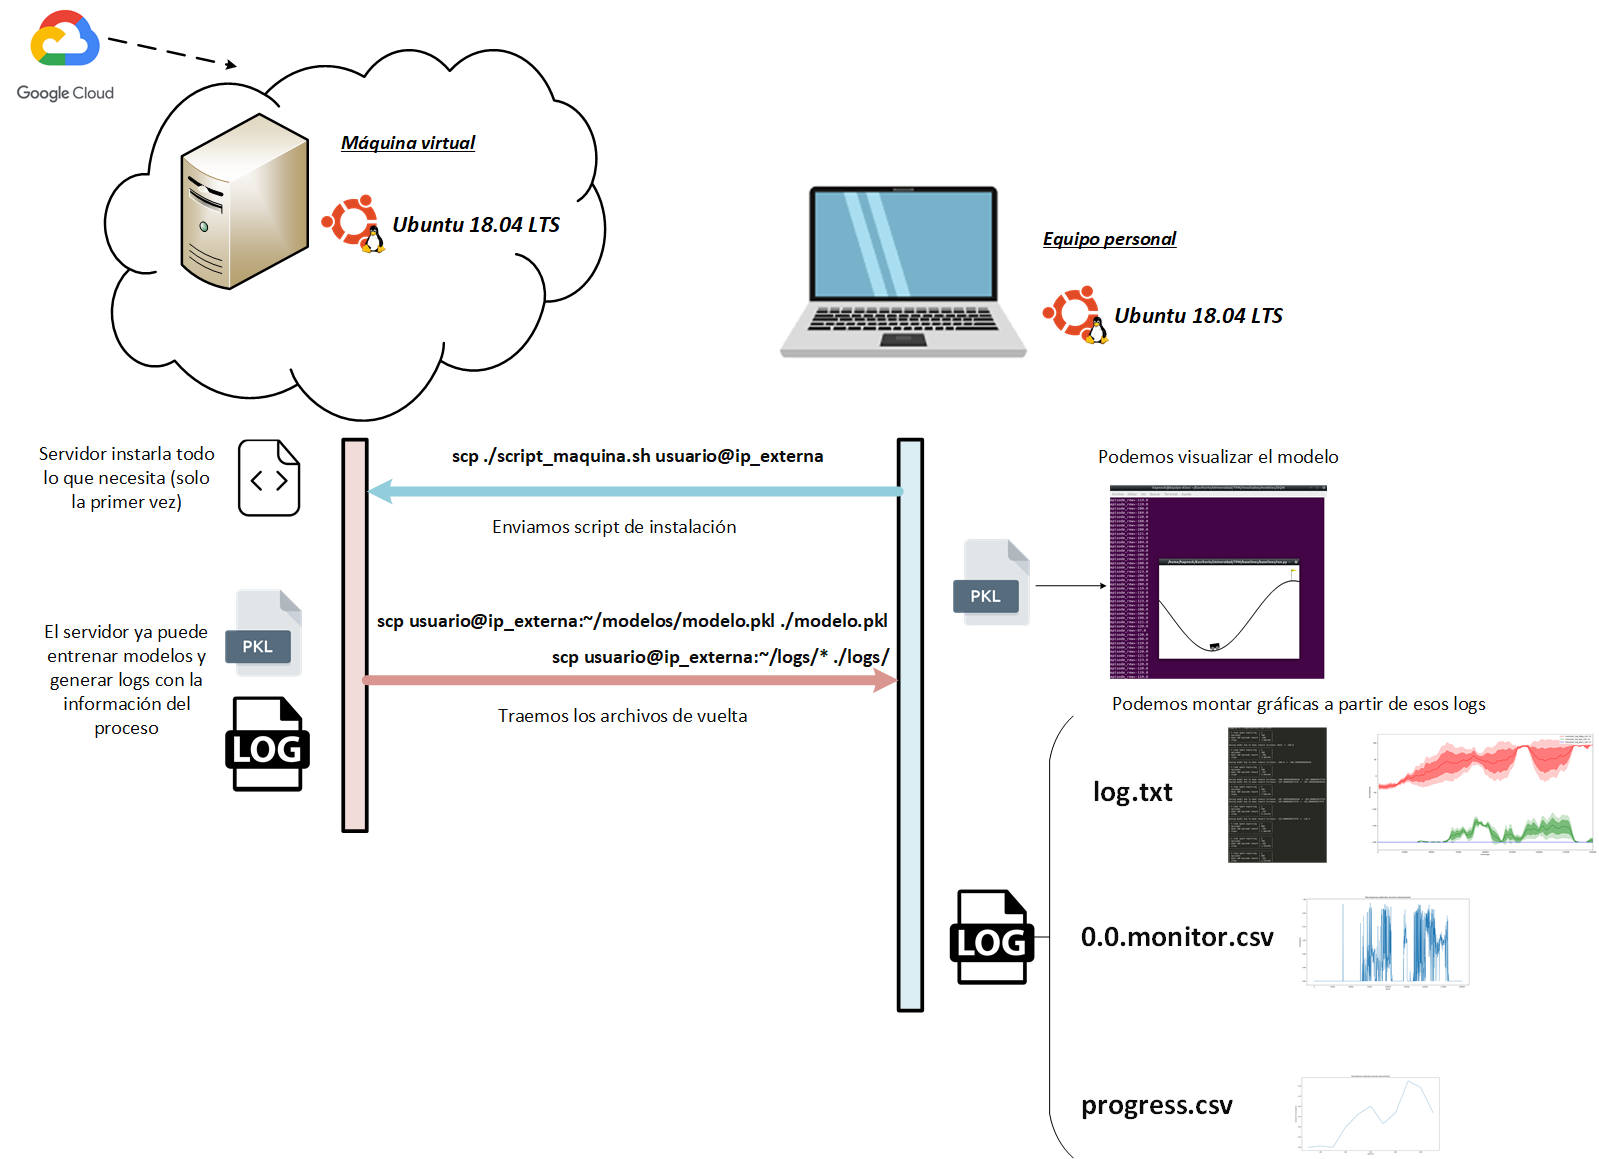
\includegraphics[scale=0.5]{captures/esquemaTrabajo.png}
	\caption{Esquema de metodología de trabajo entre mi equipo personal y la máquina virtual creada}
	\label{fig:formaTrabajo} % Unique label used for referencing the figure in-text
	%\addcontentsline{toc}{figure}{Figure \ref{fig:sigmoide}} % Uncomment to add the figure to the table of contents
\end{figure} 

\chapterimage{grafica.png}
\chapter{Experimentación: Resultados Obtenidos}

En este capítulo, vamos a mostrar y discutir sobre los resultados que hemos obtenido de los algoritmos, entornos de gym y entorno de trabajo que hemos explicado en este proyecto. \\

Para más información sobre los logs y su visualización en el proceso de aprendizaje de los agentes que veremos a continuación, se puede consultar el apéndice de esta documentación(\ref{sec:logs} y \ref{sec:visualizarlogs}).

\section{MountainCar-v0}

Se han obtenido una serie de modelos con las técnicas DQN, DDPG y PPO2. Todas ellas han sido entrenadas en un total de 2,5 millones de \textit{time-steps}, el número de episodios depende de cada ejecución. \\

Al tratarse de un problema con información estructurada en el input, se ha decidido utilizar una arquitectura de red multicapa, es decir, parte densa vista en la sección \ref{sec:deeplearning}. En baselines se define como tipo ``mlp'' y ya viene preconfigurada, por lo que no tenemos que preocuparnos por ello en principio. \\

A continuación se muestra en una tabla los resultados más relevantes obtenidos en estas pruebas.

\begin{table}[H]
	\begin{tabular}{c|l|l|l|l|}
		\cline{2-5}
		\multicolumn{1}{l|}{}                                                              & \textbf{\begin{tabular}[c]{@{}l@{}}media recompensa\\ (cada 100 ep)\end{tabular}} & \textbf{semilla}           & \textbf{\begin{tabular}[c]{@{}l@{}}episodios\\ transcurridos\end{tabular}} & tiempo (segundos)           \\ \hline
		\multicolumn{1}{|c|}{\cellcolor[HTML]{C7DCB4}}                                     & -149.40                                                                           & 3                          & 12600                                                                      & 6247                        \\ \cline{2-5} 
		\multicolumn{1}{|c|}{\cellcolor[HTML]{C7DCB4}}                                     & -113.10                                                                           & 13                         & 12800                                                                      & 6109                        \\ \cline{2-5} 
		\rowcolor[HTML]{C3D7FA} 
		\multicolumn{1}{|c|}{\multirow{-3}{*}{\cellcolor[HTML]{C7DCB4}\textbf{DQN}}}       & \textbf{-100.40}                                                                  & \textbf{113}               & \textbf{20600}                                                             & 5926                        \\ \hline
		\rowcolor[HTML]{C3D7FA} 
		\multicolumn{1}{|c|}{\cellcolor[HTML]{C7DCB4}}                                     & \textbf{94.30}                                                                    & \textbf{3}                 & \textbf{23400}                                                             & \textbf{6569}               \\ \cline{2-5} 
		\rowcolor[HTML]{FFFFFF} 
		\multicolumn{1}{|c|}{\cellcolor[HTML]{C7DCB4}}                                     & 94.27                                                                             & 13                         & 25700                                                                      & 6577                        \\ \cline{2-5} 
		\rowcolor[HTML]{FFFFFF} 
		\multicolumn{1}{|c|}{\multirow{-3}{*}{\cellcolor[HTML]{C7DCB4}\textbf{DDPG}}}      & {\color[HTML]{000000} 94.03}                                                      & {\color[HTML]{000000} 113} & {\color[HTML]{000000} 25800}                                               & {\color[HTML]{000000} 5248} \\ \hline
		\rowcolor[HTML]{C3D7FA} 
		\multicolumn{1}{|c|}{\cellcolor[HTML]{C7DCB4}{\color[HTML]{000000} \textbf{PPO2}}} & \textbf{-200}                                                                     & \textbf{113}               & \textbf{12500}                                                             & 1315                        \\ \hline
	\end{tabular}
\end{table}

Recordemos que el algoritmo DDPG funciona en \textit{MountainCarContinuous-v0} y que la función de recompensa y por tanto su rango de valores es diferente a DQN y PPO2. En cuanto a PPO2, solo se ha mostrado un resultado, porque en todos los experimentos ha ocurrido exactamente lo mismo; una recompensa de -200 (no alcanzar la meta nunca).\\

\subsection{DQN}

En DQN, la mayoría de semillas alcanzan una buena media de recompensas muy pronto y después comienzan a empeorar (semilla 3 y 13). No obstante, en la semilla 113, ocurre algo poco común; converge pronto pero se mantiene, incluso mejora poco a poco los resultados de recompensa hasta alcanzar la mejor recompensa obtenida en entrenamientos para esta técnica (-100). \\

%\begin{figure}[H]
%	\centering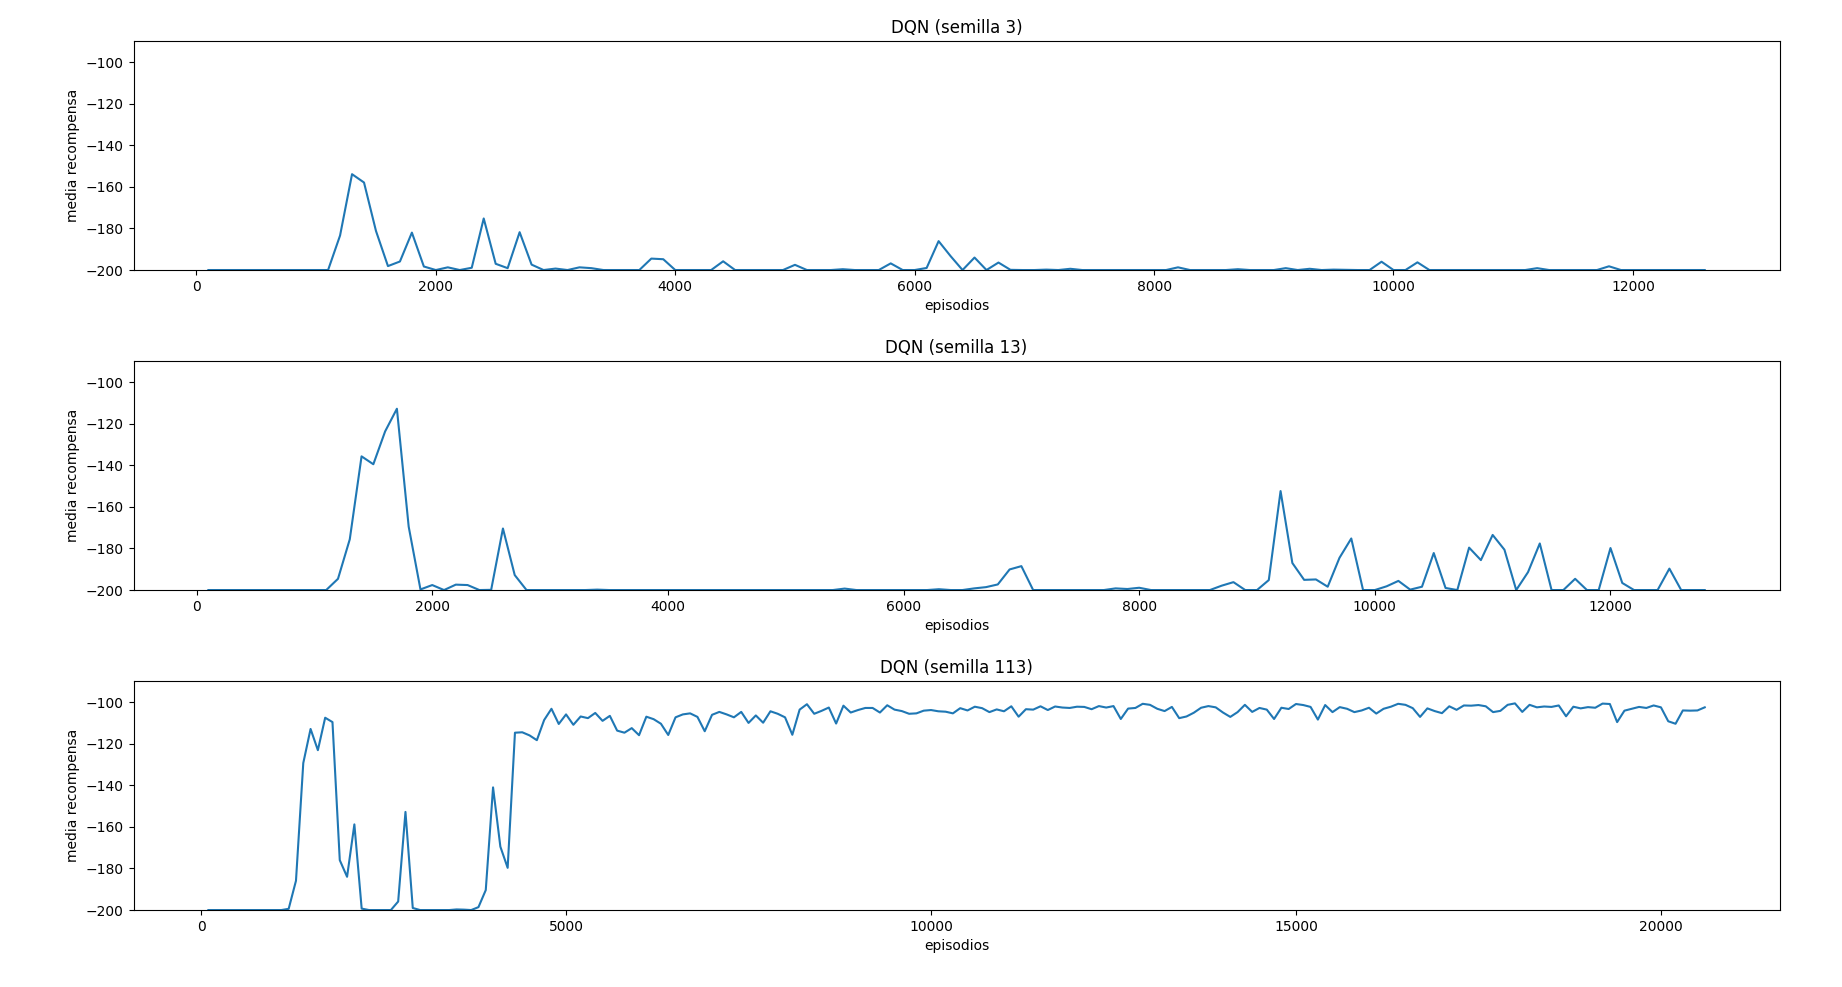
\includegraphics[scale=0.27]{mountain/mountain-dqn.png}
%	\caption{Media recompensas acumuladas cada 100 episodios.}
%	\label{fig:mountainDQN} % Unique label used for referencing the figure in-text
%	%\addcontentsline{toc}{figure}{Figure \ref{fig:sigmoide}} % Uncomment to add the figure to the table of contents
%\end{figure} 

\begin{figure}[H]
	\centering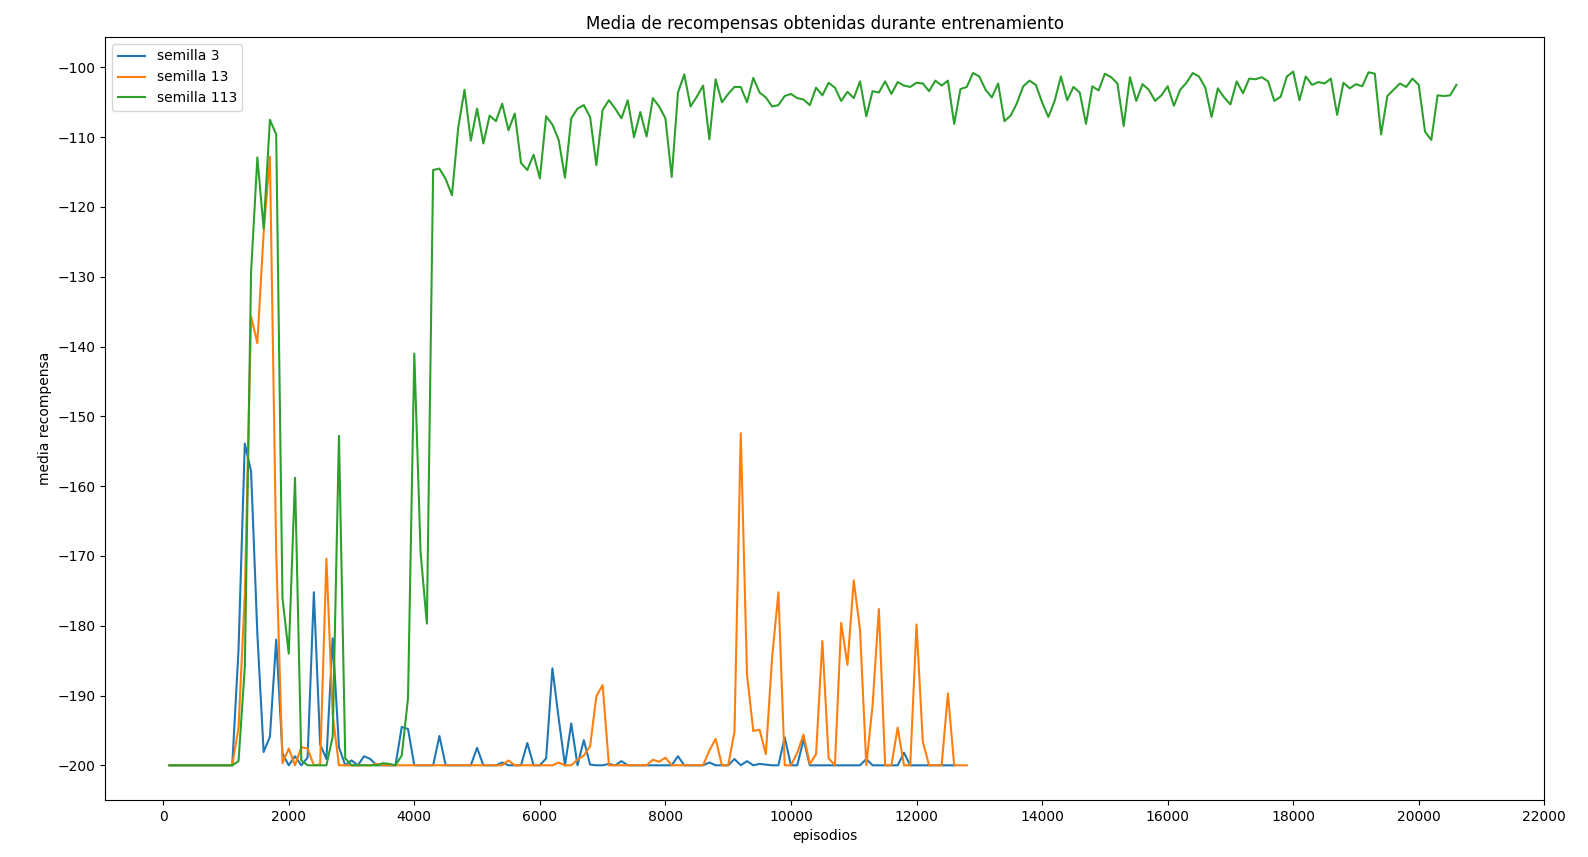
\includegraphics[scale=0.27]{mountain/mountain-dqn2.png}
	\caption{Media recompensas acumuladas cada 100 episodios, todas las semillas.}
	\label{fig:mountainDQN2} % Unique label used for referencing the figure in-text
	%\addcontentsline{toc}{figure}{Figure \ref{fig:sigmoide}} % Uncomment to add the figure to the table of contents
\end{figure} 

Por como está definido el problema, el número de episodios y la recompensa acumulada están relacionados. Cuanta mejor sea la recompensa de media, menos \textit{time-steps} por episodio. Al tener una duración de entrenamiento fija, esto se traduce en un mayor número de episodios. \\

La mayoría de modelos no alcanzan valores malos, siendo lo común encontrarnos recompensas comprendidas entre -140 y -110 (se han realizado entrenamientos con otras semillas diferentes de las mostradas), recordemos que una recompensa de -110 ya se considera un modelo totalmente eficaz. De forma extraordinaria, podemos dar con entrenamientos como en la semilla 113. No solo obteniendo una recompensa acumulada máxima más alta que el resto, sino capaz de mantenerse estable. \\

¿Por qué ocurre esto? A pesar de la apariencia, MountainCar es un problema complejo. La función de recompensa solo ofrece un valor positivo cuando alcanza la meta, siendo valores negativos en el resto de casos, esto es conocido como \textbf{sparse reward} y es un problema bastante frecuente en los problemas de aprendizaje por refuerzo. \cite{article:sparse} \\

Esto hace que sea muy complicado para el algoritmo lograr conectar series de acciones que sean beneficiosas para una recompensa acumulada futura. Si esa escasez de recompensas positivas es intratable, resultaría en un agente que nunca puede alcanzar el objetivo y aprender a representar una concatenación de acciones buena para el problema. Una solución posible a este inconveniente es entrenar con RL redes neuronales ya eficaces en cierta medida, en lugar de partir de cero. De hecho, es lo que hacen con AlphaStar, por ejemplo, entrenando a partir de modelos ya funcionales mediante aprendizaje supervisado de partidas de humanos, pero ya hablaremos de ello. \\

Otra solución podría ser elaborar otra función de recompensa que no tuviera este problema, lo que se traduce en un \textbf{cambio de definición} de ese problema. Proponer una función diferente puede influir y mucho en ese proceso de aprendizaje y cómo el agente consigue optimizarse. \\

Tener unas recompensas tan dispersas puede hacer que la exploración del agente se complique y no pueda llegar a converger. Por esa misma razón la aleatoriedad (semillas) influye tanto en los entrenamientos con esta técnica y la exploración, sobretodo al principio, es fundamental para tratar de encontrar esas recompensas que se necesitan. \\

\begin{figure}[H]
	\centering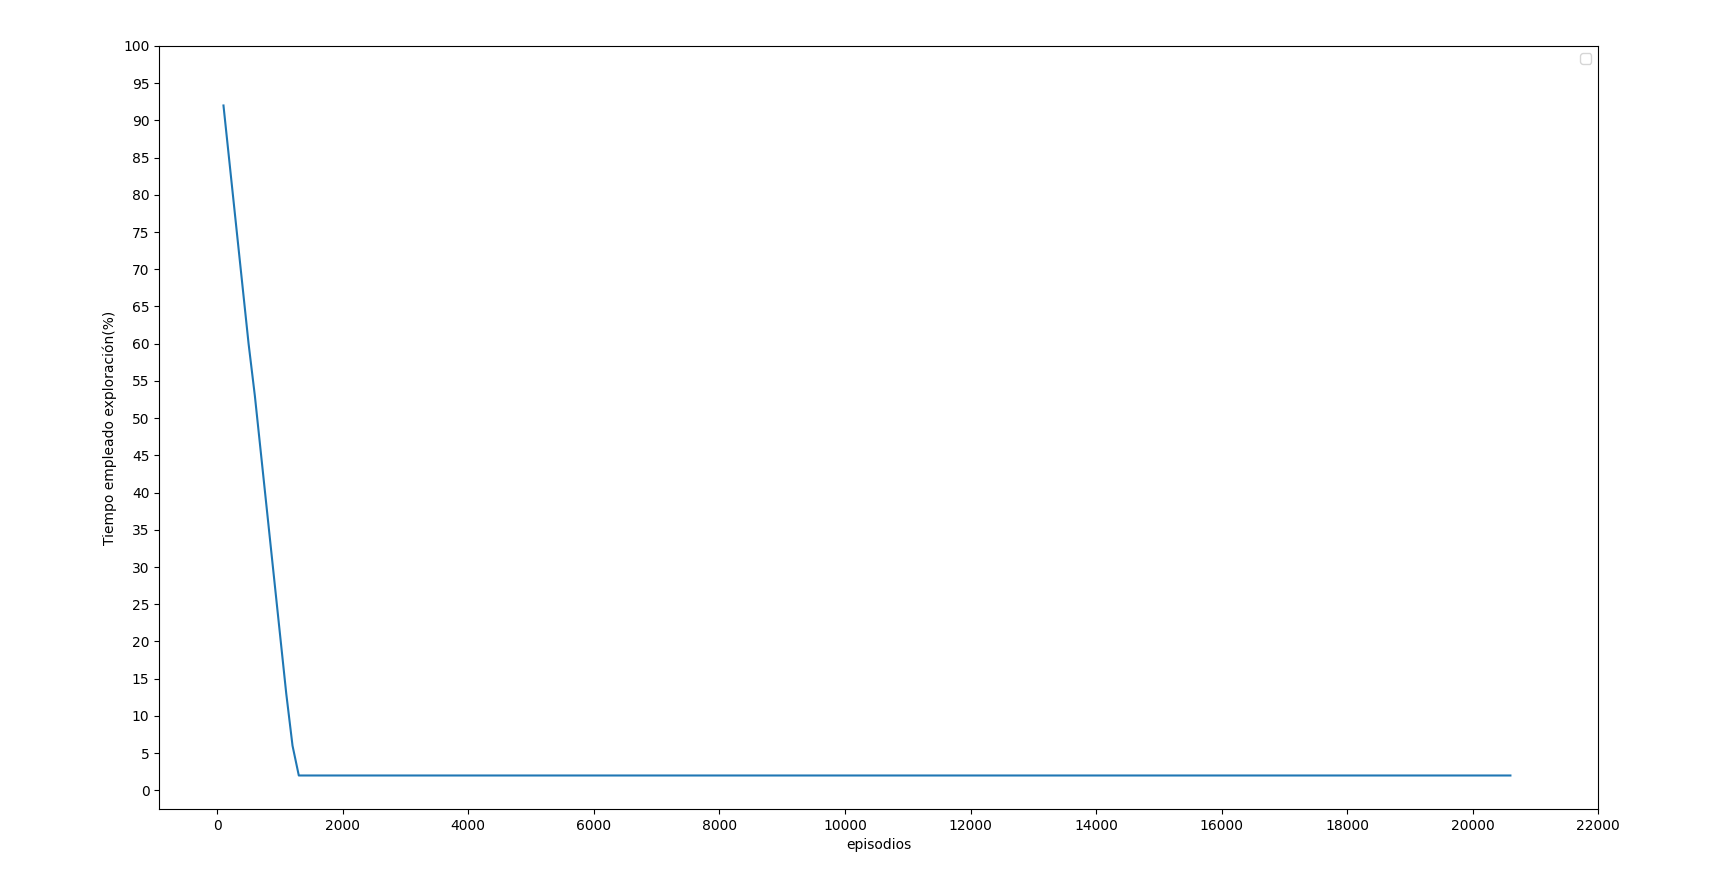
\includegraphics[scale=0.27]{mountain/mountain-dqn-time.png}
	\caption{Tiempo empleado en explorar por \textit{MountainCar} con semilla 113}
	\label{fig:mountainDQNtime} % Unique label used for referencing the figure in-text
	%\addcontentsline{toc}{figure}{Figure \ref{fig:sigmoide}} % Uncomment to add the figure to the table of contents
\end{figure} 

La mayor parte de la exploración por parte del agente se produce en los primeros 1100 episodios del entrenamiento. Empezando con un 92\% del tiempo empleado en explorar y decrece linealmente a un ritmo alto. A los 1300 episodios ya solo emplea un 2\% del tiempo en explorar, hasta el final del entrenamiento se mantiene con esa dinámica. El resto de agentes entrenados siguen este patrón de exploración con DQN. \\

Como conclusión final, los agentes suelen alcanzar su mejor media de recompensas antes de los 2000 episodios con unas recompensas de entre -110 y -140, por lo que se puede concluir que esta técnica es capaz de resolver el problema de \textit{MountainCar-v0} tal y como define el problema Gym. Aunque quizás con una reformulación de la función de recompensa los entrenamientos podrían ser más estables y predecibles. \\

El entrenamiento de la semilla 113 ha sido un caso extraordinario, alcanzando su mejores validaciones y convergencia a partir de los 5000 episodios con una recompensa de -100 y siendo capaz de mantenerse a ese nivel. Sin embargo, no es lo habitual. Si mostramos un resumen de todos los entrenamientos en una misma gráfica podemos observar la influencia de la aleatoriedad:

\begin{figure}[H]
	\centering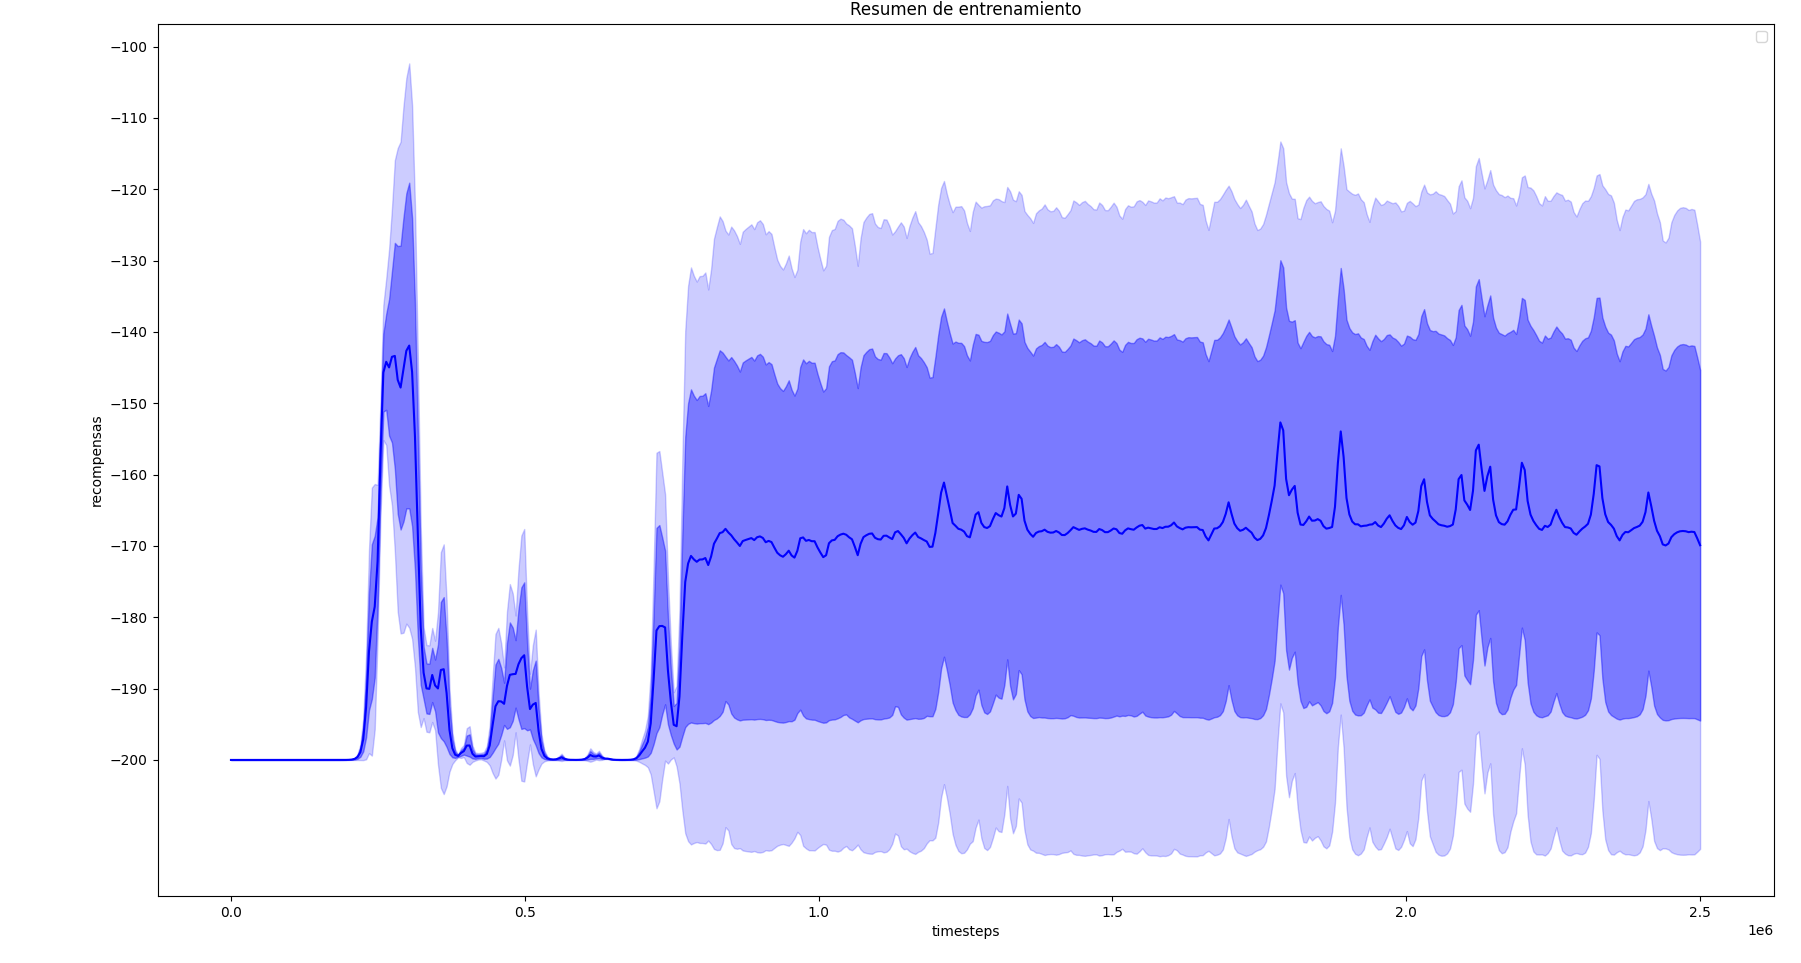
\includegraphics[scale=0.2]{mountain/mountain-dqn-media.png}
	\caption{Resumen general de progreso de algoritmo DQN en \textit{MountainCar-v0}.}
	\label{fig:mountainDQNmedia} % Unique label used for referencing the figure in-text
	%\addcontentsline{toc}{figure}{Figure \ref{fig:sigmoide}} % Uncomment to add the figure to the table of contents
\end{figure} 

Esta gráfica ha sido realizada a partir de los \textit{time-steps} dado que, como se mencionó anteriormente, si es el mismo valor en todos los modelos, cosa que no ocurre con los episodios. \\

El tono más claro muestra la desviación estándar de los datos. El tono más oscuro el error en la estimación de la media. En otras palabras, la desviación estándar dividida por la raíz cuadrada del número de semillas que tenemos. También incluye un suavizado para que la gráfica sea mejor visible. \\

La forma más simple de interpretarlo para que se entienda lo que se acaba de explicar; cuanto más estrecha sea las áreas sombreadas alrededor de la línea, más coincide el progreso en ese punto para los modelos diferentes en general. \\

Vemos la enorme variabilidad que pueden tener DQN para \textit{MountainCar-v0}, sobretodo pasados los 2000 episodios más o menos.

\subsection{DDPG}

En DDPG, se han conseguido resultados mucho más \textbf{estables} que en DQN alcanzando siempre unos resultados muy semejantes independientemente de la semilla que se usa. Por lo que, a primera vista, parece ser que no es tan dependiente de la aleatoriedad durante el aprendizaje, al menos para este problema con \textit{sparse reward}. \\

Los tiempos de ejecución para este problema son muy similares a los de DQN, quizás un poco más altos en general. Las recompensas obtenidas durante los entrenamientos han sido:

\begin{figure}[H]
	\centering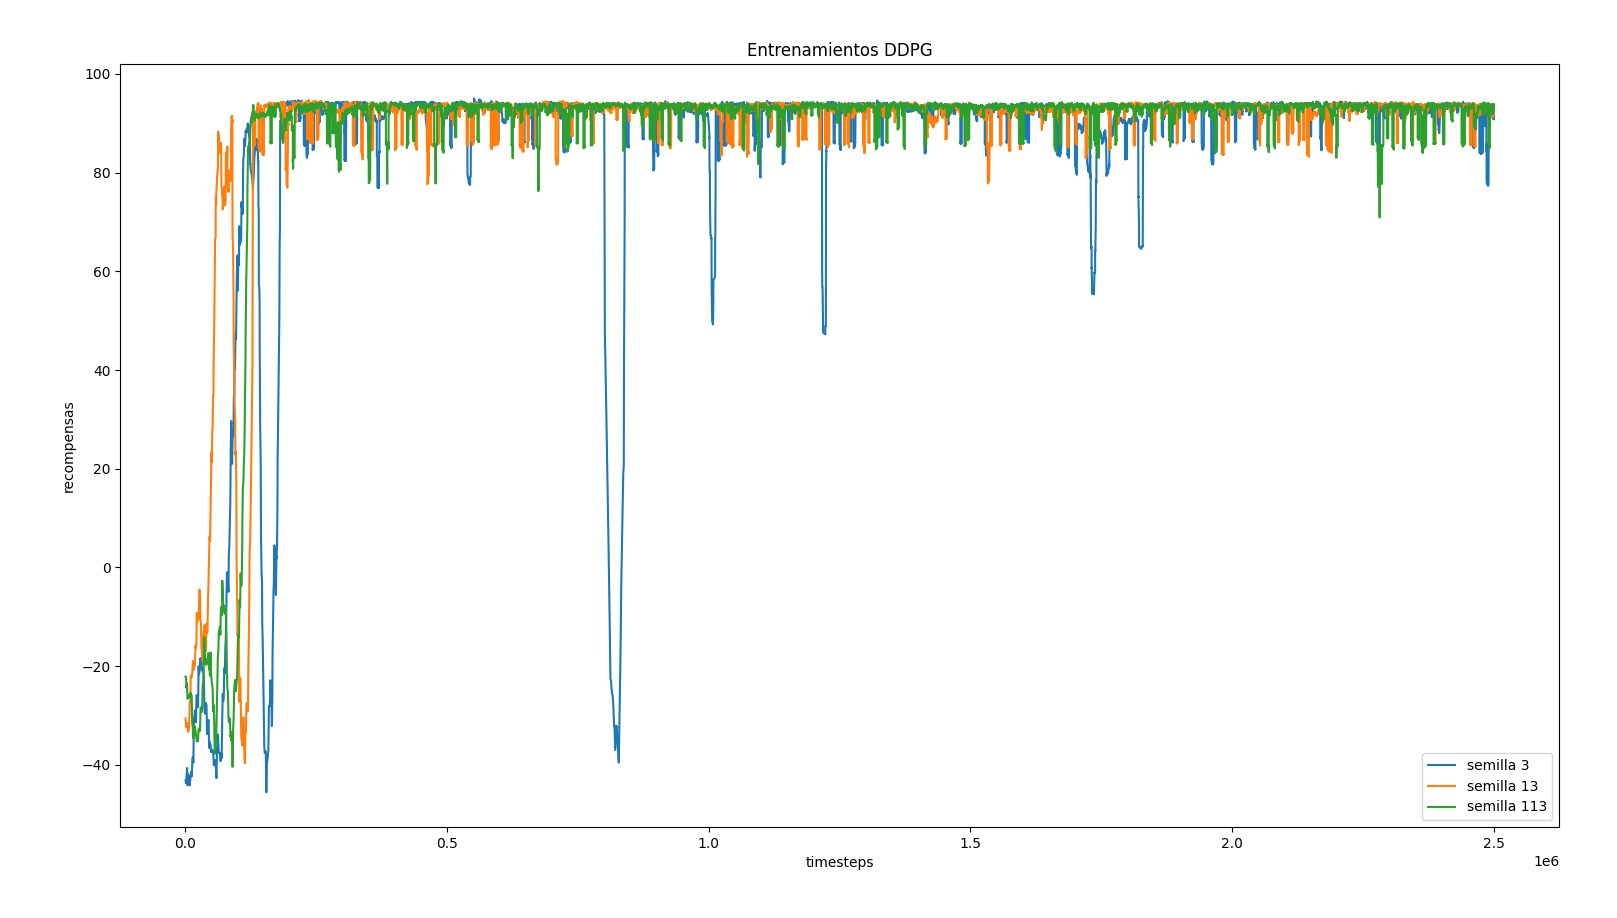
\includegraphics[scale=0.2]{mountain/mountain-ddpg.png}
	\caption{Agentes entrenados con DDPG en \textit{MountainCar-v0}.}
	\label{fig:mountainDDPG} % Unique label used for referencing the figure in-text
	%\addcontentsline{toc}{figure}{Figure \ref{fig:sigmoide}} % Uncomment to add the figure to the table of contents
\end{figure} 

Como se puede apreciar en la figura \ref{fig:mountainDDPG}, los modelos convergen bastante pronto, sobre los 200000 \textit{time-steps} de entrenamiento aproximadamente. Se mantienen muy estables, no mejoran más, pero tampoco empeoran. En la semilla 3 se produjeron algunas caídas repentinas, volviendo a sus valores habituales de recompensa rápidamente, por lo que no parece preocupante.

\begin{figure}[H]
	\centering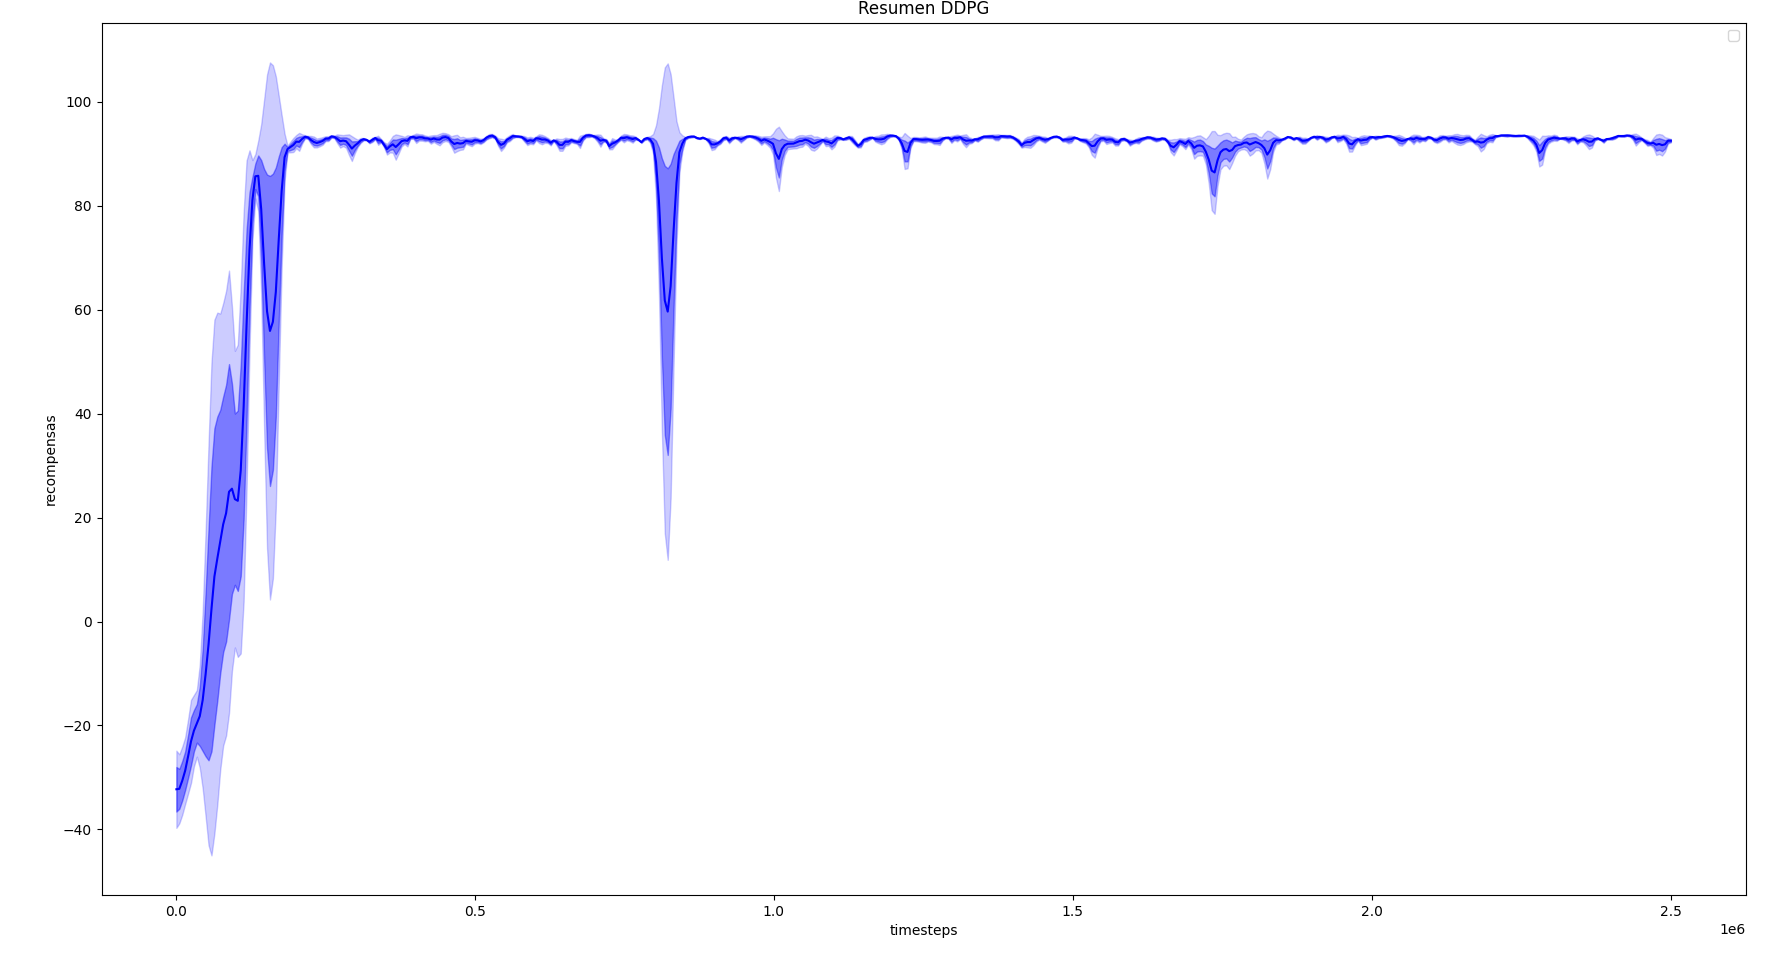
\includegraphics[scale=0.2]{mountain/mountain-ddpg-resumen.png}
	\caption{Agentes entrenados con DDPG en \textit{MountainCar-v0}.}
	\label{fig:mountainDDPGresumen} % Unique label used for referencing the figure in-text
	%\addcontentsline{toc}{figure}{Figure \ref{fig:sigmoide}} % Uncomment to add the figure to the table of contents
\end{figure}

Siguen un patrón en el progreso de aprendizaje bastante claro independientemente de la semilla que se utilice. La representación de la función de recompensa para \textit{MountainCarContinuous-v0} es diferente que para \textit{MountainCar-v0}, como ya se comentó en la sección \ref{sec:mountaincarcontinuo}. Parece que esto resuelve en gran medida el problema de \textit{sparse reward} que veíamos reflejado en DQN, a parte de que DDPG parece lidiar mejor con ello.  

\subsection{PPO2}

Lamentablemente, PPO2 no ha conseguido ningún tipo de resultados positivos. Simple y llanamente, no ha logrado alcanzar la meta ni una sola vez durante su entrenamiento, realizando episodios de duración máxima, 200 pasos. \\

¿Esto quiere decir que PPO2 es un mal algoritmo? En realidad no, es solo que no funciona para la definición de este problema. El \textit{sparse reward} hace que en este caso sea inviable para este método basado en política. \\

\subsection{Comparativa de modelos}

Si exponemos todos los resultados de modelos en una sola gráfica obtenemos lo siguiente:

\begin{figure}[H]
	\centering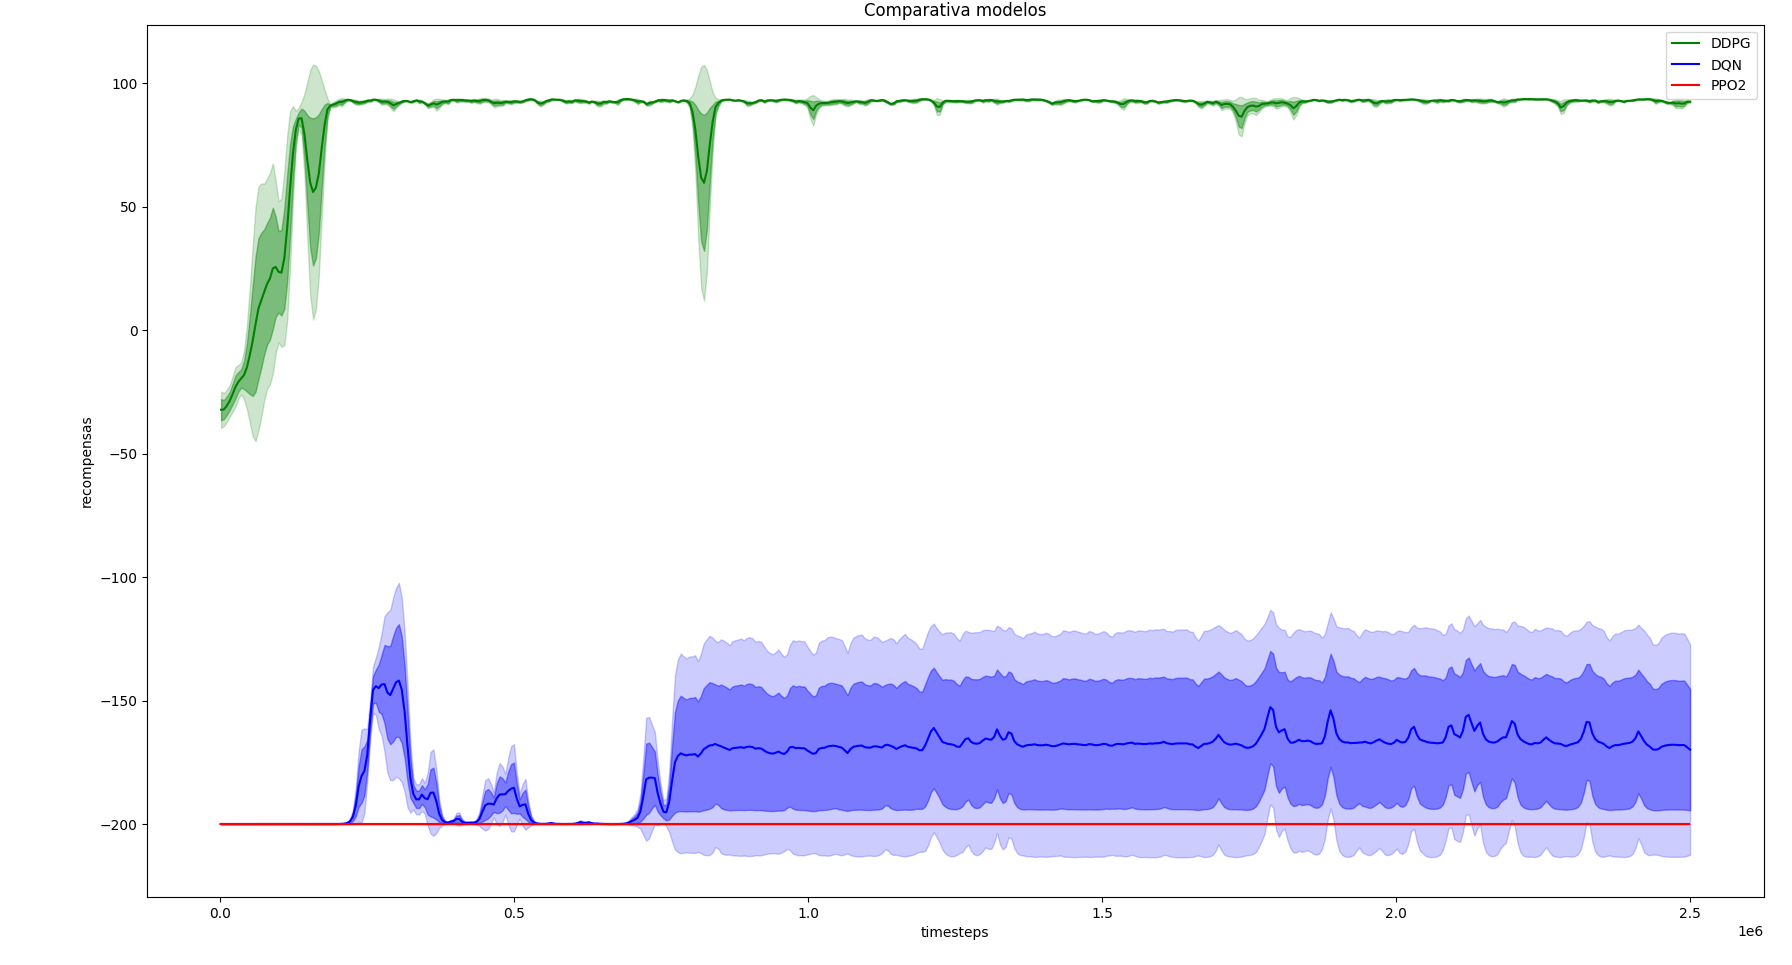
\includegraphics[scale=0.25]{mountain/resumen-mountain.png}
	\caption{Comparativa de técnicas en \textit{MountainCar}.}
	\label{fig:mountainresumen} % Unique label used for referencing the figure in-text
	%\addcontentsline{toc}{figure}{Figure \ref{fig:sigmoide}} % Uncomment to add the figure to the table of contents
\end{figure}

Hay que recordar que la escala de recompensas de \textit{MountainCarContinuous-v0} (DDPG) es diferente a la de \textit{MountainCar-v0} (DQN y PPO2). En el primer caso se entiende por un buen modelo aquel capaz de alcanzar medias de recompensas superiores a 90, en el segundo caso superiores a -110. \\

PPO2 queda descartado para la definición del porblema actual dado que no consigue ningún resultado. Aunque DQN ha demostrado poder dar buenos resultados, es demasiado dependiente de la aleatoriedad en el aprendizaje, en gran parte por el \textit{sparse reward}. Entonces, DDPG parece ser la mejor opción para las definiciones de \textit{MountainCar} actuales, por su estabilidad y superar prácticamente siempre el umbral de recompensa a partir del cual se considera un buen modelo.

\section{Super Mario Bros}

%\section{MountainCar-v0}\label{sec:exp:mountaincar}
%
%Comenzamos con el problema más sencillo que hemos utilizado (apartado \ref{sec:mountaincar}). A pesar de su simpleza, podemos entender que dependiendo del problema, y de como lo interpretamos para el agente, esto puede hacer que algunas técnicas no sean efectivas o que den resultados mejores o peores. Lo veremos a continuación. \\
%
%\subsection{DQN}\label{sec:mountain:DQN}
%
%He realizado diferentes pruebas de entrenamiento. Voy a mostrar aquellos modelos que me han parecido más interesantes. También realicé el mismo entrenamiento haciendo uso de semillas diferentes(3, 13 y 46). De esta forma, podía reentrenar el modelo en caso de que hubiera algún error y podía valorar la importancia de la aleatoriedad en cada técnica. \\
%
%\begin{figure}[H]
%	\centering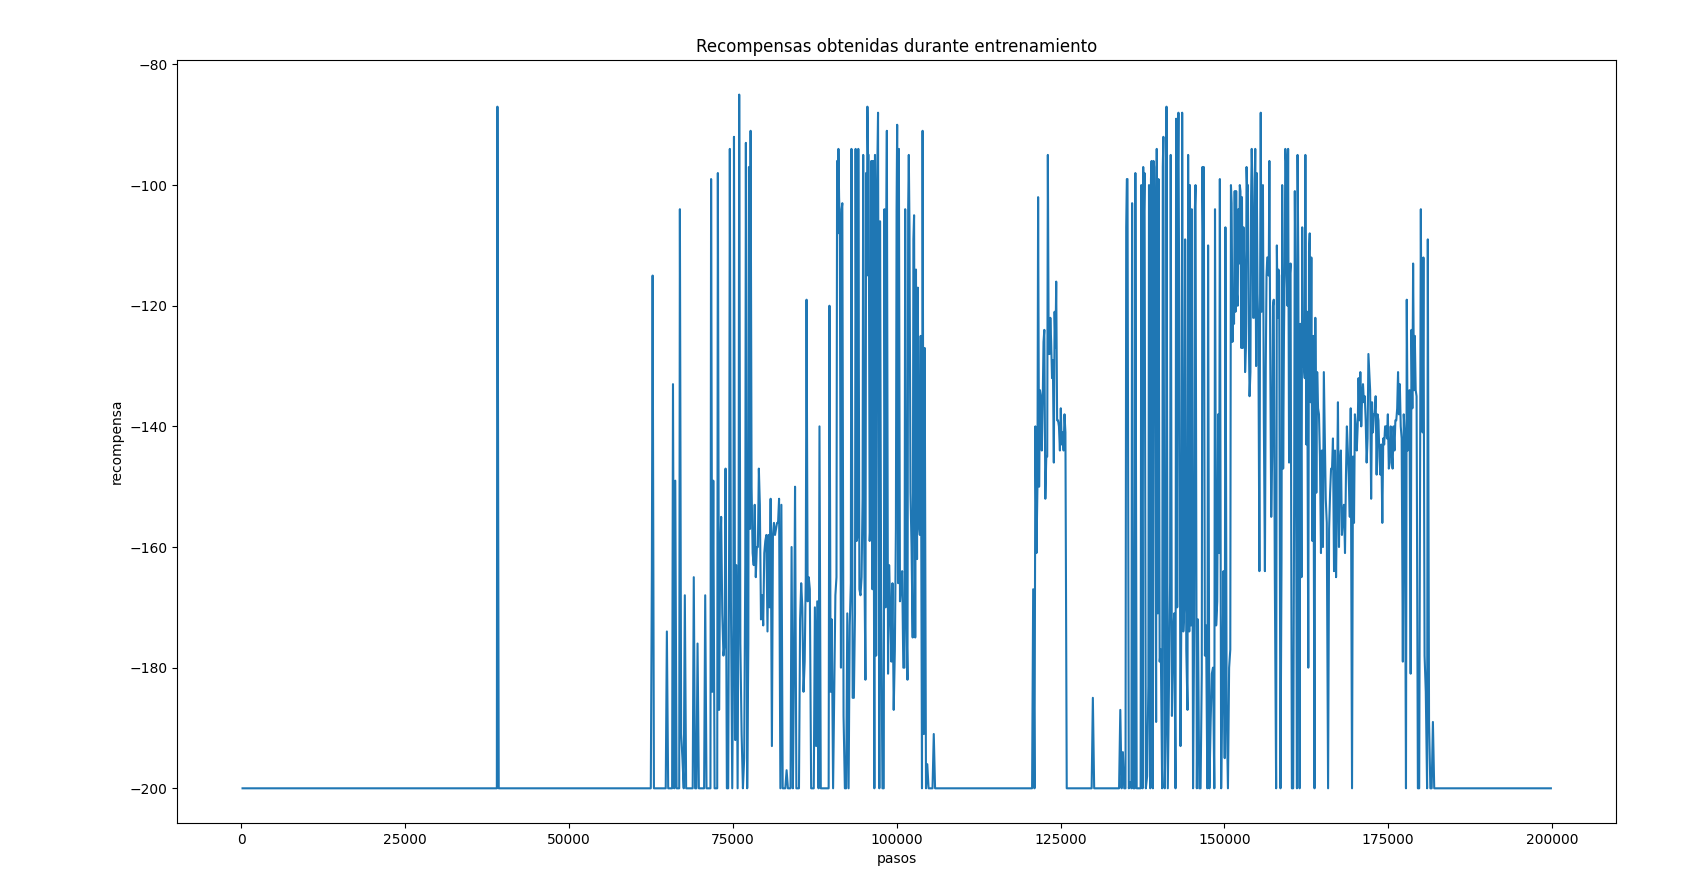
\includegraphics[scale=0.25]{mountain/DQN/3_2e5.png}
%	\caption{Gráfica de recompensas obtenidas durante entrenamiento. Algoritmo DQN, semilla 3 y en \textit{MountainCar-v0}}
%	\label{fig:mountain1} % Unique label used for referencing the figure in-text
%	%\addcontentsline{toc}{figure}{Figure \ref{fig:sigmoide}} % Uncomment to add the figure to the table of contents
%\end{figure}
%
%Esta es la primera gráfica que aprendí a generar a partir de los \textit{logs}. Con ella podemos observar las recompensas que fue obteniendo el agente en cada \textit{timestep} que realizaba de experimentación. En el caso de la figura \ref{fig:mountain1}, vemos que consiguió resolverlo tempranamente en un caso aislado, además en pocos pasos, ya que tardo unos 90 \textit{timesteps}(recompensa de -90). Lo cual quiere decir que aprovecho el momentum muy bien para conseguir subir. \\
%
%Sin embargo, por como es la gráfica, todo apunta a que fue un caso \textbf{casual}. Realmente comienza a tener más aciertos y de una forma más continua y estable posteriormente, como se puede apreciar en los picos más juntos en las otras zonas de la gráfica. Esto me hace pensar que denota un mejor entendimiento por parte del agente de como tiene que \textbf{comportarse} para conseguir su objetivo, resolverlo con \textbf{suerte} más que con conocimiento de lo que está haciendo no podemos considerarlo como éxito, aunque tampoco estoy diciendo que la primera vez lo resuelva de forma 100\% aleatoria ya que es prácticamente imposible.
%
%\begin{figure}[H]
%	\centering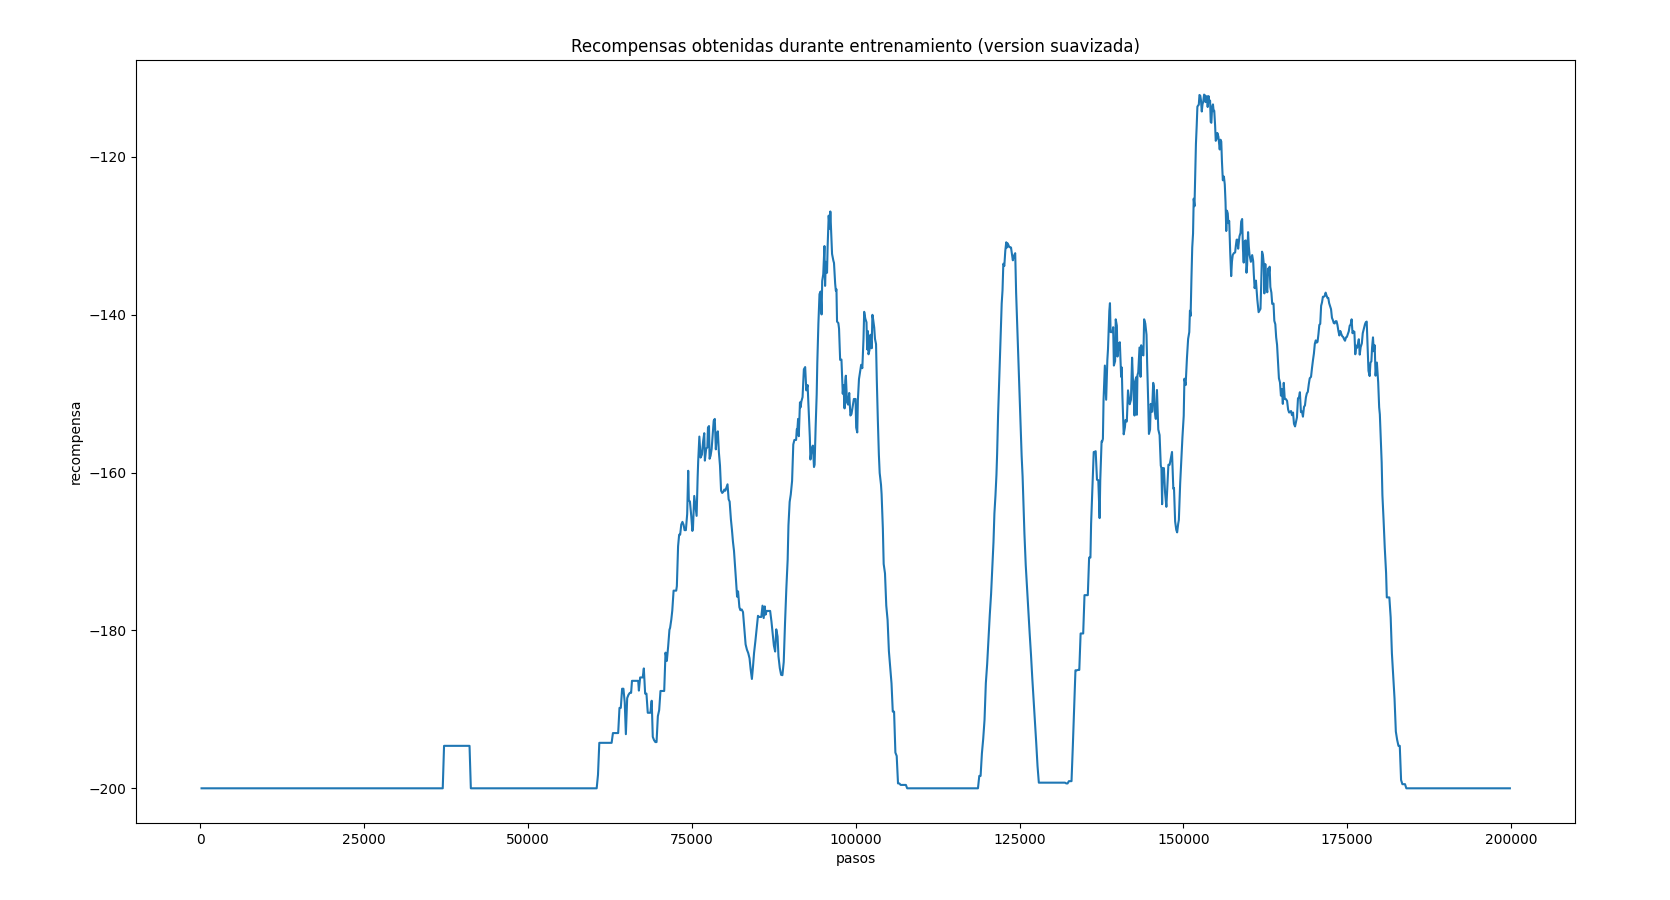
\includegraphics[scale=0.25]{mountain/DQN/3_2e5_suave.png}
%	\caption{Recompensas obtenidas durante entrenamiento(versión suavizada de la figura \ref{fig:mountain1}). Algoritmo DQN, semilla 3 y en \textit{MountainCar-v0}}
%	\label{fig:mountain2} % Unique label used for referencing the figure in-text
%	%\addcontentsline{toc}{figure}{Figure \ref{fig:sigmoide}} % Uncomment to add the figure to the table of contents
%\end{figure}
%
%El siguiente objetivo que busqué fue el tratar, de alguna manera, de suavizar aquellas subidas que no estaban tan motivadas por un buen conocimiento. Por ello, construimos una gráfica a partir de la anterior, solo que \textbf{suavizada}. Cada punto tiene un valor que depende de los valores que tiene alrededor, son influidos por sus vecinos. \\
%
%El resultado es la figura \ref{fig:mountain1}. Fijémonos en el primer éxito que tiene. Ahora la subida en la recompensa es muy pequeña en comparación de las que hay más adelante, justo lo que sospechábamos. \\
%
%Podemos ir más allá. En lugar de utilizar un suavizado de los datos de las recompensas, utilizar directamente las medias obtenidas por episodios, de los cuales hablamos en el apartado \ref{sec:logs}
%
%\begin{figure}[H]
%	\centering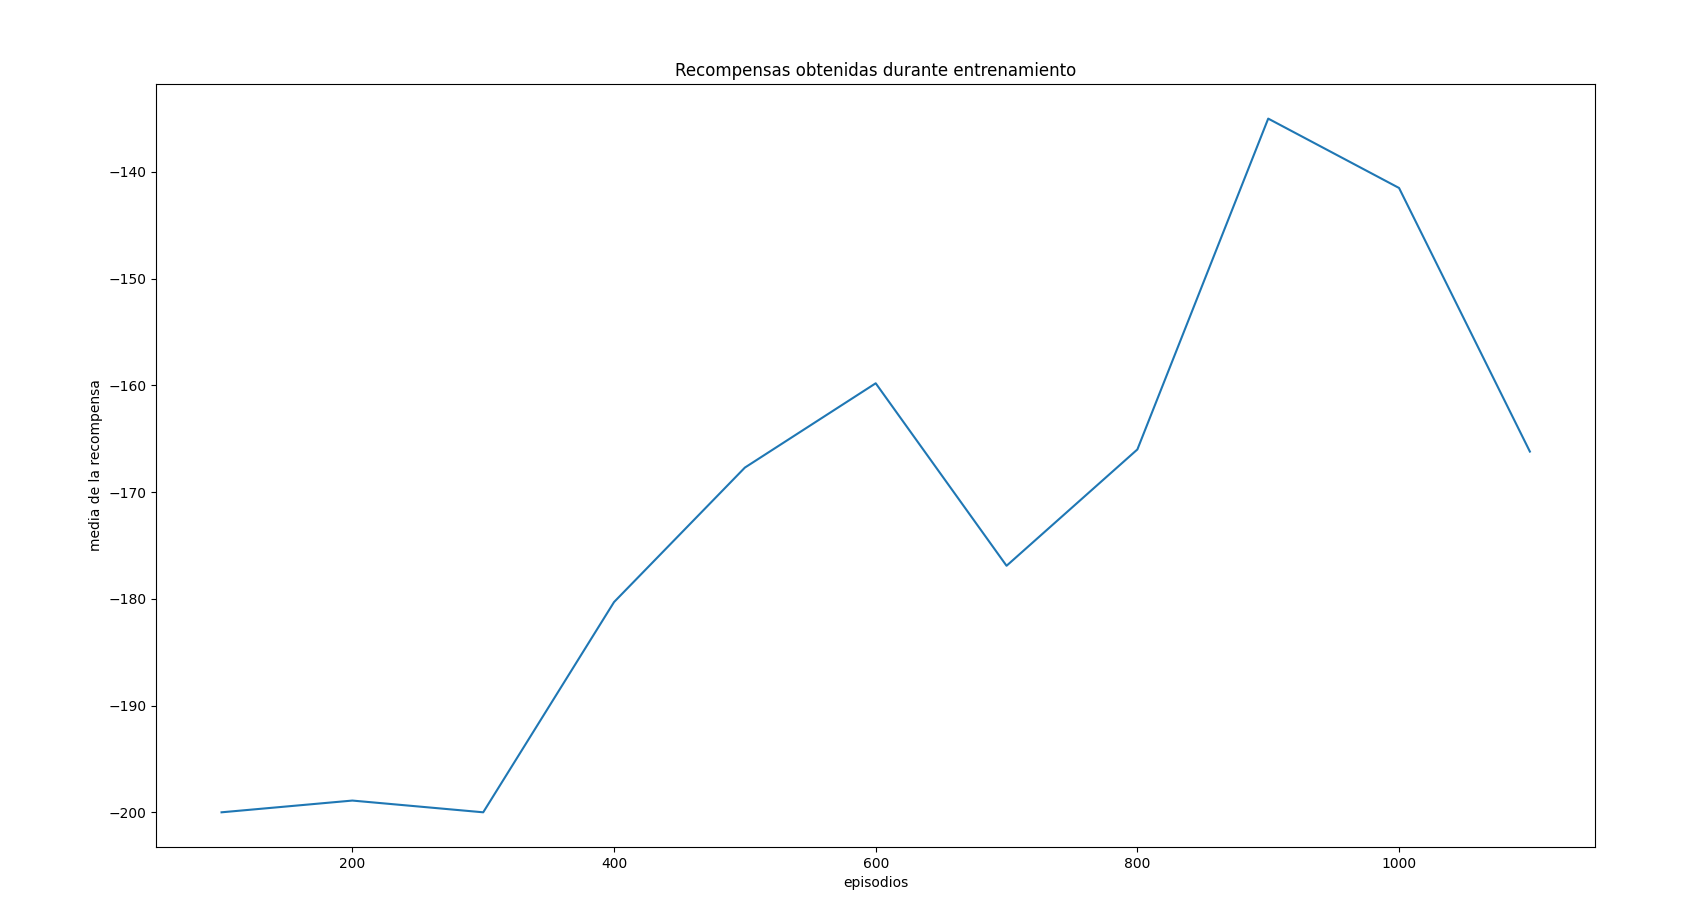
\includegraphics[scale=0.25]{mountain/DQN/3_2e5_resumen.png}
%	\caption{Media de recompensas obtenidas cada 100 episodios. Algoritmo DQN, semilla 3 y en \textit{MountainCar-v0}.}
%	\label{fig:mountain3} % Unique label used for referencing the figure in-text
%	%\addcontentsline{toc}{figure}{Figure \ref{fig:sigmoide}} % Uncomment to add the figure to the table of contents
%\end{figure}
%
%La figura \ref{fig:mountain3}, tiene el mismo objetivo que lo explicado anteriormente, dar más valor a aquellos éxitos que son resultado de un aprendizaje real y menos de la aleatoriedad, solo que aún más extremo. \\
%
%Vemos que ahora la primera subida apenas es apreciable directamente, sin embargo, las otras dos zonas que tenía muchos éxitos son aún mas escarpadas. Como resumen de estas pruebas para la semilla 3 en DQN y \textit{MountainCar-v0}, llegamos a la conclusión de que durante el entrenamiento pasa por \textbf{dos etapas}. Hay una primera subida general de los resultados, que luego se desploma, seguramente porque no consigue actualizarse correctamente a partir de esos éxitos y se actualiza a una versión peor de sí mismo. No obstante, luego es capaz de recuperarse cuando vuelve a comenzar a fallar y consigue resultados aún mejores. Por último, comienza otro desplome de su comportamiento, por suerte el algoritmo hace actualizaciones del modelo siempre que se considera que mejora y se va quedando guardada la \textbf{última mejor versión} registrada. \\
%
%Hice las mismas pruebas para las semillas 13 y 46, muestro las gráficas a continuación:
%
%\begin{figure}[H]
%	\centering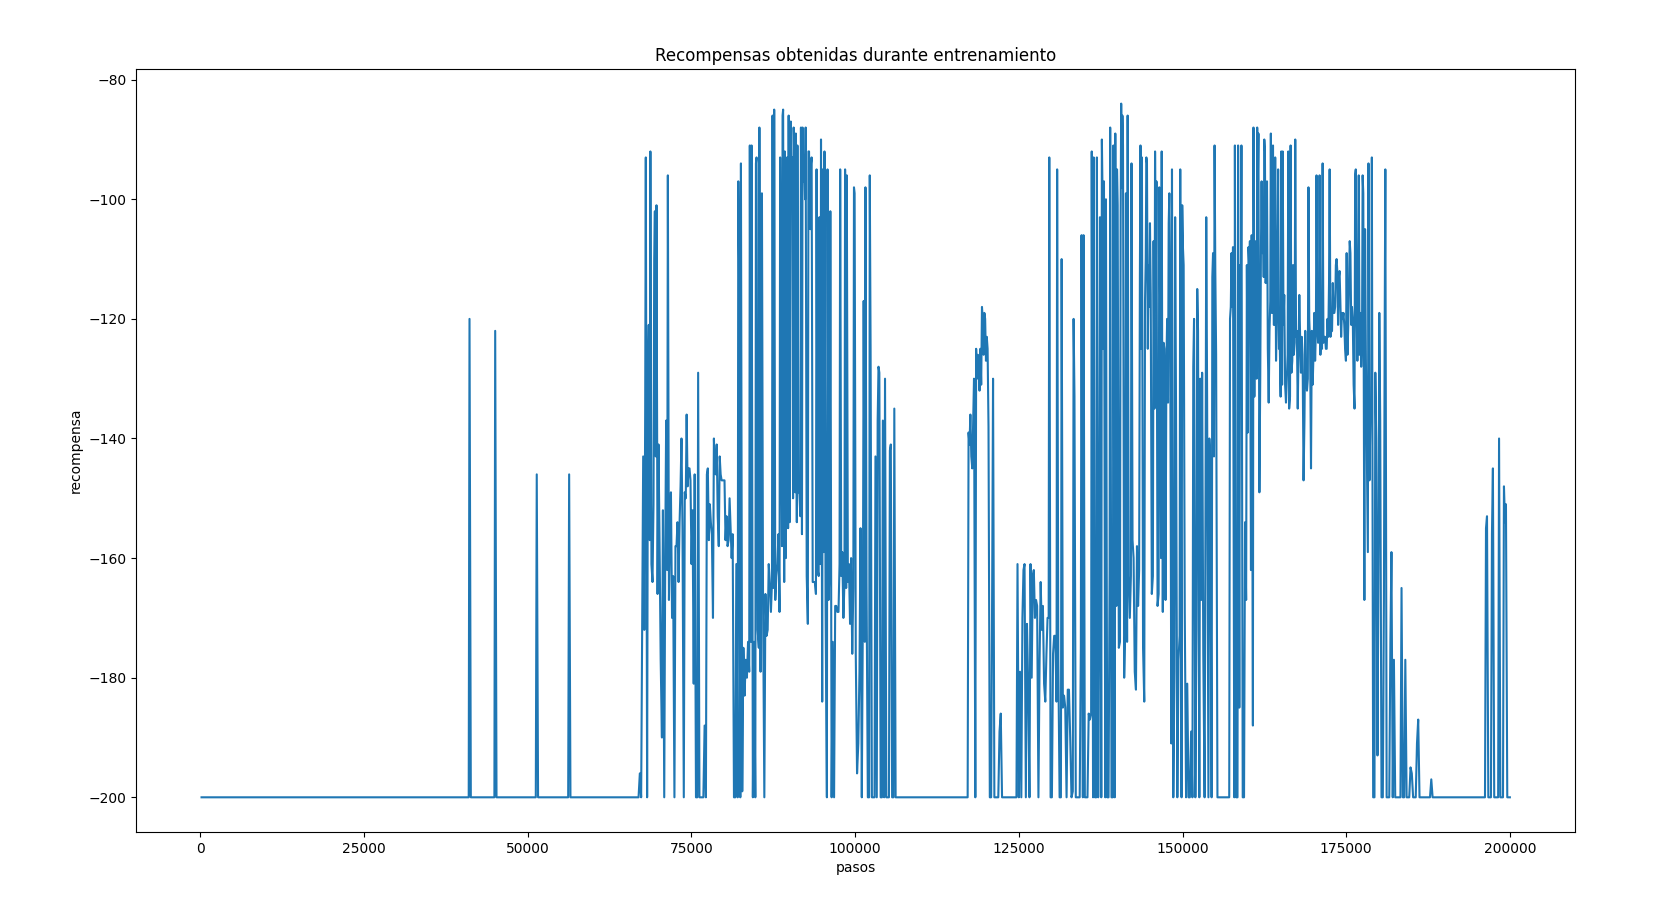
\includegraphics[scale=0.25]{mountain/DQN/13_2e5.png}
%	\caption{Gráfica de recompensas obtenidas durante entrenamiento. Algoritmo DQN, semilla 13 y en \textit{MountainCar-v0}.}
%	\label{fig:mountain4} % Unique label used for referencing the figure in-text
%	%\addcontentsline{toc}{figure}{Figure \ref{fig:sigmoide}} % Uncomment to add the figure to the table of contents
%\end{figure}
%
%
%\begin{figure}[H]
%	\centering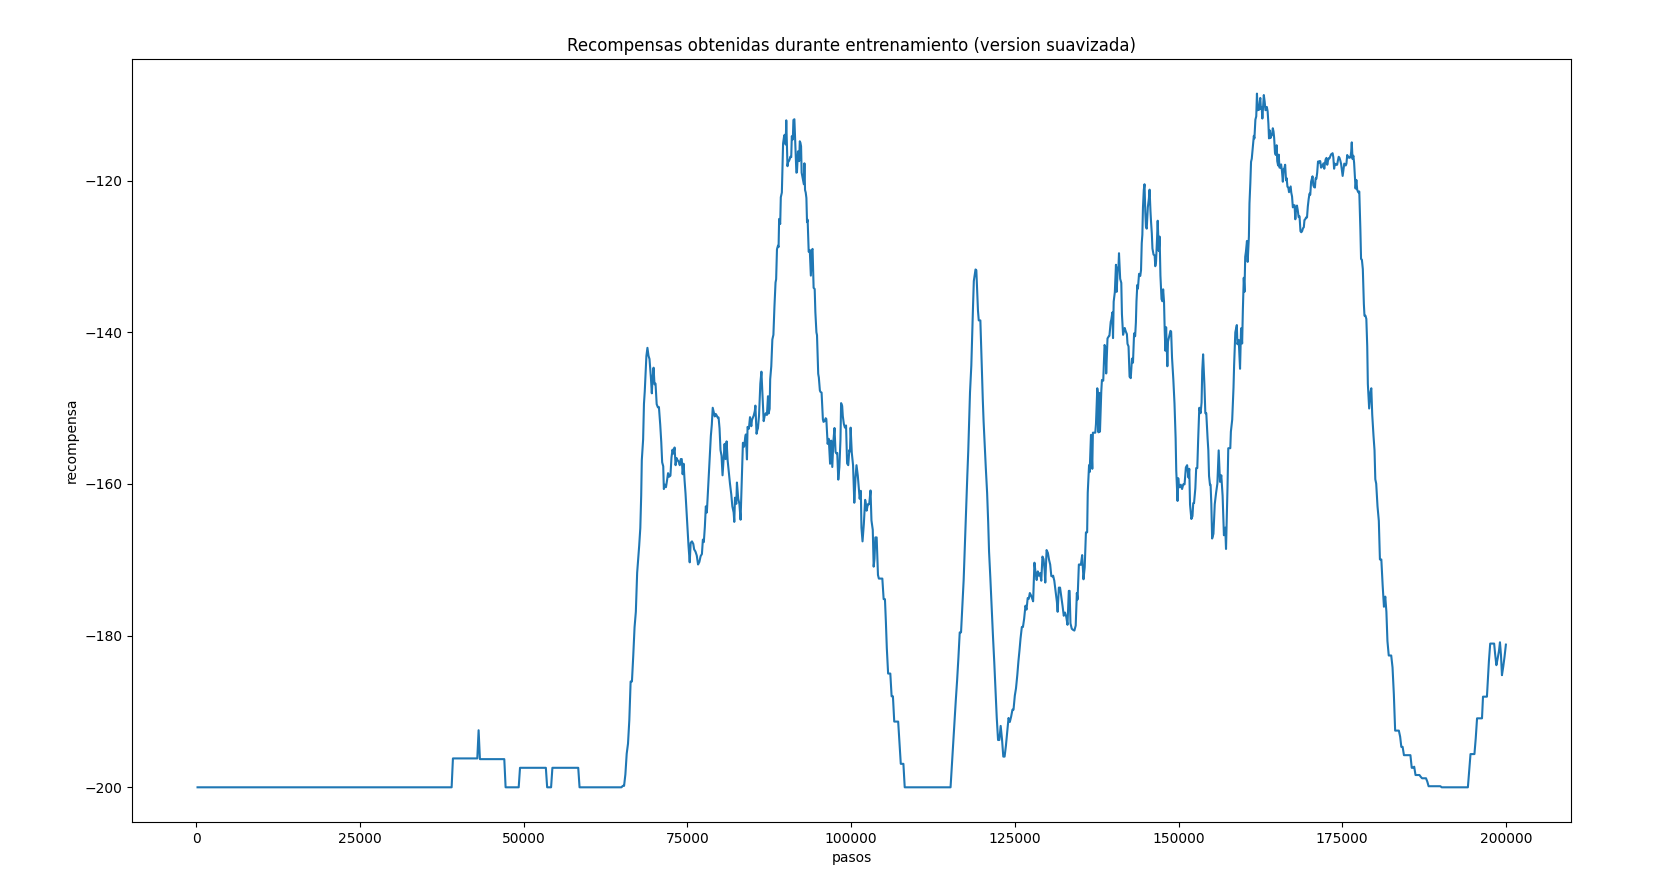
\includegraphics[scale=0.25]{mountain/DQN/13_2e5_suave.png}
%	\caption{Recompensas obtenidas durante entrenamiento(versión suavizada de la figura \ref{fig:mountain4}). Algoritmo DQN, semilla 13 y en \textit{MountainCar-v0}.}
%	\label{fig:mountain5} % Unique label used for referencing the figure in-text
%	%\addcontentsline{toc}{figure}{Figure \ref{fig:sigmoide}} % Uncomment to add the figure to the table of contents
%\end{figure}
%
%\begin{figure}[H]
%	\centering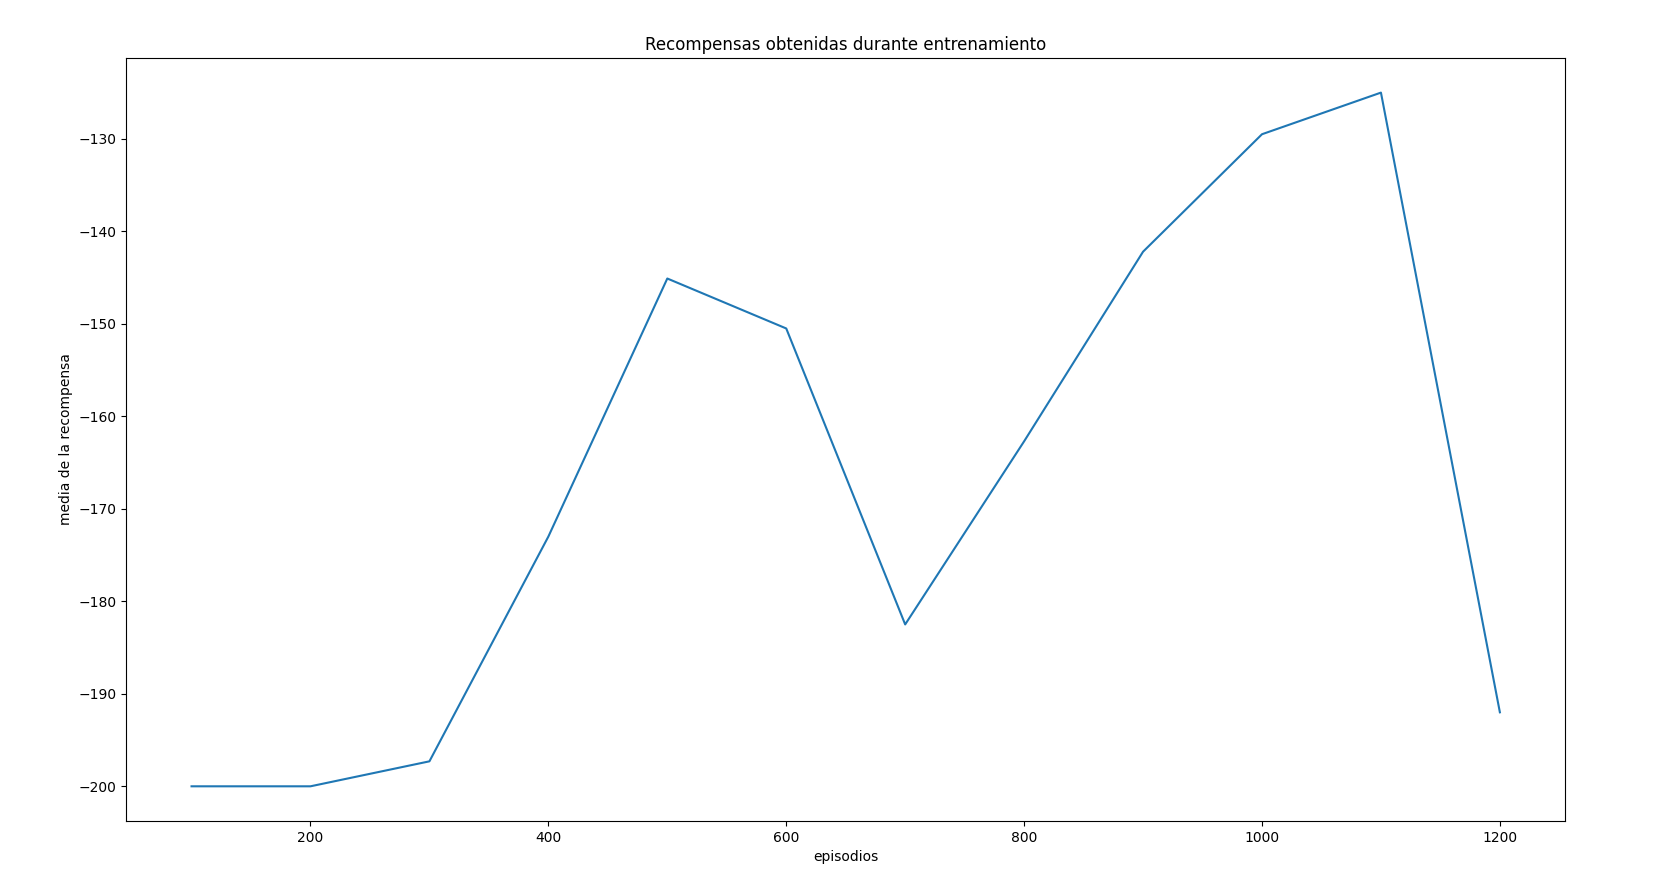
\includegraphics[scale=0.25]{mountain/DQN/13_2e5_resumen.png}
%	\caption{Media de recompensas obtenidas cada 100 episodios. Algoritmo DQN, semilla 13 y en \textit{MountainCar-v0}.}
%	\label{fig:mountain6} % Unique label used for referencing the figure in-text
%	%\addcontentsline{toc}{figure}{Figure \ref{fig:sigmoide}} % Uncomment to add the figure to the table of contents
%\end{figure}
%
%\begin{figure}[H]
%	\centering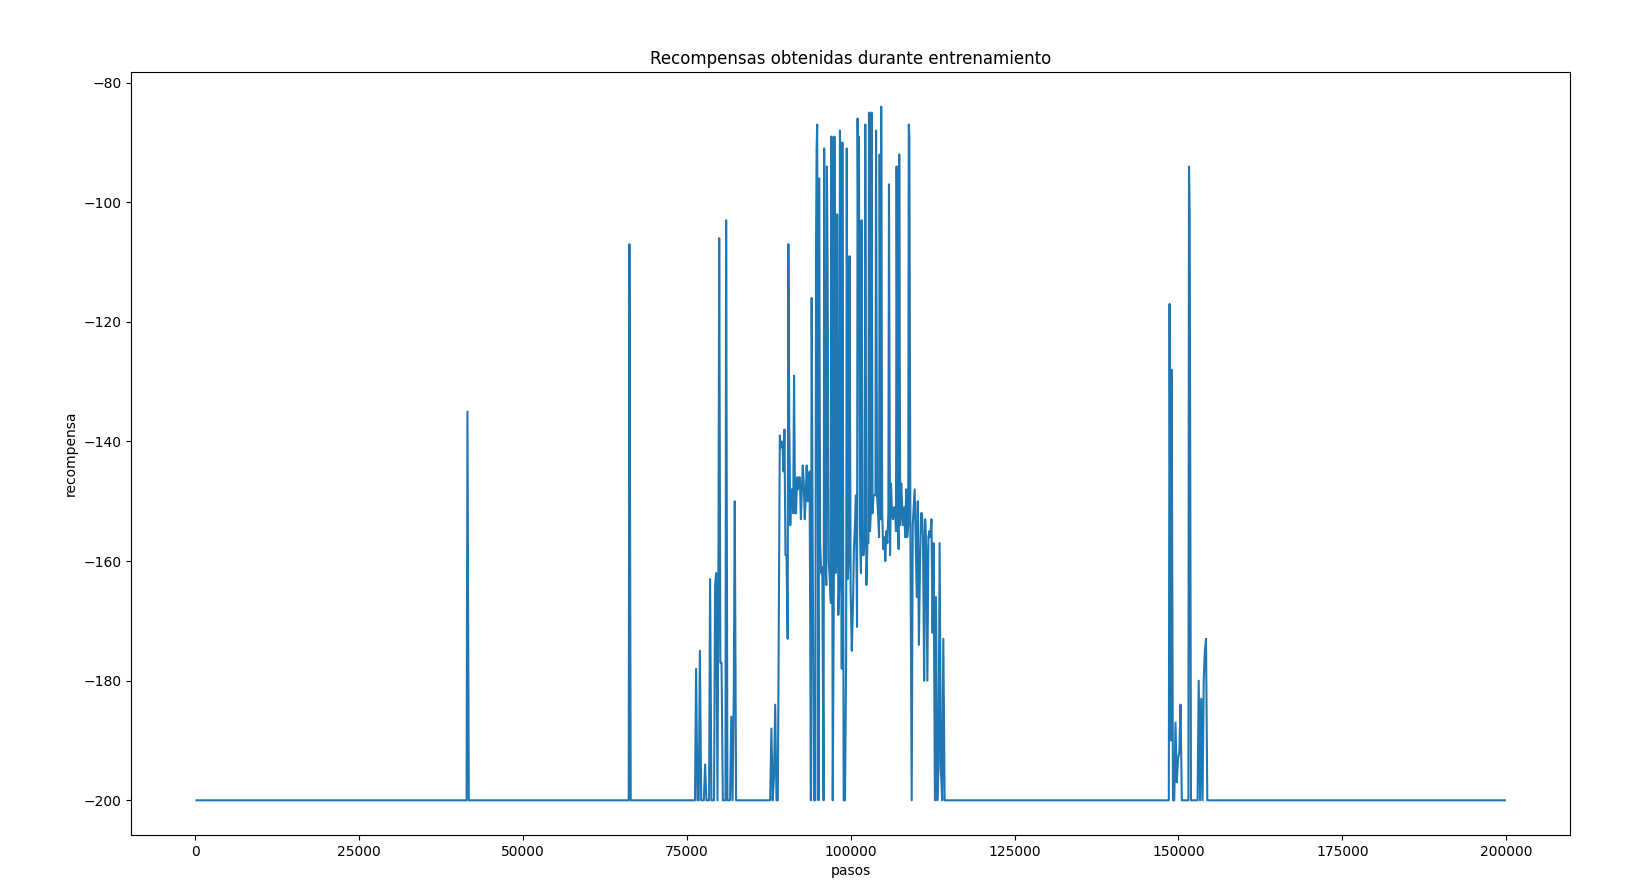
\includegraphics[scale=0.25]{mountain/DQN/46_2e5.png}
%	\caption{Gráfica de recompensas obtenidas durante entrenamiento. Algoritmo DQN, semilla 46 y en \textit{MountainCar-v0}.}
%	\label{fig:mountain7} % Unique label used for referencing the figure in-text
%	%\addcontentsline{toc}{figure}{Figure \ref{fig:sigmoide}} % Uncomment to add the figure to the table of contents
%\end{figure}
%
%\begin{figure}[H]
%	\centering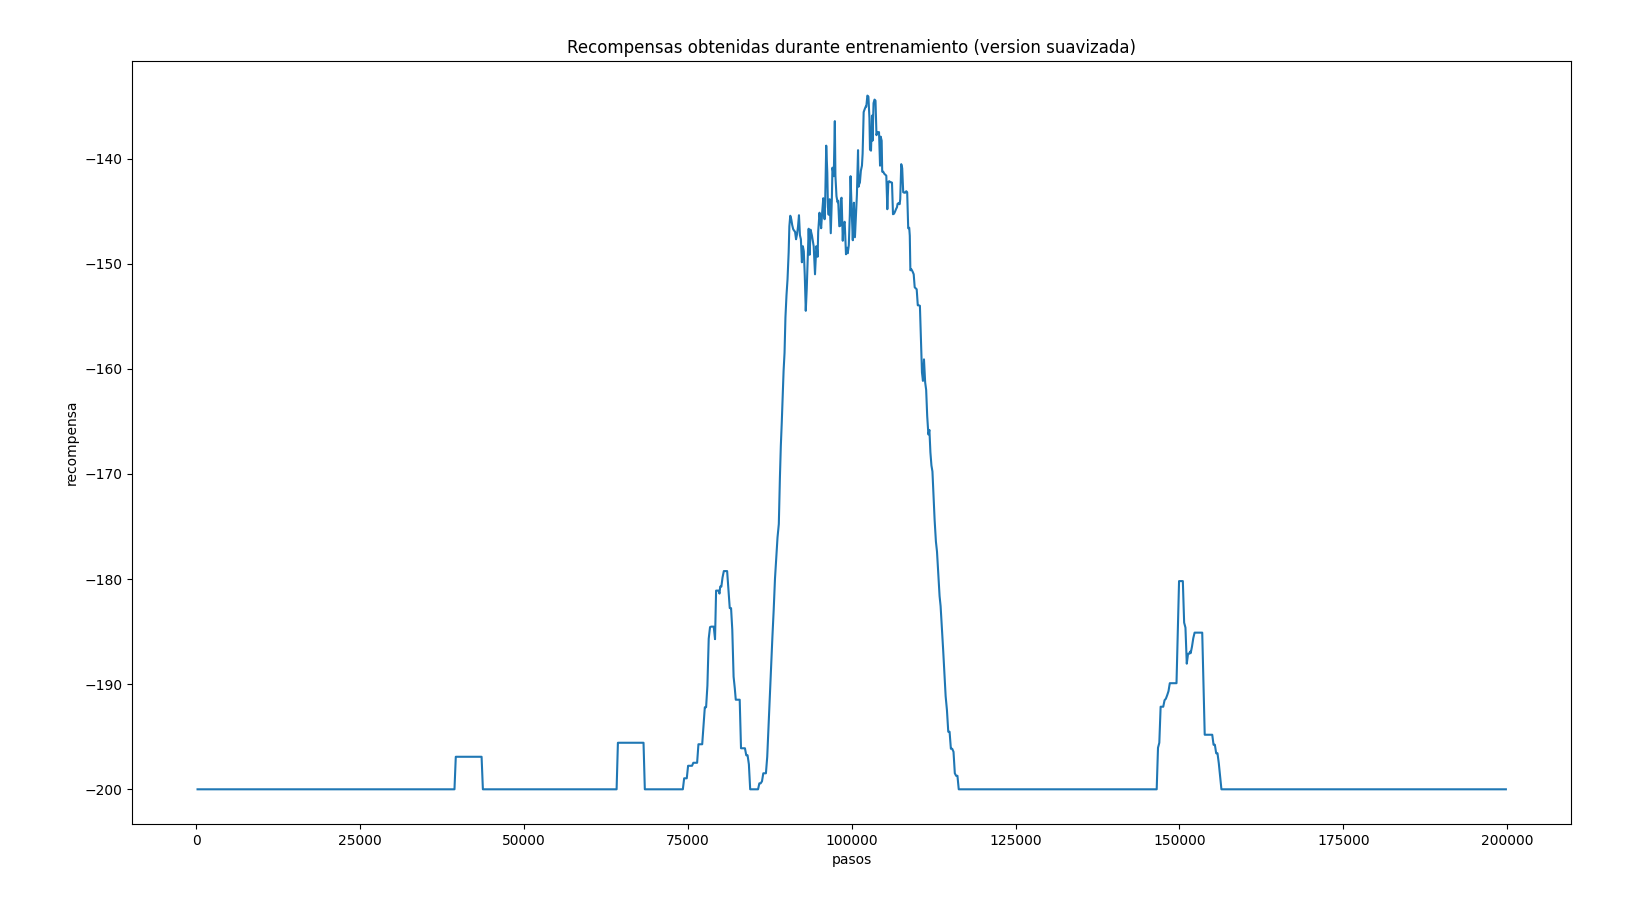
\includegraphics[scale=0.25]{mountain/DQN/46_2e5_suave.png}
%	\caption{Recompensas obtenidas durante entrenamiento(versión suavizada de la figura \ref{fig:mountain7}). Algoritmo DQN, semilla 46 y en \textit{MountainCar-v0}.}
%	\label{fig:mountain8} % Unique label used for referencing the figure in-text
%	%\addcontentsline{toc}{figure}{Figure \ref{fig:sigmoide}} % Uncomment to add the figure to the table of contents
%\end{figure}
%
%\begin{figure}[H]
%	\centering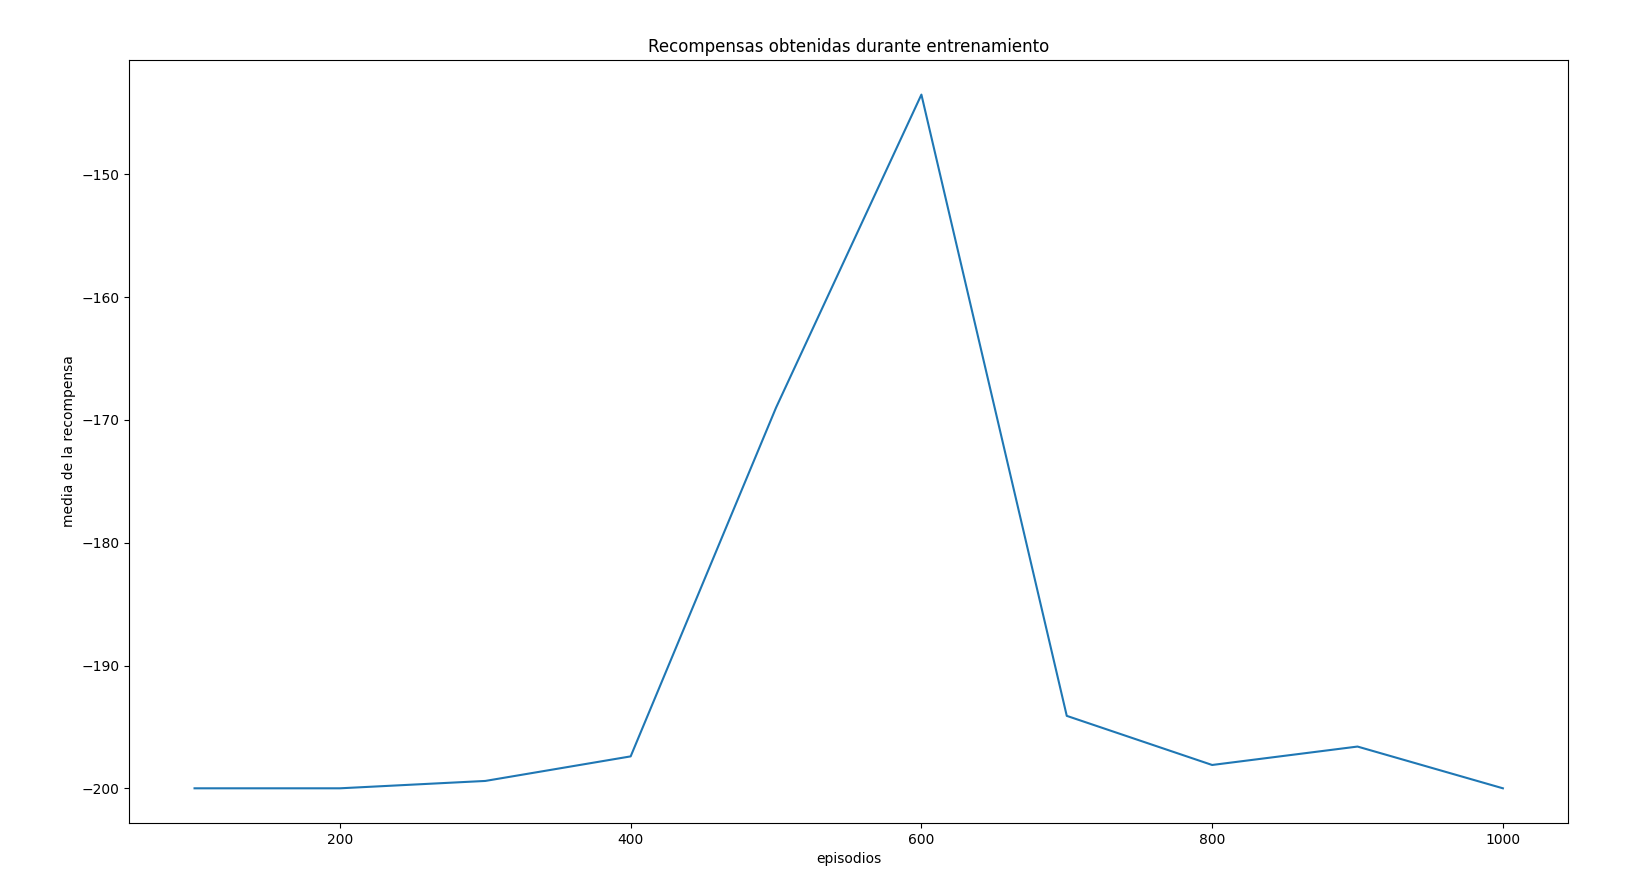
\includegraphics[scale=0.25]{mountain/DQN/46_2e5_resumen.png}
%	\caption{Media de recompensas obtenidas cada 100 episodios. Algoritmo DQN, semilla 46 y en \textit{MountainCar-v0}.}
%	\label{fig:mountain9} % Unique label used for referencing the figure in-text
%	%\addcontentsline{toc}{figure}{Figure \ref{fig:sigmoide}} % Uncomment to add the figure to the table of contents
%\end{figure}
%
%Vemos que en la semilla 13 tiene una \textbf{estructura similar}, mientras que la semilla 46 solo tiene una subida significativa más o menos a mitad del entrenamiento. \\
%
%Cuando vi los resultados llegué a la siguiente conclusión: nos encontramos ante un problema sencillo, el cual no tiene muchas posibilidades a nivel de acciones para que el agente pueda realizar. Una vez es bueno en su entorno, con las siguientes actualizaciones es mucho más \textbf{probable que empeore} a que mejore. En este caso, solo hay una forma de hacer las cosas bien para llevar la carreta a su meta, una vez aprendida, la exploración solo va a dar resultados negativos. \\
%
%Por esa misma razón pienso que se suceden estos ciclos de subida y bajada en las recompensas. Es capaz de aprender de sus errores, pero una vez comienza a acertar no es capaz de aprender de sus éxitos de una forma tan buena. Hago hincapié en que no es preocupante, ya que siempre se guarda el modelo del mejor agente durante todo el entrenamiento, no el que queda cuando termina. \\
%
%También podemos llegar a pensar; si estos algoritmos son capaces de reforzar las buenas acciones para que las repita en situaciones similares, ¿por qué en este caso no es así? Otras de las conclusiones que he sacado a partir de estos experimentos, es que considero que el sistema de \textbf{recompensas} que utiliza OpenAI para este entorno \textbf{no es óptimo} para esta técnica. \\
%
%En el apartado \ref{sec:mountaincar} mencionamos que la recompensa de este entorno es siempre -1 a no ser que alcance la meta, en ese paso el valor de la recompensa es 1. Creo que este sistema no ayuda al agente de ninguna manera a determinar si sus acciones son buenas o no y solo se puede dejar llevar por el resultado final para aprender. Entonces, el agente no puede diferenciar entre buenas y malas acciones. En su lugar, refuerza todas las acciones que ha realizado cuando tiene éxito, aunque dentro tenga decisiones malas y quita relevancia a todas las decisiones tomadas durante un fracaso, aunque en ese intento haya tomado algunas buenas decisiones en realidad. \\
%
%Estaría bien que la recompensa fuera positiva cuando se detectase que la carreta está aprovechando el momentum para subir, y negativa en caso sontrario. No osbtante, no siempre vamos a saber la mejor manera de resolver los problemas para un entorno dado, y menos cuando son mucho más complejos que éste. \\
%
%Entonces, en el momento que comienza a tener éxito, sigue explorando un 2\% de su tiempo como veremos a continuación. Como el problema es muy sencillo y solo hay una manera de hacerlo bien, ese 2\% de exploración puede hacer que el agente erre en su intento y, como consecuencia, desfavorezca al resto de deciones buenas que ya había aprendido a tomar. \\
%
%
%Creo que es un ejemplo magnífico para entender la gran \textbf{importancia} en la \textbf{definición del problema} que se trata de resolver. dependiendo de esa definición, no solo la representación de la recompensa, sino el formato de input, output y ventajas, en caso de utilizarlas, puede hacer que una técnica consiga funcionar mejor o peor al procesar la experiencia que recoge. Es como elegir la mejor función de pérdida para una red neuronal, esa decisión puede cambiarlo todo.
%
%
%
%\begin{figure}[H]
%	\centering\includegraphics[scale=0.25]{mountain/DQN/46_2e5_time.png}
%	\caption{Porcentaje de tiempo empleado en explorar para algoritmo DQN en \textit{MountainCar-v0}.}
%	\label{fig:mountain10} % Unique label used for referencing the figure in-text
%	%\addcontentsline{toc}{figure}{Figure \ref{fig:sigmoide}} % Uncomment to add the figure to the table of contents
%\end{figure}
%
%En la figura \ref{fig:mountain10} vemos el porcentaje de tiempo empleado por el agente para explorar. Como ya hemos mencionado, no es mucho debido a la simplicidad del entorno y que explorar otras alternativas a las que el agente piensa no va a ser bueno. Sería interesante incluso implementar un sistema que redujera ese porcentaje a 0 cuando se superara una cierta recompensa. Estoy convencido de que esto mejoraría aún más los resultados o, al menos, estabilizaría más el aprendizaje. Por desgracia, no he tenido el suficiente tiempo para hacerlo. \\
%
%¿Hasta que punto influye la aleatoriedad en el progreso de su aprendizaje con esta técnica? Por esta cuestión es por a que he ejecutado la misma técnica con semillas diferentes. Podemos hacer una gráfica que resuma todos los datos que hemos visto anteriormente en una sola. Mezclando los tres modelos diferentes y plasmarlos como uno solo:
%
%\begin{figure}[H]
%	\centering\includegraphics[scale=0.25]{mountain/DQN/general.png}
%	\caption{Resumen general de progreso de algoritmo DQN en \textit{MountainCar-v0}.}
%	\label{fig:mountain11} % Unique label used for referencing the figure in-text
%	%\addcontentsline{toc}{figure}{Figure \ref{fig:sigmoide}} % Uncomment to add the figure to the table of contents
%\end{figure}
%
%El tono más claro muestra la desviación estándar de los datos. El tono más oscuro el error en la estimación de la media. En otras palabras, la desviación estándar dividida por la raíz cuadrada del número de semillas que tenemos. También incluye un suavizado para que la gráfica sea más estable. \\
%
%La forma más simple de interpretarlo para que se entienda lo que acabo de explicar; cuanto más estrecha sea las áreas sombreadas alrededor de la línea, más coincide el progreso en ese punto para los tres modelos diferentes que hemos visto. \\
%
%Entonces, tenemos zonas más relevantes en la gráfica de la figura \ref{fig:mountain11}. Al principio coincide de forma perfecta que los tres modelos no son capaces de cumplir su objetivo, luego comienzan a tener algunos éxitos puntuales. La primera mejora sustancial de los datos es bastante común en el mismo punto del aprendizaje y después es un poco más variable de la aleatoriedad. Sin embargo, al final, hay una gran coincidencia de nuevo; todos empeoran hasta no ser capaces ni siquiera de cumplir el objetivo de alcanzar la meta y luego comienzan a remontar, pero aquí se acaba la gráfica. Esto me hace pensar que las conclusiones expresadas anteriormente son bastante firmes en cuanto a tiempo, sucediéndose en momentos similares en tres casos distintos.\\
%
%Como conclusión, diría que esta gráfica es muy útil para saber qué puntos del aprendizaje, como la primera mejora real de resultados o el empeoramiento final, no son dependientes del azar, sino que vienen muy determinados directamente por el algoritmo y el entorno. Por otro lado, también nos ayuda a entender qué partes del entrenamiento son más influenciables por el azar, como hemos podido observar.
%
%\subsection{PPO2}\label{sec:mountain:PPO2}
%
%Con esta técnica para este entorno no tenemos mucho que decir, por desgracia. Los resultados obtenidos fueron un completo \textbf{fracaso}. Por alguna razón, no consiguió siquiera resolver el problema que se le planteaba ni una sola vez. Se probó a quintuplicar la cantidad de \textit{timesteps} de entrenamiento (hasta el millón), no hubo ningún cambio.
%
%\begin{figure}[H]
%	\centering\includegraphics[scale=0.25]{mountain/PPO2/PPO2_fallo.png}
%	\caption{Recompensa obtenida con el algoritmo PPO2 en \textit{MountainCar-v0}, independientemente de la semilla iteraciones y otros parámetros.}
%	\label{fig:mountain12} % Unique label used for referencing the figure in-text
%	%\addcontentsline{toc}{figure}{Figure \ref{fig:sigmoide}} % Uncomment to add the figure to the table of contents
%\end{figure}
%
%Tras realizar algunas pruebas y leer un poco las opiniones de los demás por Internet, conseguí darme cuenta de lo que estaba ocurriendo. El \textbf{problema} reside de nuevo en la forma de \textbf{representar la recompensas} por parte del entorno de Gym para el agente que estamos entrenando, el cual le viene especialmente mal a PPO2. \\
%
%\textit{MountainCar} solo consigues un valor positivo en la recompensa cuando alcanzas la meta, y -1 para el resto de casos. Recordemos que PPO2 es un algoritmo basado en actualizar los parámetros de la política utilizando el gradiente para ello. \\
%
%Conseguir el momentum necesario para que suba la carretilla por la montaña es algo que rara vez va a ocurrir con un agente totalmente aleatorio, sin partir de un agente con una mayor base aunque introduzca aleatoriedad en su proceso. \\
%
%Cuando consiga llegar a la meta, si es que ocurre en algún momento, no creo que con una sola actualización de sus parámetros para reforzar las acciones que ha realizado sea suficiente como para acertar mucho más en el futuro, por lo que el agente va a seguir atascado en ese proceso de nunca conseguir su objetivo \\
%
%En definitiva, no cuenta con esa \textbf{memoria} que tiene DDPG, por ejemplo. Además, no valora lo prometedores que son las acciones en la solución como si hace DQN o DDPG, centrándose únicamente en los resultados una vez se consiguen, cosa que nunca llega (ver apartado \ref{sec:RL} y \ref{sec:Algoritmos}). \\
%
%Gracias a estos resultados, fui capaz de aprender que PPO2 funcionará mejor cuando queramos mejorar un modelo que ya es capaz de alcanzar el objetivo (obtenido con otra técnica) o, al menos, que sea factible resolverlo a menudo con un agente totalmente aleatorio, no siendo este el caso.\cite{article:PPO2error}
%
%\subsection{DDPG}\label{sec:mountain:DDPG}
%
%Este algoritmo ha dado problemas desde el principio para poder ejecutarlo, aunque debo reconocer que ha merecido la pena dado que ha sido el que mejor resultados ha logrado. Como mencionamos en el apartado \ref{sec:actorcritic}, este algoritmo trata de explotar los puntos fuertes de \textit{Q-Learning} y de \textit{Política de gradientes} al mismo tiempo. En este caso, se ha notado. \\
%
%Vamos a comentar primero los problemas que he encontrado a la hora de poder utilizarlo. Resulta que los \textit{baselines} de OpenAI \textbf{fallan} a la hora de guardar el modelo entrenado. Si no podemos guardar el modelo, no nos sirve de nada. \\
%
%Estuve investigando mucho por Github, estudiando implementaciones forkeadas de otros usuarios que estaban tratando de solucionarlo. Incluso traté de modificar las implementaciones yo mismo, llegando a conseguir que guardase el modelo, aunque no guardaba parámetros importantes referentes al ruido, explicado en este trabajo. Haciendo que el modelo guardado no fuese el mismo que el entrenado, perdiendo parte de su esencia y, por tanto, calidad.\cite{article:ddpgError1}\\
%
%Se trata de un error que llevan arrastrando desde 2017. No debe ser trivial resolverlo con esas librerías, dado que hay unos cuantos usuarios discutiendo sobre ello y creen que la mejor opción es utilizar otras implementaciones de distintas fuentes. \\
%
%Finalmente, terminé cediendo y buscando otras alternativas. Encontré \textbf{Stable Baselines} y me pareció la mejor opción, dado que podía seguir usando parte de la configuración realizada de TensorFlow y tarjeta gráfica sin apenas hacer nada.
%
%
%
%\subsubsection{Resultados}
%
%Vamos a ver los resultados obtenidos con este algoritmo. Como he mencionado anteriormente, la información de \textit{progress.csv} no va a poder ser mostrada. Aunque este inconveniente no nos afecta a la hora de saber el desempeño referente a calidad de resultados por parte del agente, que es lo que más nos interesa. \\
%
%\begin{figure}[H]
%	\centering\includegraphics[scale=0.25]{mountain/DDPG/3_2e5.png}
%	\caption{Gráfica de recompensas obtenidas durante entrenamiento. Algoritmo DDPG, semilla 3 y en \textit{MountainCar-v0}.}
%	\label{fig:mountain13} % Unique label used for referencing the figure in-text
%	%\addcontentsline{toc}{figure}{Figure \ref{fig:sigmoide}} % Uncomment to add the figure to the table of contents
%\end{figure}
%
%\begin{figure}[H]
%	\centering\includegraphics[scale=0.25]{mountain/DDPG/3_2e5_suave.png}
%	\caption{Gráfica de recompensas obtenidas durante entrenamiento(suavizadas). Algoritmo DDPG, semilla 3 y en \textit{MountainCar-v0}.}
%	\label{fig:mountain14} % Unique label used for referencing the figure in-text
%	%\addcontentsline{toc}{figure}{Figure \ref{fig:sigmoide}} % Uncomment to add the figure to the table of contents
%\end{figure}
%
%\begin{figure}[H]
%	\centering\includegraphics[scale=0.25]{mountain/DDPG/13_2e5.png}
%	\caption{Gráfica de recompensas obtenidas durante entrenamiento. Algoritmo DDPG, semilla 13 y en \textit{MountainCar-v0}.}
%	\label{fig:mountain15} % Unique label used for referencing the figure in-text
%	%\addcontentsline{toc}{figure}{Figure \ref{fig:sigmoide}} % Uncomment to add the figure to the table of contents
%\end{figure}
%
%\begin{figure}[H]
%	\centering\includegraphics[scale=0.25]{mountain/DDPG/13_2e5_suave.png}
%	\caption{Gráfica de recompensas obtenidas durante entrenamiento(suavizadas). Algoritmo DDPG, semilla 13 y en \textit{MountainCar-v0}.}
%	\label{fig:mountain16} % Unique label used for referencing the figure in-text
%	%\addcontentsline{toc}{figure}{Figure \ref{fig:sigmoide}} % Uncomment to add the figure to the table of contents
%\end{figure}
%
%\begin{figure}[H]
%	\centering\includegraphics[scale=0.25]{mountain/DDPG/46_2e5.png}
%	\caption{Gráfica de recompensas obtenidas durante entrenamiento. Algoritmo DDPG, semilla 46 y en \textit{MountainCar-v0}.}
%	\label{fig:mountain17} % Unique label used for referencing the figure in-text
%	%\addcontentsline{toc}{figure}{Figure \ref{fig:sigmoide}} % Uncomment to add the figure to the table of contents
%\end{figure}
%
%\begin{figure}[H]
%	\centering\includegraphics[scale=0.25]{mountain/DDPG/46_2e5_suave.png}
%	\caption{Gráfica de recompensas obtenidas durante entrenamiento(suavizadas). Algoritmo DDPG, semilla 46 y en \textit{MountainCar-v0}.}
%	\label{fig:mountain18} % Unique label used for referencing the figure in-text
%	%\addcontentsline{toc}{figure}{Figure \ref{fig:sigmoide}} % Uncomment to add the figure to the table of contents
%\end{figure}
%
%Recordemos que este algoritmo se está ejecutado en la versión continua de MountainCar-v0 visto en el apartado \ref{sec:mountaincarcontinuo}. Por ello, el rango de recompensas no es el mismo al calcularse de diferente forma. \\
%
%A simple vista, vemos que las gráficas son mucho más estables que en DQN, sobretodo para la semilla 13 en la figura \ref{fig:mountain16}. Recordemos que tiene dos partes, una política que decide cual es la siguiente acción y un Q-Learning en otra red neuronal que evalúa como de buena es esa decisión y supervisa su desempeño. \\
%
%En cuestiones de resultados ha conseguido \textbf{mejores resultados} que DQN, resolviendo más veces y en menos pasos el momentum de la carreta para alcanzar la cima. Creo que DDPG resuelve mejor el problema que teníamos cuando el agente comenzaba a acertar gracias a su \textbf{ruido}. \\
%
%Si recordamos el apartado \ref{sec:DDPG}, el ruido es introducido directamente en los parámetros de la red neuronal y no en las acciones posibles. Esto quiere decir que ese ruido no tiene porqué modificar de forma directa las acciones que realiza, simplemente un poco su comportamiento. \\
%
%Creo que el nuevo \textbf{sistema de recompensas} también influye en la forma de aprender del agente una vez entiende como se resuelve el problema, ya que afecta de forma directa en la experiencia. Aunque vemos que puede experimentar alguna caída, se recupera rápidamente. \\
%
%Vamos a ver como afecta la aleatoriedad a este algoritmo: \\
%
%
%\begin{figure}[H]
%	\centering\includegraphics[scale=0.25]{mountain/DDPG/general.png}
%	\caption{Gráfica general obtenida durante entrenamiento(suavizadas). Algoritmo DDPG, semilla 3, 13 y 46  simultáneamente y en \textit{MountainCar-v0}.}
%	\label{fig:mountain19} % Unique label used for referencing the figure in-text
%	%\addcontentsline{toc}{figure}{Figure \ref{fig:sigmoide}} % Uncomment to add the figure to the table of contents
%\end{figure}
%
%Vemos que el ruido que implementa este algoritmo afecta en prácticamente todo el proceso de aprendizaje excepto en dos zonas muy concretas. En general las caídas de eficacia no suelen tener un orden estricto, aunque en los tres modelos cuadra bastante bien el punto a partir del cual comienzan a estabilizarse en los resultados que ofrece.
%
%Por último, se me ocurrió la idea de plantear los resúmenes de los tres algoritmos en una misma gráfica. Sin embargo, para este entorno no tiene mucho sentido; DQN y DDPG tienen escalas de recompensas diferentes, mientras que PPO2 no ha dado buenos resultados. Igualmente voy a mostrarla, así podemos apreciar el progreso de cada uno indistintamente de la escala de recompensas.
%
%\begin{figure}[H]
%	\centering\includegraphics[scale=0.25]{mountain/resumen.png}
%	\caption{Gráfica comparativa de los tres algoritmos: DQN, PPO2 y DDPG en  \textit{MountainCar-v0}.}
%	\label{fig:mountain20} % Unique label used for referencing the figure in-text
%	%\addcontentsline{toc}{figure}{Figure \ref{fig:sigmoide}} % Uncomment to add the figure to the table of contents
%\end{figure}
%
%\section{Super Mario Bros}
%
%\subsection{DQN}
%
%\subsection{PPO2}
%
%\subsection{DDPG}

%----------------------------------------------------------------------------------------
%	PART 4
%----------------------------------------------------------------------------------------

\part{Estado del arte}

\section*{Introducción}

Hasta ahora hemos podido entender, desarrollar y probar algunas técnicas de aprendizaje por refuerzo profundo. Es posible que a estas alturas hayas podido llegar a pensar, ¿qué utilidad tiene esto? ¿De que sirve crear un agente capaz de jugar muy bien a un juego? \\

Quizás es cierto que resolver videojuegos o juegos competitivos en general no aporta nada útil a la humanidad como tal. Sin embargo, hay que entender que, la curiosidad es lo que nos ha hecho tan grandes. Las investigaciones y avances tecnológicos que nacen de querer resolver estos problemas pueden conducirnos a cosas más interesantes y ambiciosas en el futuro. Escalando a partir de los avances que se van produciendo gracias a este trabajo. \\

Los entornos gym que hemos visto anteriormente pueden entenderse como simplificaciones de problemas, en el mundo real tiene mayor complejidad que el que ofrece un nivel de Super Mario Bros, como la conducción automática de vehículos, por ejemplo. \\

No es viable tratar de resolver estos problemas directamente sin antes haber estudiado y mejorado técnicas que sean capaces de realizar acciones más simples. Esa es la importancia que tiene este tipo de investigaciones y es importante darles el valor que tienen. Es más fácil investigar y desarrollar alrededor de estos entornos acotados, antes de enfrentarnos a la incertidumbre de los problemas más realistas. \\

En esta parte, explicaremos la arquitectura general de dos agentes muy famosos en el mundo de RL, estos son \textbf{AlphaGo} y \textbf{AlphaStar}.

\chapterimage{alphago.jpg}
\chapter{AlphaGO}

GO es un juego \textbf{competitivo} entre dos rivales, el ganador es aquel que consigue establecer una mejor estrategia y controlar una cantidad de tablero mayor que su oponente, rodeándola con fichas de su color. Se producen turnos alternándose entre ambos jugadores para colocar una piedra, por lo que se trata de un entorno con tiempo discretizado. Se originó en China hace más de 4000 años. \cite{book:alphago} \cite{article:vinyals} \cite{article:vinyals2}

\begin{figure}[H]
	\centering\includegraphics[scale=0.5]{captures/go.jpg}
	\caption{Juego de mesa GO.}
	\label{fig:gotablero} % Unique label used for referencing the figure in-text
	%\addcontentsline{toc}{figure}{Figure \ref{fig:sigmoide}} % Uncomment to add the figure to the table of contents
\end{figure}

AlphaGO es un agente capaz de jugar muy bien a GO, lo cual puede entenderse o es equivalente a \textbf{resolver} el juego GO. Fue desarrollado por \textbf{Google DeepMind}. En 2016, fue capaz de ganar 4 partidas a 1 contra uno de los considerados mejores jugadores de este juego; Lee Sedol.

\chapterimage{alphastar.png}
\chapter{AlphaStar}

%----------------------------------------------------------------------------------------
%	PART 4
%----------------------------------------------------------------------------------------

\part{Posibles mejoras y conclusiones}

\chapterimage{conclusiones.jpg}
\chapter{Conclusiones finales}

\section{Posibles mejoras}

\section{Conclusiones}

%----------------------------------------------------------------------------------------
%	BIBLIOGRAPHY
%----------------------------------------------------------------------------------------
\chapterimage{referencias.jpg}

\chapter*{Bibliography}
\addcontentsline{toc}{chapter}{\textcolor{ocre}{Bibliografía}} % Add a Bibliography heading to the table of contents

%------------------------------------------------

\section*{Articles}
\addcontentsline{toc}{section}{Artículos}
\printbibliography[heading=bibempty,type=article]

%------------------------------------------------

\section*{Books}
\addcontentsline{toc}{section}{Libros}
\printbibliography[heading=bibempty,type=book]

%----------------------------------------------------------------------------------------
%	INDEX
%----------------------------------------------------------------------------------------

\appendix

\part{Apéndice}
\usechapterimagefalse
\chapter{Configuración en la nube}\label{sec:googlecloud}

Mi tutor, Juan Gómez Romero, me proporcionó 50 dólares en esta plataforma para que pudiera montar y utilizar una máquina virtual a mi gusto, en función de mis necesidades. A continuación, voy a explicar como monté esa máquina virtual que he estado utilizando para realizar la experimentación de este proyecto. \\

Hay varios factores a tener en cuenta y solucionar. En primer lugar, decidir la región para el servicio de infraestructura. Aprender a utilizar el cliente de Google Cloud Platform (en el Máster había usado otras plataformas como Microsoft Azure, por lo que no tenía pleno dominio). También hay que tener en cuenta la \textbf{configuración} de la máquina para que funcionase los \textit{baselines}, \textit{Gym}, etc. Puede presentar diferencias con la configuración realizada en local en mi ordenador personal. Hay que configurar los drivers y las librerías necesarias para hacer uso de la GPU de la máquina. \\

Trataré de explicar el proceso de la forma más detallada posible y mencionar los problemas con los problemas que fueron surgiendo. Además, incluiré las referencias de aquellos artículos que favorecieron a las soluciones planteadas, por supuesto. \\

\section{Configuración de la Infraestructura}\label{sec:infraestructura}

Comenzamos con la plataforma de Google Cloud. Se ha utilizado el servicio llamado \textit{Compute Engine} el cual ofrece un asistente para creación de \textit{máquinas virtuales}. \\

\begin{figure}[H]
	\centering\includegraphics[scale=0.25]{cloud/1.png}
	\caption{Iniciando asistente para creación de máquina virtual.}
	\label{fig:cloud1} % Unique label used for referencing the figure in-text
	%\addcontentsline{toc}{figure}{Figure \ref{fig:sigmoide}} % Uncomment to add the figure to the table of contents
\end{figure}

A continuación nos aparecerá las máquinas que tenemos montadas actualmente en la plataforma. En caso de no tener ninguna nos aparecerá directamente la opción de crear una nueva. \\

\begin{figure}[H]
	\centering\includegraphics[scale=0.20]{cloud/2.png}
	\caption{Creando una máquina virtual.}
	\label{fig:cloud2} % Unique label used for referencing the figure in-text
	%\addcontentsline{toc}{figure}{Figure \ref{fig:sigmoide}} % Uncomment to add the figure to the table of contents
\end{figure}

\begin{figure}[H]
	\centering\includegraphics[scale=0.25]{cloud/3.png}
	\caption{Configurando la máquina virtual para el proyecto.}
	\label{fig:cloud3} % Unique label used for referencing the figure in-text
	%\addcontentsline{toc}{figure}{Figure \ref{fig:sigmoide}} % Uncomment to add the figure to the table of contents
\end{figure}

Llegados a este punto debemos tener en cuenta diferentes factores a la hora de detallar la máquina que vamos a crear a partir de la infraestructura de Google Cloud. En primer lugar damos nombre a la máquina, el cual nos servirá para identificarla dentro de la plataforma, si lo hacemos de forma remota debemos utilizar la IP externa, como es obvio. \\

Tenemos que decidir la \textbf{región} en la que van a estar los recursos de la máquina. Decidir la región es algo bastante importante debido a que la latencia de la conexión y recursos disponibles a solicitar depende directamente de ello. \\

Para tener en cuenta la latencia existe un servicio de Google que nos brinda exactamente esa información:

\begin{figure}[H]
	\centering\includegraphics[scale=0.4]{cloud/ping.png}
	\caption{Consultando latencias de las distintas regiones de Google. Obtenidas de su página web \cite{article:ping}}
	\label{fig:cloudping} % Unique label used for referencing the figure in-text
	%\addcontentsline{toc}{figure}{Figure \ref{fig:sigmoide}} % Uncomment to add the figure to the table of contents
\end{figure}

Como podemos observar en la captura realizada en la figura \ref{fig:cloudping}, la región con mejor latencia es la de \textbf{Bélgica}. Sin embargo, finalmente se ha  utilizado la región de \textbf{Londres} tal y como se puede ver en la figura \ref{fig:cloud3}. La mayoría de veces Bélgica tenía problemas de disponibilidad para la GPU e incluso, en algunas ocasiones, daba problemas una vez la máquina comenzaba a funcionar. Igual para cuando este proyecto esté terminado, ese inconveniente no existe. \\

En definitiva, se busca un \textbf{equilibrio} entre buena conexión y buen abastecimiento de recursos. En cuanto a esos recursos, se ha establecido un total de 4 CPU's Intel con 15GB de memoria. Recordemos que algunas técnicas mencionadas en apartados anteriores como el gradiente descendente estocástico puede beneficiarse de la \textbf{programación paralela}(aparatado \ref{sec:optimizacion}). En principio,  esas 4 unidades son suficientes, pudiendo realizar una escalada vertical si es necesario solicitando mayor infraestructura. Este es una de las grandes ventajas de la \textbf{nube} visto en el Máster de Ingeniería Informática. \\

Uno de los componentes más importantes del que podemos beneficiarnos son las \textbf{tarjetas gráficas}(GPU). En la figura \ref{fig:cloud3}, tenemos una \textbf{Nvidia Tesla T4}. En un principio esto también puede dar problemas, y es que, al parecer, es necesario \textbf{solicitar una cuota} previamente a Google para poder acceder a este servicio de solicitud de tarjetas gráficas. Hay que tener esto en cuenta si no tenemos la posibilidad de incluir tarjetas gráficas en nuestras máquinas virtuales.\cite{article:cuota} \\

\begin{figure}[H]
	\centering\includegraphics[scale=0.3]{cloud/4.png}
	\caption{Indicando Sistema operativo y memoria SSD a la máquina virtual.}
	\label{fig:cloud4} % Unique label used for referencing the figure in-text
	%\addcontentsline{toc}{figure}{Figure \ref{fig:sigmoide}} % Uncomment to add the figure to the table of contents
\end{figure} 

El asistente también nos brinda la posibilidad de \textbf{seleccionar la imagen del Sistema Operativo} con el que va a funcionar nuestra máquina. En el momento que se realizó la configuración en local, fue con \textit{Ubuntu 18.04 LTS}. Con esa imagen tenía una mejor noción de los problemas e inconvenientes que podrían surgir, así como instalación de drivers necesarios. Por ello, se tomó la decisión de utilizar la misma imagen, además de añadirle \textbf{30 GB de SSD} para mejorar el rendimiento de la máquina. se trato de hacer con la versión minimalista de esa imagen, pero daba una gran cantidad de errores. \\

Una vez creada la máquina, en la misma sección de \textit{Compute Engine} y \textit{máquina virtuales} debe de aparecernos lo siguiente:

\begin{figure}[H]
	\centering\includegraphics[scale=0.27]{cloud/instancia.png}
	\caption{Comprobando que la máquina virtual ha sido creada con éxito.}
	\label{fig:cloudinstancia} % Unique label used for referencing the figure in-text
	%\addcontentsline{toc}{figure}{Figure \ref{fig:sigmoide}} % Uncomment to add the figure to the table of contents
\end{figure} 

\section{Configuración de la Máquina}\label{sec:configuracionmaquina}

Hasta ahora, hemos estado detallando la configuración de infraestructura en la nube para la creación de la máquina virtual. Vamos a explicar la \textbf{configuración} de esa máquina para poder hacer los experimentos con las distintas técnicas de aprendizaje por refuerzo profundo explicadas en este trabajo. \\

Lo primero que deberíamos tratar de hacer es \textbf{conectarnos} a la máquina que hemos creado. Para ello hay varias formas. Yo recomiendo, por su sensillez, utilizar la línea de comandos cliente de Google Cloud \cite{article:gcloud}. Simplemente nos logeamos desde esos comandos y así podemos utilizar directamente el comando de conexión que aparece en la opción de la figura \ref{fig:cloudinstancia}. \\

Realiza una comunicación \textbf{SSH}, haciendo uso de las claves asimétricas que previamente Google Cloud ya ha administrado entre nuestro equipo y la máquina virtual al estar utilizando \textit{gcloud} con nuestra cuenta. Es muy cómodo una vez entendemos como funciona el CLI. \\

Una vez dentro tendremos un terminal, como el que se muestra a continuación: 

\begin{figure}[H]
	\centering\includegraphics[scale=0.35]{cloud/entrando.png}
	\caption{Entrando en la máquina virtual.}
	\label{fig:cloudentrando} % Unique label used for referencing the figure in-text
	%\addcontentsline{toc}{figure}{Figure \ref{fig:sigmoide}} % Uncomment to add the figure to the table of contents
\end{figure} 

Esta máquina tiene la imagen de \textit{Ubuntu 18.04 LTS} virgen, sin ningún paquete o librería adicional. Ahora tenemos que pasar al \textbf{aprovisionamiento} de esa máquina para que tenga todas las herramientas que vamos a necesitar. Si en el Máster ya vimos algunas herramientas, muy útiles para ello, como \textbf{Ansible} \cite{article:ansible}, es cierto que tenía sentido cuando había que administrar e instalar una gran cantidad de máquinas al mismo tiempo, así como realizar escalados horizontales si era necesario(en un servicio web, por ejemplo). \\

No obstante, no es necesario para este caso, ya que se va a contar con una única máquina y que, en cualquier caso, necesitaría un escalado vertical y no horizontal si llegase ese momento. Por ello, se opta directamente por un método más ``tradicional'' aunque efectivo para nuestras necesidades; los \textbf{scripts bash} de Ubuntu. \\

Simplemente se ha desarrollado un script con todos los comandos necesarios, el cual posteriormente se envía al servidor y ejecuta desde allí. Ese script fue perfeccionándose a medida que se encontraban problemas en la configuración del mismo: \\

\begin{lstlisting}[language=bash]
#Primeras instalaciones
sudo apt update && sudo apt install -y cmake libopenmpi-dev python3-dev zlib1g-dev

wget https://repo.anaconda.com/archive/Anaconda3-2020.02-Linux-x86_64.sh

sh Anaconda3-2020.02-Linux-x86_64.sh

source .bashrc

conda update -n base conda

conda update anaconda

#Creamos entorno virtual para python 3.6
conda create --name TFM python=3.6

#Entramos en dicho entorno
conda activate TFM

#Tenemos que hacer que ubuntu reconozca la tarjeta grafica Tesla de la VM instalando sus drivers para ubuntu 18.04
curl -O http://developer.download.nvidia.com/compute/cuda/repos/ubuntu1804/x86_64/cuda-repo-ubuntu1804_10.0.130-1_amd64.deb
sudo dpkg -i cuda-repo-ubuntu1804_10.0.130-1_amd64.deb
sudo apt-key adv --fetch-keys http://developer.download.nvidia.com/compute/cuda/repos/ubuntu1804/x86_64/7fa2af80.pub
sudo apt update
sudo apt-get install -y cuda

#Pra comprobar que los drivers estan bien
sudo apt install -y ubuntu-drivers-common

#instalamos pip
sudo apt install -y python3-pip

#instalamos git
sudo apt install -y git

#Clonamos el repositiorio de openAI baselines y entramos en el
git clone https://github.com/openai/baselines.git

cd baselines

#Tenemos que instalar el tensorflow compatible con uso de GPU
pip install tensorflow-gpu==1.14

#Instalamos todo baselines
pip install -e .[all]

#Intalamos tambien stable-baselines como alternativa a openai baselines
pip install stable-baselines[mpi]

#Para cuando da error en los test con el video_recorder.py
sudo apt install -y ffmpeg

pip install pytest

#Para correr la rom de Super Mario Bros con GYM
pip install gym-retro joblib atari-py opencv-python anyrl

cd ~/mario

python -m retro.import .

#Reiniciamos la VM, lo cual significa que nos va a tirar la conexion y vamos a tener que volver a entrar por SSH
sudo reboot
\end{lstlisting} 

En primer lugar, hacemos unas primeras instalaciones de librerías que va a utilizar \textit{OpenAI baselines y Gym}. Recordemos que estas implementaciones están hechas en Python. \\

El siguiente paso es instalar una herramienta que nos permita crear entornos virtuales en los que tener un entorno de trabajo en Python adecuado para los \textit{baselines}. En este caso, se ha utilizado \textbf{Anaconda} \cite{article:anaconda}. Tras muchos intentos y pruebas, se consiguió crear una configuración que funcionase. Con este \textbf{control de versiones} de Python y paquetes instalados, nos permite tener más de un entorno de trabajo, por si un problema de DRL necesitara un aprovisionamiento diferente. \\

Los siguientes comandos son simplemente para actualizar conda y crear el entorno con una versión de Python 3.6, la versión que no dio ningún problema en este caso. \\

Recordemos que configuramos una tarjeta gráfica bastante potente para la máquina (apartado \ref{sec:infraestructura}). Por defecto, las librerías de \textit{baselines} no van a ser capaces de reconocer esa GPU, aunque sean específicas para uso de la misma. Es necesario instalar los \textbf{controladores} para esa tarjeta concreta, así \textit{Tensorflow} puede utilizarla, es la librería que utiliza los baselines para las redes neuronales profundas.\cite{article:tensorflow}.\\

Si se encuentran problemas para reconocer la tarjeta gráfica(a través del comando \textit{nvidia-smi}), Google Cloud ofrece una guía específica para Ubuntu 18.04 LTS. \cite{article:GPUgoogle} \\

Antes de instalar los \textit{baselines} es importante instalar \textit{TensorFlow}, como mencionamos hace un momento. Es necesario instalar la versión para GPU, de lo contrario no la utilizará aunque hayamos instalado los controladores. La versión 1.14 es bastante estable (la versión que aparece en la guía de OpenAI\cite{article:baselines}). Hay algunas guías con otras versiones, aunque no han funcionado en este caso, los motivos exactos son desconocidos. \\

Clonamos el repositorio Github de donde extraemos los \textit{baselines} de \textit{OpenAI}. Entramos en la carpeta y con el comando pip comenzamos a instalar las librerías de Python necesarias que incluye. Importante poner la opción \textit{-e .[all]} aunque no venga en su guía, ya que de lo contrario los test con pytest futuros no funcionarán correctamente, quizás se trate de un error que hay que solucionar. \\

Hacemos la instalación de \textit{stable-baselines}\cite{article:stablebaselinesinstalation} para poder usarlo concretamente en el algoritmo DDPG. \\

Nos podemos encontrar con otro problema que no es mencionado en la guía de instalación de OpenAI. Resulta que hace uso de unas librerías alojadas en un archivo llamado \textit{video\_recorder.py}. El caso es que este archivo da error cuando ejecutamos los test para comprobar la instalación. Para solucionarlo, tenemos que hacer una instalación en el sistema del paquete \textit{ffmpeg}, de lo contrario no funcionará. \\

Por ultimo instalamos \textit{pytest}. Con esto podremos ejecutar los test que incluye los \textit{baselines} para comprobar que la instalación de todo ha finalizado correctamente. Tras hacer todo lo mencionado en este script, no deberíamos encontrarnos con ningún problema. \\

Es importante \textit{reiniciar} la máquina virtual cuando finalicemos. Esto se hace concretamente por los controladores de la tarjeta gráfica. Si no lo hacemos, los controladores no funcionarán y la GPU no será utilizada cuando ejecutemos los algoritmos. A continuación, se muestra un ejemplo de uso de GPU en la figura \ref{fig:usoGPU} de cuando se está entrenando y cuando no. \cite{article:configuration}\cite{article:configuration2}\cite{article:configuration3}\\ 

\begin{figure}[H]
	\centering\includegraphics[scale=0.65]{cloud/usoGPU.png}
	\caption{Muestra de uso de GPU al entrenar con los baselines.}
	\label{fig:usoGPU} % Unique label used for referencing the figure in-text
	%\addcontentsline{toc}{figure}{Figure \ref{fig:sigmoide}} % Uncomment to add the figure to the table of contents
\end{figure} 

Luego solo fue necesario enviar el script desde el equipo local a la máquina que tenemos en la nube. Para ello se puede utilizar el comando \textbf{SCP}(secure copy), el cuál funciona también por encima de la tecnología SSH \cite{article:scp}. Posteriormente será utilizado en sentido opuesto para \textbf{descargar lo agentes} entrenados en la máquina al equipo local. \\

\begin{figure}[H]
	\centering\includegraphics[scale=0.25]{cloud/pasoScript.png}
	\caption{Pasando el script a la máquina virtual para abastecerla.}
	\label{fig:usoSCP} % Unique label used for referencing the figure in-text
	%\addcontentsline{toc}{figure}{Figure \ref{fig:sigmoide}} % Uncomment to add the figure to the table of contents
\end{figure} 

\chapter{Uso de la Máquina Virtual}\label{sec:usomaquina}

Con lo explicado en los apartados anteriores, tenemos lo que necesitamos para comenzar a realizar los experimentos en los diferentes entornos y con las diferentes técnicas explicadas en este trabajo. Pero antes de empezar, detallaremos como utilizar estas librerías y herramientas de \textit{OpenAi baselines} y \textit{Gym}. \\

En la misma guía de Github\cite{article:baselines}, hay ejemplos de uso. Primero tenemos que asegurarnos de que nos encontramos en el entorno llamado TFM de Anaconda, ya que es donde tenemos instaladas todas las herramientas. \\

\begin{verbatim}
> conda activate TFM
\end{verbatim}

La forma de usar \textit{baselines} si vamos a utilizar los algoritmos tal y como están diseñados es muy sencillo y solo tenemos que preocuparnos de los parámetros que necesita:

\begin{verbatim}
> python -m baselines.run --alg=deepq --env=MountainCar-v0 --num_timesteps=1e6
\end{verbatim}

Los parámetros que vemos en este comando son \textbf{--alg}, el cuál es utilizado para definir el algoritmo con el que queremos entrenar nuestro agente, \textit{deepq} es el algoritmo DQN visto en el apartado \ref{sec:DQN}. \\

Luego tenemos el parámetro \textbf{--env}. Con este parámetro definimos el entorno Gym que va a utilizarse para entrenar el agente. Tenemos la lista de entornos disponibles en los repositorios de OpenAI Gym como ya se ha mencionado en otras ocasiones. En este caso, aparece el entorno \textit{MountainCar-v0}, el entorno mencionado en el apartado \ref{sec:mountaincar}. \\

Por último, está el parámetro \textbf{--num\_timesteps} el cual se utiliza para definir las interacciones que va a tener disponibles el agente para entrenarse. Hay que definir este parámetro atendiendo siempre al entorno, ya que dependiendo de éste puede que un episodio ocupe de media más o menos pasos. \\

Estos serían los parámetros principales que debemos atender a la hora de usar los \textit{baselines}. Sin embargo, el agente entrenará y no nos devolverá resultados, ni se guardará el agente, ni datos referentes al proceso de aprendizaje. Por ello, es necesario añadir algunos parámetros más, dependiendo de lo que queramos hacer exactamente:

\begin{verbatim}
> python -m baselines.run --alg=deepq --env=MountainCar-v0 --num_timesteps=1e6
--seed=3 --save_path=./modelo.pkl --log_path=./logs_mountain/
\end{verbatim}

Si no \textbf{guardamos} el modelo que hemos entrenado, no servirá de nada el proceso de entrenamiento. Con el parámetro \textbf{--save\_path} indicamos la ruta relativa en la que queremos guardarlo en el formato PKL \cite{article:pkl}. Podemos especificar una semilla con \textbf{--seed}. Esto lo veremos en la experimentación, pero lo hemos usado para generar varios agentes con la misma técnica con el fin de asegurarnos de que los resultados no han sido solo suerte por parte del agente. \\

Los \textit{baselines} cuentan con su propio \textbf{sistema de monitorización} del aprendizaje. Con el que podemos almacenar datos muy interesantes del proceso realizado durante su entrenamiento. Al igual que para guardar el modelo, especificamos una carpeta en la que almacenar los archivos referentes a estos datos. \\

Por último, se va a mostrar la manera de \textbf{cargar} los agentes guardados anteriormente y la forma de \textbf{probarlos} y visualizarlos dentro del entorno gráfico simulado:

\begin{verbatim}
> python -m baselines.run --alg=deepq --env=MountainCar-v0 --num_timesteps=0
--load_path=./modelo.pkl --play
\end{verbatim}

Observamos que para cargar un modelo ya almacenado anteriormente en nuestro equipo tenemos que especificar el parámetro \textbf{--load\_path}. Es importante seguir indicando el algoritmo y entorno que se está utilizando debido a que no está almacenado de forma explícita en el modelo entrenado, de lo contrario tendremos problemas al ejecutarlo. \\

Es imprescindible indicar que el número de \textit{timesteps} es 0, ya que no se trata de un entrenamiento. Finalmente, añadimos el parámetro \textbf{--play} al final, para que cuando termine de cargarlo, ejecute el modelo. Si no lo indicamos, no lo probará dentro del entorno simulado y no nos servirá de nada. También podemos utilizar el parámetro \textbf{--play} con \textbf{--save\_path}; al terminar de entrenar y guardarlo, lo ejecutará para que podamos verlo.

\begin{figure}[H]
	\centering\includegraphics[scale=0.35]{cloud/EjemploModelo.png}
	\caption{Probando agente entrenado en entorno simulado \textit{MountainCar-v0}.}
	\label{fig:EjemploModelo} % Unique label used for referencing the figure in-text
	%\addcontentsline{toc}{figure}{Figure \ref{fig:sigmoide}} % Uncomment to add the figure to the table of contents
\end{figure}

Podemos ver en la figura \ref{fig:EjemploModelo} como algunos episodios tienen una recompensa final por encima de -200. Esto indica que el agente está comenzando a ser capaz de resolver el problema que se le está planteando.

\section{Archivos generados en los logs}\label{sec:logs}

Con los \textit{logs} generados con la funcionalidad que ofrece los \textit{baselines} de OpenAI, tenemos a disposición información que nos puede ayudar a entender el progreso de aprendizaje que ha ido logrando el agente durante el entrenamiento que hemos diseñado para el mismo. \\

Del mismo modo, puede ser utilizado como una ayuda extra a la hora de determinar si está realmente teniendo una mejora sustancial, en lugar de fijarnos exclusivamente en si es capaz de cumplir el objetivo, ya que dependiendo del problema que se trate puede ser muy ambiguo, o que la cuestión no sea conseguir cumplir el objetivo si no que cada vez lo cumpla de una forma más eficiente. \\

Obtendremos 3 archivos: \\

\begin{itemize}
	\item \textbf{log.txt}: La salida por el output estándar(pantalla) del algoritmo es copiado y volcado en este archivo para tenerlo guardado. La salida que nos da por pantalla dependerá del entorno y, sobretodo, algoritmo concreto con el que estemos entrenando. Pero en general suele incluir información cada x episodios referentes a la media de recompensa que lleva, \textit{timesteps} que ha realizado, media de la función de perdida que utiliza para la red neuronal, o el tiempo que ha empleado en explorar, etc. Además, suele indicar cuando actualiza el modelo PKL.\\
	
	\begin{verbatim}
	EJEMPLO DE SALIDA PARA DQN:
	
	Logging to ./logs/mountain_log-46-2e5/
	--------------------------------------
	| % time spent exploring  | 2        |
	| episodes                | 100      |
	| mean 100 episode reward | -200     |
	| steps                   | 1.98e+04 |
	--------------------------------------
	Saving model due to mean reward increase: None -> -200.0
	--------------------------------------
	| % time spent exploring  | 2        |
	| episodes                | 200      |
	| mean 100 episode reward | -200     |
	| steps                   | 3.98e+04 |
	--------------------------------------
	Saving model due to mean reward increase: -200.0 -> -199.39999389648438
	...
	
	\end{verbatim}
	
	\item \textbf{0.0.monitor.csv}: Esta información también dependerá del algoritmo y entorno que estemos usando, en general es referente a los episodios. Por cada episodio, se crea una fila en ese CSV que suele indicarnos la recompensa acumulada que ha obtenido, el número de acciones o \textit{time-steps} que ha realizado y va sumando el tiempo(en segundos) que ha ido transcurriendo durante el entrenamiento episodio a episodio.\\
	
	\begin{verbatim}
	EJEMPLO CON DQN:
	
	# {"t_start": 1586018142.0617638, "env_id": "MountainCar-v0"} 
	r,l,t
	-200.0,200,3.022039
	-200.0,200,3.202508
	-200.0,200,3.382297
	-200.0,200,3.564011
	-200.0,200,3.744724
	-200.0,200,4.48549
	-200.0,200,5.125517
	-200.0,200,5.760974
	-200.0,200,6.396026
	-200.0,200,7.037994
	-200.0,200,7.667753
	-200.0,200,8.302286
	-200.0,200,8.948372
	-200.0,200,9.583497
	...
	-94.0,94,471.593518   #--> Buen resultado (episodio 810)
	-102.0,102,471.938335
	-200.0,200,472.619501
	-200.0,200,473.301947
	-200.0,200,473.982054
	-200.0,200,474.639221
	-200.0,200,475.283136
	-200.0,200,475.926098
	-180.0,180,476.504342
	-200.0,200,477.15575
	-183.0,183,477.748613
	-200.0,200,478.397481
	-180.0,180,478.979799
	-175.0,175,479.551284
	-173.0,173,480.109195
	...
	\end{verbatim}
	
	\item \textbf{progress.csv}: Cada ciertos episodios(en ejemplo que muestro a continuación cada 100) nos aporta información adicional del proceso de aprendizaje que nos puede ayudar a entender de una forma más abstracta y generalizada como ha ido mejorando el agente. Indicando el tiempo de aprendizaje que destinaba a explorar, la media de recompensas de esos x episodios y los pasos que llevaba en ese momento.\\
	
	
	\begin{verbatim}
	EJEMPLO CON DQN:
	
	% time spent exploring,episodes,mean 100 episode reward,steps
	2,100,-200.0,19799
	2,200,-200.0,39799
	2,300,-197.3,59533
	2,400,-173.0,76831
	2,500,-145.1,91341
	2,600,-150.5,106388
	2,700,-182.5,124641
	2,800,-162.7,140909
	2,900,-142.2,155132
	2,1000,-129.5,168086
	2,1100,-125.0,180586
	2,1200,-192.0,199789
	...
	\end{verbatim}
\end{itemize}

Como el contenido y columnas exactas que tienen los archivos depende tanto del entorno como del algoritmo que estamos utilizando por parte de \textit{baselines}, en la experimentación(apartado \ref{sec:exp:mountaincar}) se hace uso de estos datos de una forma más específica.

%Importante explicar como he usado los archivos de log para pintar las gráficas
\section{Visualizar la información de los logs}\label{sec:visualizarlogs}

Los datos que obtenemos de los logs en crudo no nos van a ser de utilidad a la hora de sacar conclusiones a partir de ellos. Por este motivo, es importante buscar una forma de representarlos de una manera más visual y entendible a grandes rasgos. \\

\textit{Baselines} ofrece una forma de poder manipularlos más sencilla desde el código. Aunque, por debajo, haremos uso de las típicas librerías de Python cuando tenemos un conjunto de datos, tales como \textit{matplotlib}. \\

Tiene una guía muy útil para poder hacer uso de esa funcionalidad que queda referenciada al final de este apartado, su uso está bien explicado. Simplemente destacar la necesidad de llamar a campos diferentes de los contenedores que utiliza dependiendo del problema a resolver, dado que en los logs podía haber una información u otra con más o menos campos. Aun así, la forma de usarlos es siempre la misma.\cite{article:plot} \\

Personalmente, recomiendo usarla, es realmente útil. Principalmente porque no tienes que preocuparte de los diferentes archivos que hemos explicado en el apartado \ref{sec:logs}, solo saber llamarlos en función de su contenido. Además, te permite trabajar directamente con directorios y sus subcarpetas para poder representar informaciones de distintas fuentes en una misma gráfica y, de ese modo, poder realizar comparativas de una forma más rápida y sencilla.

\chapter{Stable Baselines}\label{sec:stablebaselines}

En su documentación oficial\cite{book:stablebaselines}, así como en su página web\cite{article:stablebaselines}, encontramos las especificaciones para instalarlo, el cual está incluido en los comandos del script mostrado en la sección \ref{sec:configuracionmaquina}. \\

Se trata de unas implementaciones basadas en \textit{OpenAI baselines}, al ser de código abierto ha surgido esta variante. En estas versiones, existe un mayor esfuerzo en la estabilidad y usabilidad de las técnicas, más que en su innovación. Esta perspectiva es muy acertada, tratando de solucionar o mejorar los errores que van surgiendo por parte de los \textit{baselines} originales, sin tener que preocuparse de tareas investigadoras. \\

Éste permite una \textbf{configuración más profunda} por parte del usuario y, por tanto, algo más compleja. Es una programación un nivel por debajo de los \textit{baselines} originales, los cuales tienen como beneficio principal un \textbf{mejor control}. \\

\section{Generar un Modelo}

Para poder utilizar el algoritmo DDPG con estas librerías, realicé el siguiente script en Python:\\

\begin{lstlisting}[language=python]
import os
import argparse
import gym
import numpy as np

from stable_baselines.bench import Monitor

from stable_baselines.ddpg.policies import MlpPolicy
from stable_baselines.common.noise import NormalActionNoise, OrnsteinUhlenbeckActionNoise, AdaptiveParamNoiseSpec
from stable_baselines import DDPG
from stable_baselines.common.callbacks import BaseCallback
from stable_baselines.results_plotter import load_results, ts2xy

class SaveOnBestTrainingRewardCallback(BaseCallback):
"""
Callback for saving a model (the check is done every ``check_freq`` steps)
based on the training reward (in practice, we recommend using ``EvalCallback``).

:param check_freq: (int)
:param log_dir: (str) Path to the folder where the model will be saved.
It must contains the file created by the ``Monitor`` wrapper.
:param verbose: (int)
"""
def __init__(self, check_freq: int, log_dir: str, save_dir: str, verbose=1):
super(SaveOnBestTrainingRewardCallback, self).__init__(verbose)
self.check_freq = check_freq
self.log_dir = log_dir
self.save_path = save_dir
self.best_mean_reward = -np.inf

#def _init_callback(self) -> None:
#    # Create folder if needed
#    if self.save_path is not None:
#        os.makedirs(self.save_path, exist_ok=True)

def _on_step(self) -> bool:
if self.n_calls % self.check_freq == 0:

# Retrieve training reward
x, y = ts2xy(load_results(self.log_dir), 'timesteps')
if len(x) > 0:
# Mean training reward over the last 100 episodes
mean_reward = np.mean(y[-100:])
if self.verbose > 0:
print("Num timesteps: {}".format(self.num_timesteps))
print("Best mean reward: {:.2f} - Last mean reward per episode: {:.2f}".format(self.best_mean_reward, mean_reward))

# New best model, you could save the agent here
if mean_reward > self.best_mean_reward:
self.best_mean_reward = mean_reward
# Example for saving best model
if self.verbose > 0:
print("Saving new best model to {}".format(self.save_path))
self.model.save(self.save_path)

return True

#Tratamiento de parametros del script
parser = argparse.ArgumentParser()
parser.add_argument("--num_timesteps", type=float, default=1e6, help="Indica el numero de timesteps que va a tener el entrenamiento, por defecto 1e6")
parser.add_argument("--save_path", help="Indica la ruta y el nombre del archivo en el que se va a almacenar el modelo.pkl")
parser.add_argument("--log_path", help="Indica la ruta en la que se almacena los logs del proceso de aprendizaje")
parser.add_argument("--env", help="entorno gym que utiliza el modelo")
parser.add_argument("--seed", type=int, help="Semilla con la que se inicia el entrenamiento del modelo")
args = parser.parse_args()

env = gym.make(args.env)
# Creamos la carpeta para los logs
if args.log_path:
log_dir = args.log_path
os.makedirs(log_dir, exist_ok=True)
# los logs seran guardados en log_dir/monitor.csv
env = Monitor(env, log_dir)

if args.save_path:
save_dir=args.save_path

# El ruido para DDPG
n_actions = env.action_space.shape[-1]
param_noise = None
action_noise = OrnsteinUhlenbeckActionNoise(mean=np.zeros(n_actions), sigma=float(0.5) * np.ones(n_actions))

model = DDPG(MlpPolicy, env, verbose=1, param_noise=param_noise, action_noise=action_noise,seed=args.seed)

callback=SaveOnBestTrainingRewardCallback(check_freq=1000, log_dir=log_dir, save_dir=save_dir)

model.learn(total_timesteps=args.num_timesteps,callback=callback)
\end{lstlisting}


Tanto la implementación como la clase \textit{SaveOnBestTrainingRewardCallback}, la cual sirve para guardar los modelos, han sido inspirados a partir de las implementaciones que ellos mismos ofrecen en su página web \cite{article:codigoDDPG} \cite{article:stableDDPG}. Aún así, no es capaz de guardarse de una manera 100\% fiel al entrenamiento realizado. No obstante, los resultados obtenidos son buenos y funciona bastante bien. \\

Este es el script usado para entrenar en la máquina virtual. Incluyendo parámetros que se llaman de la misma forma para que tenga una forma de uso muy similar. \\

La principal desventaja que se observa con respecto a los \textit{baselines} originales es la \textbf{monitorización} del progreso de aprendizaje. Se implementó una forma de registrar todas las recompensas por medio del código, junto con los pasos realizados y tiempo empleado por cada episodio. Esto es equivalente al archivo \textit{0.0.monitor.csv} del apartado \ref{sec:logs}. \\

Para obtener la salida por pantalla en un archivo, equivalente al \textit{log.txt}, simplemente se ha usado los \textbf{pipelines} de linux para guardarlo en un archivo al mismo tiempo que aparece la información por pantalla para poder visualizar su progreso y que todo está bien mientras entrena:

\begin{verbatim}
<ejecución script Python> | tee ~/log.txt
\end{verbatim} 

No obstante, no había una forma clara de poder conseguir la información equivalente del archivo \textit{progress.csv}. La librería no ofrece una forma clara de poder rescatar estos datos durante su aprendizaje.

\section{Cargar un modelo}

Para cargar los modelos entrenados en el equipo personal y probarlos se fabricó otra implementación a parte: \\

\begin{lstlisting}[language=python]
import gym
import time
import argparse

from stable_baselines import DDPG
from stable_baselines.common.evaluation import evaluate_policy

parser = argparse.ArgumentParser()
parser.add_argument("--load_path", help="Indica la ruta en la que se encuentra el modelo a cargar")
parser.add_argument("--env", help="entorno gym que utiliza el modelo a cargar")
args = parser.parse_args()

env=gym.make(args.env)
model = DDPG.load(args.load_path)

# Probando el agente entrenado
obs = env.reset()
while(True):
#Paramos un poco el tiempo para que de tiempo a visualizarlo
time.sleep(0.005)
action, _states = model.predict(obs)
obs, rewards, dones, info = env.step(action)
if(dones):
env.reset()
else:
env.render()
\end{lstlisting}

De nuevo, se configuran parámetros con el mismo nombre. Simplemente cargando el modelo, iniciándolo y ofreciéndole la observación del entorno, permitimos que él mismo decida la siguiente acción a realizar. \\

Gym ofrece una variable que indica cuando se ha llegado a un estado terminal, en ese caso se reinicia el entorno y vuelve a comenzar. Uno de los inconvenientes de probar los modelos es que son \textbf{demasiado rápidos} al ejecutarse y es posible que cueste un poco ver como actua, parece que está a cámara rápida. \\

Al poder generar la implementación, pude mejorar este aspecto. Simplemente haciendo un \textit{sleep}, tal y como se ve en el script, la visualización del agente es más apreciable, podemos modificar la velocidad de ejecución jugando con el valor de este comando.\\

\cleardoublepage % Make sure the index starts on an odd (right side) page
\phantomsection
\setlength{\columnsep}{0.75cm} % Space between the 2 columns of the index
\addcontentsline{toc}{chapter}{\textcolor{ocre}{Index}} % Add an Index heading to the table of contents
\printindex % Output the index

%----------------------------------------------------------------------------------------

\end{document}
